\chapter{Algoritmos de diversidad basados en descomposición} % Main appendix title

\label{AppendixB} % For referencing this appendix elsewhere, use \ref{AppendixA}
%%%%%%%%La tabla se generón con la herramiento online: http://www.tablesgenerator.com/


\section{Algoritmo basado en descomposición con emparejamiento especial de padres}
 \begin{table}[H]
 \centering
 %\label{Tab:Hypervolume}
 \caption{Estadísticas del hipervolumen}
 \label{Tab:Hypervolume}
 \begin{scriptsize}
\resizebox{5cm}{!}{%
 \begin{tabular}{lllllll}
  &  &  &  &  &  &  \\ \hline
 \multicolumn{1}{|l|}{Instance WFG1} & \multicolumn{1}{l|}{$\uparrow$} & \multicolumn{1}{l|}{$\downarrow$} & \multicolumn{1}{l|}{Min} & \multicolumn{1}{l|}{Max} & \multicolumn{1}{l|}{Mean} & \multicolumn{1}{l|}{SD} \\ \hline
 \multicolumn{1}{|l|}{SMSEMOA} & \multicolumn{1}{l|}{0} & \multicolumn{1}{l|}{4} & \multicolumn{1}{l|}{9,51} & \multicolumn{1}{l|}{10,09} & \multicolumn{1}{l|}{9,89} & \multicolumn{1}{l|}{2,45E-01} \\ \hline
 \multicolumn{1}{|l|}{GDE3} & \multicolumn{1}{l|}{3} & \multicolumn{1}{l|}{1} & \multicolumn{1}{l|}{10,90} & \multicolumn{1}{l|}{11,40} & \multicolumn{1}{l|}{11,12} & \multicolumn{1}{l|}{1,53E-01} \\ \hline
 \multicolumn{1}{|l|}{MOEA/D} & \multicolumn{1}{l|}{1} & \multicolumn{1}{l|}{2} & \multicolumn{1}{l|}{9,63} & \multicolumn{1}{l|}{10,68} & \multicolumn{1}{l|}{10,36} & \multicolumn{1}{l|}{2,66E-01} \\ \hline
 \multicolumn{1}{|l|}{NSGAII} & \multicolumn{1}{l|}{1} & \multicolumn{1}{l|}{2} & \multicolumn{1}{l|}{10,11} & \multicolumn{1}{l|}{10,65} & \multicolumn{1}{l|}{10,38} & \multicolumn{1}{l|}{2,24E-01} \\ \hline
 \multicolumn{1}{|l|}{MOEA/D-EVSD} & \multicolumn{1}{l|}{4} & \multicolumn{1}{l|}{0} & \multicolumn{1}{l|}{11,53} & \multicolumn{1}{l|}{11,54} & \multicolumn{1}{l|}{11,54} & \multicolumn{1}{l|}{2,05E-03} \\ \hline
  &  &  &  &  &  &  \\ \hline
 \multicolumn{1}{|l|}{Instance WFG2} & \multicolumn{1}{l|}{$\uparrow$} & \multicolumn{1}{l|}{$\downarrow$} & \multicolumn{1}{l|}{Min} & \multicolumn{1}{l|}{Max} & \multicolumn{1}{l|}{Mean} & \multicolumn{1}{l|}{SD} \\ \hline
 \multicolumn{1}{|l|}{SMSEMOA} & \multicolumn{1}{l|}{2} & \multicolumn{1}{l|}{2} & \multicolumn{1}{l|}{10,63} & \multicolumn{1}{l|}{10,63} & \multicolumn{1}{l|}{10,63} & \multicolumn{1}{l|}{5,83E-04} \\ \hline
 \multicolumn{1}{|l|}{GDE3} & \multicolumn{1}{l|}{4} & \multicolumn{1}{l|}{0} & \multicolumn{1}{l|}{11,47} & \multicolumn{1}{l|}{11,47} & \multicolumn{1}{l|}{11,47} & \multicolumn{1}{l|}{4,82E-05} \\ \hline
 \multicolumn{1}{|l|}{MOEA/D} & \multicolumn{1}{l|}{1} & \multicolumn{1}{l|}{3} & \multicolumn{1}{l|}{10,63} & \multicolumn{1}{l|}{10,63} & \multicolumn{1}{l|}{10,63} & \multicolumn{1}{l|}{2,56E-04} \\ \hline
 \multicolumn{1}{|l|}{NSGAII} & \multicolumn{1}{l|}{3} & \multicolumn{1}{l|}{1} & \multicolumn{1}{l|}{10,62} & \multicolumn{1}{l|}{10,63} & \multicolumn{1}{l|}{10,63} & \multicolumn{1}{l|}{2,19E-03} \\ \hline
 \multicolumn{1}{|l|}{MOEA/D-EVSD} & \multicolumn{1}{l|}{0} & \multicolumn{1}{l|}{4} & \multicolumn{1}{l|}{10,62} & \multicolumn{1}{l|}{11,46} & \multicolumn{1}{l|}{10,89} & \multicolumn{1}{l|}{3,94E-01} \\ \hline
  &  &  &  &  &  &  \\ \hline
\multicolumn{1}{|l|}{Instance WFG3} & \multicolumn{1}{l|}{$\uparrow$} & \multicolumn{1}{l|}{$\downarrow$} & \multicolumn{1}{l|}{Min} & \multicolumn{1}{l|}{Max} & \multicolumn{1}{l|}{Mean} & \multicolumn{1}{l|}{SD} \\ \hline
\multicolumn{1}{|l|}{SMSEMOA} & \multicolumn{1}{l|}{4} & \multicolumn{1}{l|}{0} & \multicolumn{1}{l|}{10,98} & \multicolumn{1}{l|}{10,98} & \multicolumn{1}{l|}{10,98} & \multicolumn{1}{l|}{2,69E-04} \\ \hline
\multicolumn{1}{|l|}{GDE3} & \multicolumn{1}{l|}{0} & \multicolumn{1}{l|}{4} & \multicolumn{1}{l|}{10,96} & \multicolumn{1}{l|}{10,96} & \multicolumn{1}{l|}{10,96} & \multicolumn{1}{l|}{5,71E-04} \\ \hline
\multicolumn{1}{|l|}{MOEA/D} & \multicolumn{1}{l|}{2} & \multicolumn{1}{l|}{1} & \multicolumn{1}{l|}{10,98} & \multicolumn{1}{l|}{10,98} & \multicolumn{1}{l|}{10,98} & \multicolumn{1}{l|}{1,48E-04} \\ \hline
\multicolumn{1}{|l|}{NSGAII} & \multicolumn{1}{l|}{1} & \multicolumn{1}{l|}{3} & \multicolumn{1}{l|}{10,97} & \multicolumn{1}{l|}{10,97} & \multicolumn{1}{l|}{10,97} & \multicolumn{1}{l|}{4,32E-04} \\ \hline
\multicolumn{1}{|l|}{PROPOSAL} & \multicolumn{1}{l|}{2} & \multicolumn{1}{l|}{1} & \multicolumn{1}{l|}{10,98} & \multicolumn{1}{l|}{10,98} & \multicolumn{1}{l|}{10,98} & \multicolumn{1}{l|}{3,30E-04} \\ \hline
&  &  &  &  &  &  \\ \hline
\multicolumn{1}{|l|}{Instance WFG4} & \multicolumn{1}{l|}{$\uparrow$} & \multicolumn{1}{l|}{$\downarrow$} & \multicolumn{1}{l|}{Min} & \multicolumn{1}{l|}{Max} & \multicolumn{1}{l|}{Mean} & \multicolumn{1}{l|}{SD} \\ \hline
\multicolumn{1}{|l|}{SMSEMOA} & \multicolumn{1}{l|}{4} & \multicolumn{1}{l|}{0} & \multicolumn{1}{l|}{8,71} & \multicolumn{1}{l|}{8,71} & \multicolumn{1}{l|}{8,71} & \multicolumn{1}{l|}{3,55E-06} \\ \hline
\multicolumn{1}{|l|}{GDE3} & \multicolumn{1}{l|}{0} & \multicolumn{1}{l|}{4} & \multicolumn{1}{l|}{8,67} & \multicolumn{1}{l|}{8,67} & \multicolumn{1}{l|}{8,67} & \multicolumn{1}{l|}{3,00E-04} \\ \hline
\multicolumn{1}{|l|}{MOEA/D} & \multicolumn{1}{l|}{3} & \multicolumn{1}{l|}{1} & \multicolumn{1}{l|}{8,70} & \multicolumn{1}{l|}{8,70} & \multicolumn{1}{l|}{8,70} & \multicolumn{1}{l|}{4,49E-04} \\ \hline
\multicolumn{1}{|l|}{NSGAII} & \multicolumn{1}{l|}{1} & \multicolumn{1}{l|}{2} & \multicolumn{1}{l|}{8,70} & \multicolumn{1}{l|}{8,70} & \multicolumn{1}{l|}{8,70} & \multicolumn{1}{l|}{2,86E-04} \\ \hline
\multicolumn{1}{|l|}{PROPOSAL} & \multicolumn{1}{l|}{1} & \multicolumn{1}{l|}{2} & \multicolumn{1}{l|}{8,70} & \multicolumn{1}{l|}{8,70} & \multicolumn{1}{l|}{8,70} & \multicolumn{1}{l|}{1,06E-03} \\ \hline
 &  &  &  &  &  &  \\ \hline
\multicolumn{1}{|l|}{Instance WFG5} & \multicolumn{1}{l|}{$\uparrow$} & \multicolumn{1}{l|}{$\downarrow$} & \multicolumn{1}{l|}{Min} & \multicolumn{1}{l|}{Max} & \multicolumn{1}{l|}{Mean} & \multicolumn{1}{l|}{SD} \\ \hline
\multicolumn{1}{|l|}{SMSEMOA} & \multicolumn{1}{l|}{3} & \multicolumn{1}{l|}{0} & \multicolumn{1}{l|}{8,20} & \multicolumn{1}{l|}{8,31} & \multicolumn{1}{l|}{8,26} & \multicolumn{1}{l|}{2,38E-02} \\ \hline
\multicolumn{1}{|l|}{GDE3} & \multicolumn{1}{l|}{2} & \multicolumn{1}{l|}{2} & \multicolumn{1}{l|}{8,22} & \multicolumn{1}{l|}{8,30} & \multicolumn{1}{l|}{8,24} & \multicolumn{1}{l|}{1,80E-02} \\ \hline
\multicolumn{1}{|l|}{MOEA/D} & \multicolumn{1}{l|}{0} & \multicolumn{1}{l|}{4} & \multicolumn{1}{l|}{8,15} & \multicolumn{1}{l|}{8,22} & \multicolumn{1}{l|}{8,16} & \multicolumn{1}{l|}{1,73E-02} \\ \hline
\multicolumn{1}{|l|}{NSGAII} & \multicolumn{1}{l|}{3} & \multicolumn{1}{l|}{0} & \multicolumn{1}{l|}{8,26} & \multicolumn{1}{l|}{8,30} & \multicolumn{1}{l|}{8,28} & \multicolumn{1}{l|}{1,90E-02} \\ \hline
\multicolumn{1}{|l|}{PROPOSAL} & \multicolumn{1}{l|}{1} & \multicolumn{1}{l|}{3} & \multicolumn{1}{l|}{8,15} & \multicolumn{1}{l|}{8,26} & \multicolumn{1}{l|}{8,19} & \multicolumn{1}{l|}{2,58E-02} \\ \hline
 &  &  &  &  &  &  \\ \hline
 \multicolumn{1}{|l|}{Instance WFG6} & \multicolumn{1}{l|}{$\uparrow$} & \multicolumn{1}{l|}{$\downarrow$} & \multicolumn{1}{l|}{Min} & \multicolumn{1}{l|}{Max} & \multicolumn{1}{l|}{Mean} & \multicolumn{1}{l|}{SD} \\ \hline
 \multicolumn{1}{|l|}{SMSEMOA} & \multicolumn{1}{l|}{1} & \multicolumn{1}{l|}{1} & \multicolumn{1}{l|}{8,28} & \multicolumn{1}{l|}{8,48} & \multicolumn{1}{l|}{8,39} & \multicolumn{1}{l|}{4,29E-02} \\ \hline
 \multicolumn{1}{|l|}{GDE3} & \multicolumn{1}{l|}{4} & \multicolumn{1}{l|}{0} & \multicolumn{1}{l|}{8,60} & \multicolumn{1}{l|}{8,65} & \multicolumn{1}{l|}{8,61} & \multicolumn{1}{l|}{2,09E-02} \\ \hline
 \multicolumn{1}{|l|}{MOEA/D} & \multicolumn{1}{l|}{1} & \multicolumn{1}{l|}{1} & \multicolumn{1}{l|}{7,81} & \multicolumn{1}{l|}{8,50} & \multicolumn{1}{l|}{8,35} & \multicolumn{1}{l|}{1,31E-01} \\ \hline
 \multicolumn{1}{|l|}{NSGAII} & \multicolumn{1}{l|}{1} & \multicolumn{1}{l|}{1} & \multicolumn{1}{l|}{8,31} & \multicolumn{1}{l|}{8,44} & \multicolumn{1}{l|}{8,37} & \multicolumn{1}{l|}{3,65E-02} \\ \hline
 \multicolumn{1}{|l|}{MOEA/D-EVSD} & \multicolumn{1}{l|}{0} & \multicolumn{1}{l|}{4} & \multicolumn{1}{l|}{7,99} & \multicolumn{1}{l|}{8,11} & \multicolumn{1}{l|}{8,05} & \multicolumn{1}{l|}{3,05E-02} \\ \hline
  &  &  &  &  &  &  \\ \hline
 \multicolumn{1}{|l|}{Instance WFG7} & \multicolumn{1}{l|}{$\uparrow$} & \multicolumn{1}{l|}{$\downarrow$} & \multicolumn{1}{l|}{Min} & \multicolumn{1}{l|}{Max} & \multicolumn{1}{l|}{Mean} & \multicolumn{1}{l|}{SD} \\ \hline
 \multicolumn{1}{|l|}{SMSEMOA} & \multicolumn{1}{l|}{4} & \multicolumn{1}{l|}{0} & \multicolumn{1}{l|}{8,71} & \multicolumn{1}{l|}{8,71} & \multicolumn{1}{l|}{8,71} & \multicolumn{1}{l|}{4,90E-06} \\ \hline
 \multicolumn{1}{|l|}{GDE3} & \multicolumn{1}{l|}{0} & \multicolumn{1}{l|}{4} & \multicolumn{1}{l|}{8,69} & \multicolumn{1}{l|}{8,69} & \multicolumn{1}{l|}{8,69} & \multicolumn{1}{l|}{5,15E-04} \\ \hline
 \multicolumn{1}{|l|}{MOEA/D} & \multicolumn{1}{l|}{2} & \multicolumn{1}{l|}{2} & \multicolumn{1}{l|}{8,70} & \multicolumn{1}{l|}{8,70} & \multicolumn{1}{l|}{8,70} & \multicolumn{1}{l|}{1,70E-04} \\ \hline
 \multicolumn{1}{|l|}{NSGAII} & \multicolumn{1}{l|}{1} & \multicolumn{1}{l|}{3} & \multicolumn{1}{l|}{8,70} & \multicolumn{1}{l|}{8,70} & \multicolumn{1}{l|}{8,70} & \multicolumn{1}{l|}{7,69E-04} \\ \hline
 \multicolumn{1}{|l|}{PROPOSAL} & \multicolumn{1}{l|}{3} & \multicolumn{1}{l|}{1} & \multicolumn{1}{l|}{8,70} & \multicolumn{1}{l|}{8,70} & \multicolumn{1}{l|}{8,70} & \multicolumn{1}{l|}{3,08E-05} \\ \hline
 &  &  &  &  &  &  \\ \hline
 \multicolumn{1}{|l|}{Instance WFG8} & \multicolumn{1}{l|}{$\uparrow$} & \multicolumn{1}{l|}{$\downarrow$} & \multicolumn{1}{l|}{Min} & \multicolumn{1}{l|}{Max} & \multicolumn{1}{l|}{Mean} & \multicolumn{1}{l|}{SD} \\ \hline
 \multicolumn{1}{|l|}{SMSEMOA} & \multicolumn{1}{l|}{1} & \multicolumn{1}{l|}{3} & \multicolumn{1}{l|}{7,82} & \multicolumn{1}{l|}{7,89} & \multicolumn{1}{l|}{7,86} & \multicolumn{1}{l|}{1,75E-02} \\ \hline
 \multicolumn{1}{|l|}{GDE3} & \multicolumn{1}{l|}{3} & \multicolumn{1}{l|}{1} & \multicolumn{1}{l|}{7,93} & \multicolumn{1}{l|}{7,94} & \multicolumn{1}{l|}{7,93} & \multicolumn{1}{l|}{4,03E-03} \\ \hline
 \multicolumn{1}{|l|}{MOEA/D} & \multicolumn{1}{l|}{2} & \multicolumn{1}{l|}{2} & \multicolumn{1}{l|}{7,83} & \multicolumn{1}{l|}{7,89} & \multicolumn{1}{l|}{7,87} & \multicolumn{1}{l|}{1,88E-02} \\ \hline
 \multicolumn{1}{|l|}{NSGAII} & \multicolumn{1}{l|}{0} & \multicolumn{1}{l|}{4} & \multicolumn{1}{l|}{7,82} & \multicolumn{1}{l|}{7,86} & \multicolumn{1}{l|}{7,84} & \multicolumn{1}{l|}{1,02E-02} \\ \hline
 \multicolumn{1}{|l|}{MOEA/D-EVSD} & \multicolumn{1}{l|}{4} & \multicolumn{1}{l|}{0} & \multicolumn{1}{l|}{7,96} & \multicolumn{1}{l|}{8,60} & \multicolumn{1}{l|}{8,44} & \multicolumn{1}{l|}{2,43E-01} \\ \hline
  &  &  &  &  &  &  \\ \hline
 \multicolumn{1}{|l|}{Instance WFG9} & \multicolumn{1}{l|}{$\uparrow$} & \multicolumn{1}{l|}{$\downarrow$} & \multicolumn{1}{l|}{Min} & \multicolumn{1}{l|}{Max} & \multicolumn{1}{l|}{Mean} & \multicolumn{1}{l|}{SD} \\ \hline
 \multicolumn{1}{|l|}{SMSEMOA} & \multicolumn{1}{l|}{3} & \multicolumn{1}{l|}{0} & \multicolumn{1}{l|}{7,72} & \multicolumn{1}{l|}{8,58} & \multicolumn{1}{l|}{8,21} & \multicolumn{1}{l|}{3,64E-01} \\ \hline
 \multicolumn{1}{|l|}{GDE3} & \multicolumn{1}{l|}{2} & \multicolumn{1}{l|}{2} & \multicolumn{1}{l|}{7,72} & \multicolumn{1}{l|}{7,79} & \multicolumn{1}{l|}{7,75} & \multicolumn{1}{l|}{2,30E-02} \\ \hline
 \multicolumn{1}{|l|}{MOEA/D} & \multicolumn{1}{l|}{3} & \multicolumn{1}{l|}{0} & \multicolumn{1}{l|}{7,72} & \multicolumn{1}{l|}{8,57} & \multicolumn{1}{l|}{8,30} & \multicolumn{1}{l|}{2,47E-01} \\ \hline
 \multicolumn{1}{|l|}{NSGAII} & \multicolumn{1}{l|}{0} & \multicolumn{1}{l|}{4} & \multicolumn{1}{l|}{7,72} & \multicolumn{1}{l|}{8,58} & \multicolumn{1}{l|}{7,82} & \multicolumn{1}{l|}{2,75E-01} \\ \hline
 \multicolumn{1}{|l|}{MOEA/D-EVSD} & \multicolumn{1}{l|}{1} & \multicolumn{1}{l|}{3} & \multicolumn{1}{l|}{7,72} & \multicolumn{1}{l|}{8,21} & \multicolumn{1}{l|}{7,73} & \multicolumn{1}{l|}{8,33E-02} \\ \hline
 \end{tabular}
}
 \end{scriptsize}
 \end{table}

\begin{figure}[H]
%%\centering
\caption{superficies de cubrimiento logradas al 50\%}%Attainment Figures\_Chapter7 Achieved}
\begin{tabular}{ccc}
  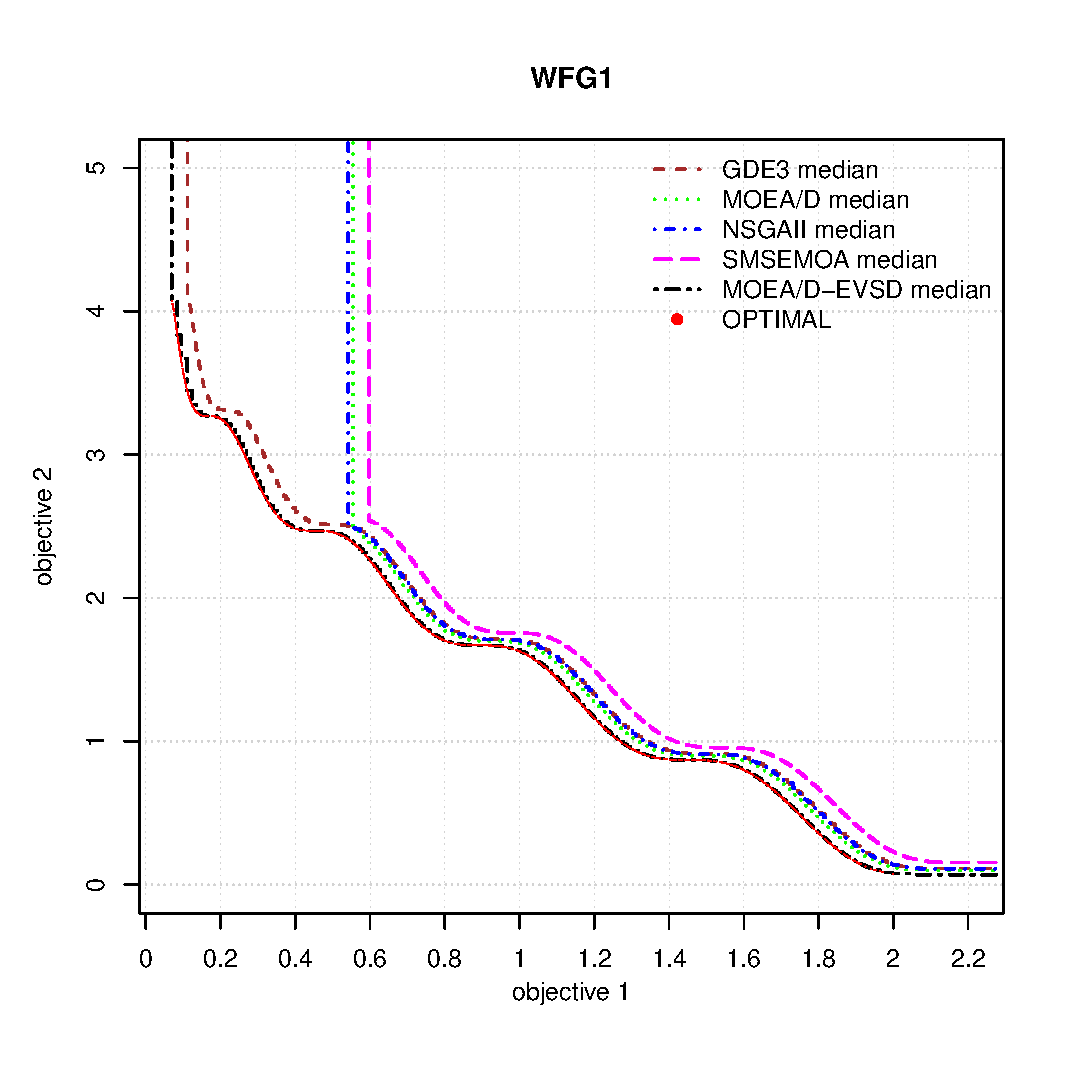
\includegraphics[width=0.33\textwidth]{Figures_Chapter7/Results_Chapter4/Surface_eps/WFG1.eps}  &
  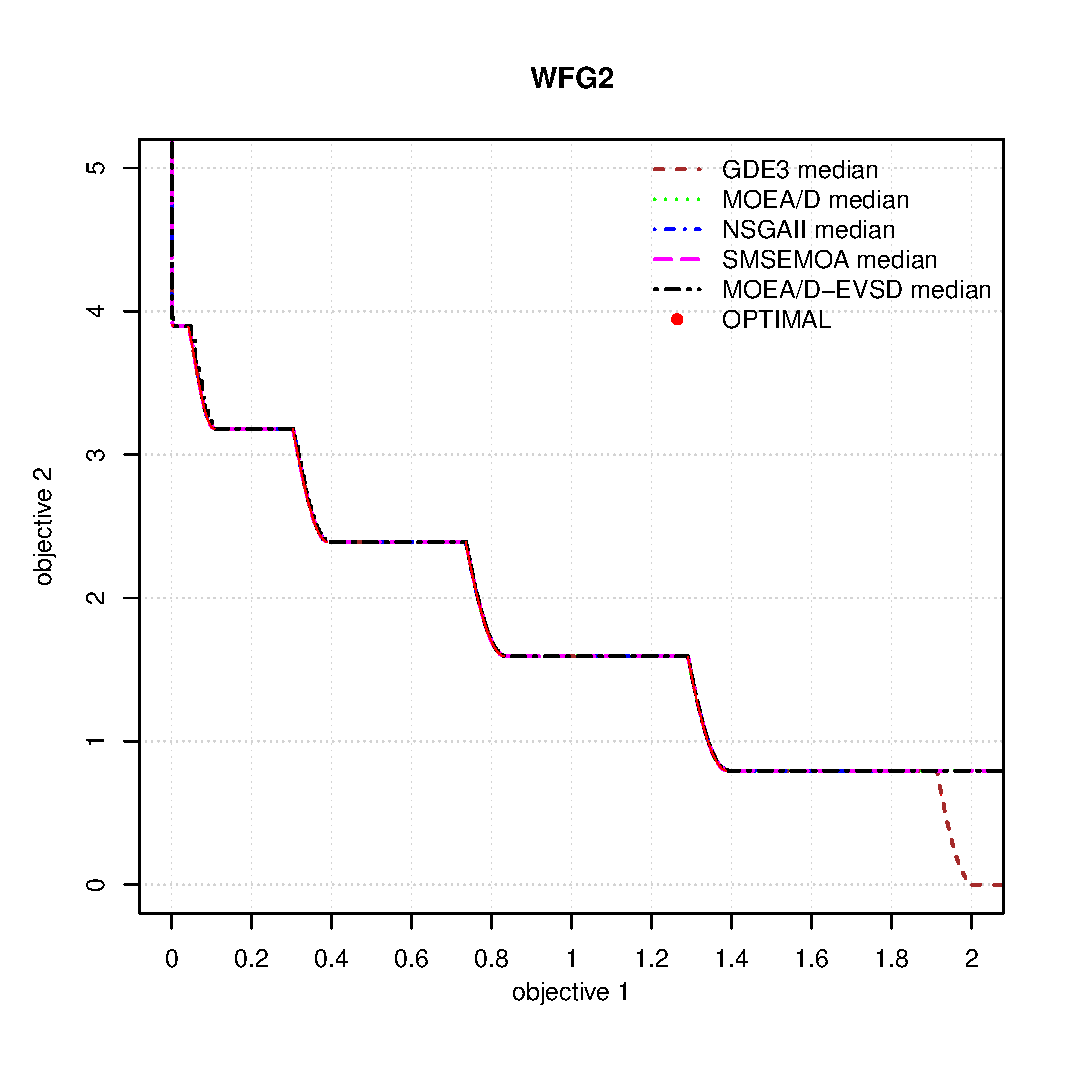
\includegraphics[width=0.33\textwidth]{Figures_Chapter7/Results_Chapter4/Surface_eps/WFG2.eps} &
  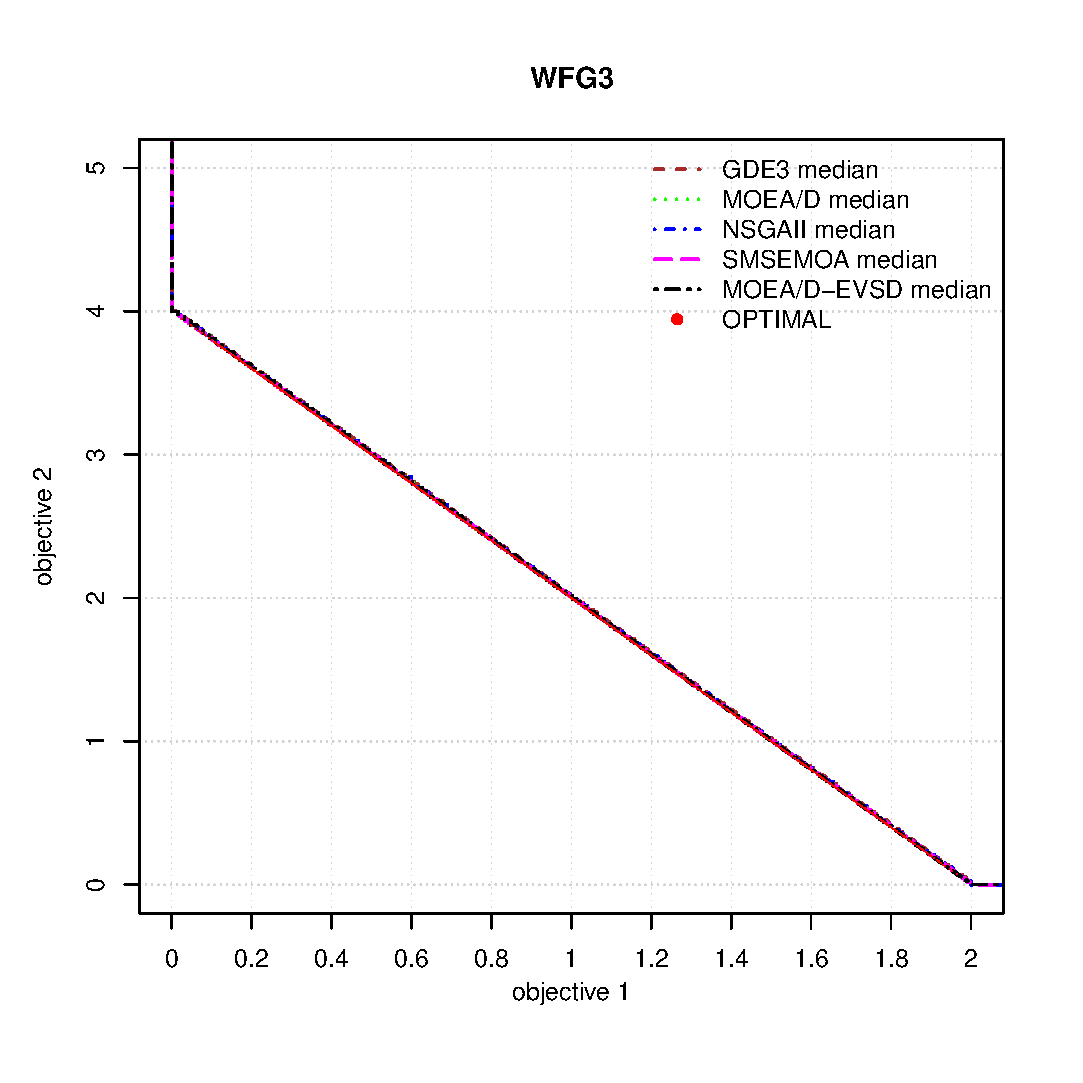
\includegraphics[width=0.33\textwidth]{Figures_Chapter7/Results_Chapter4/Surface_eps/WFG3.eps} \\
  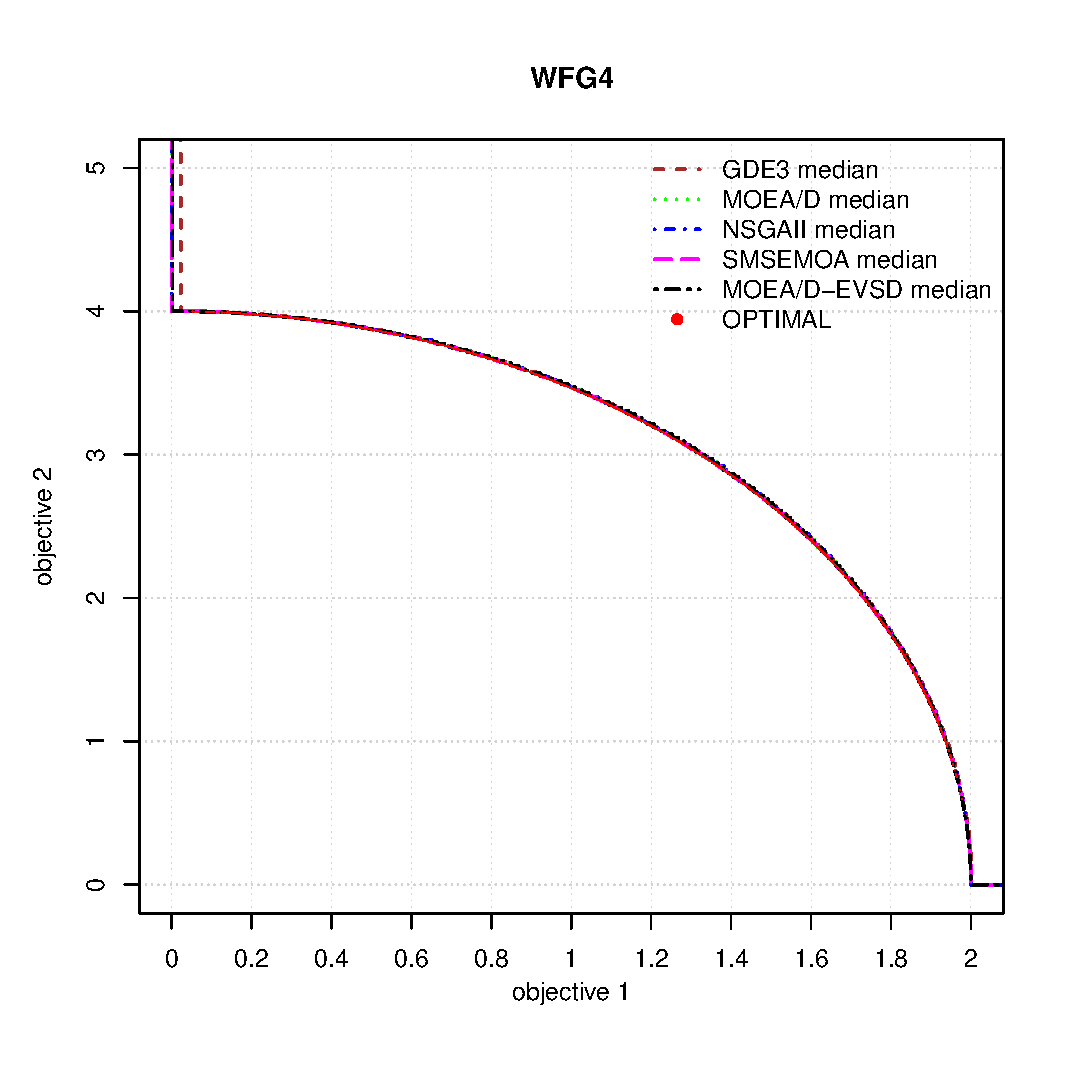
\includegraphics[width=0.33\textwidth]{Figures_Chapter7/Results_Chapter4/Surface_eps/WFG4.eps} &
  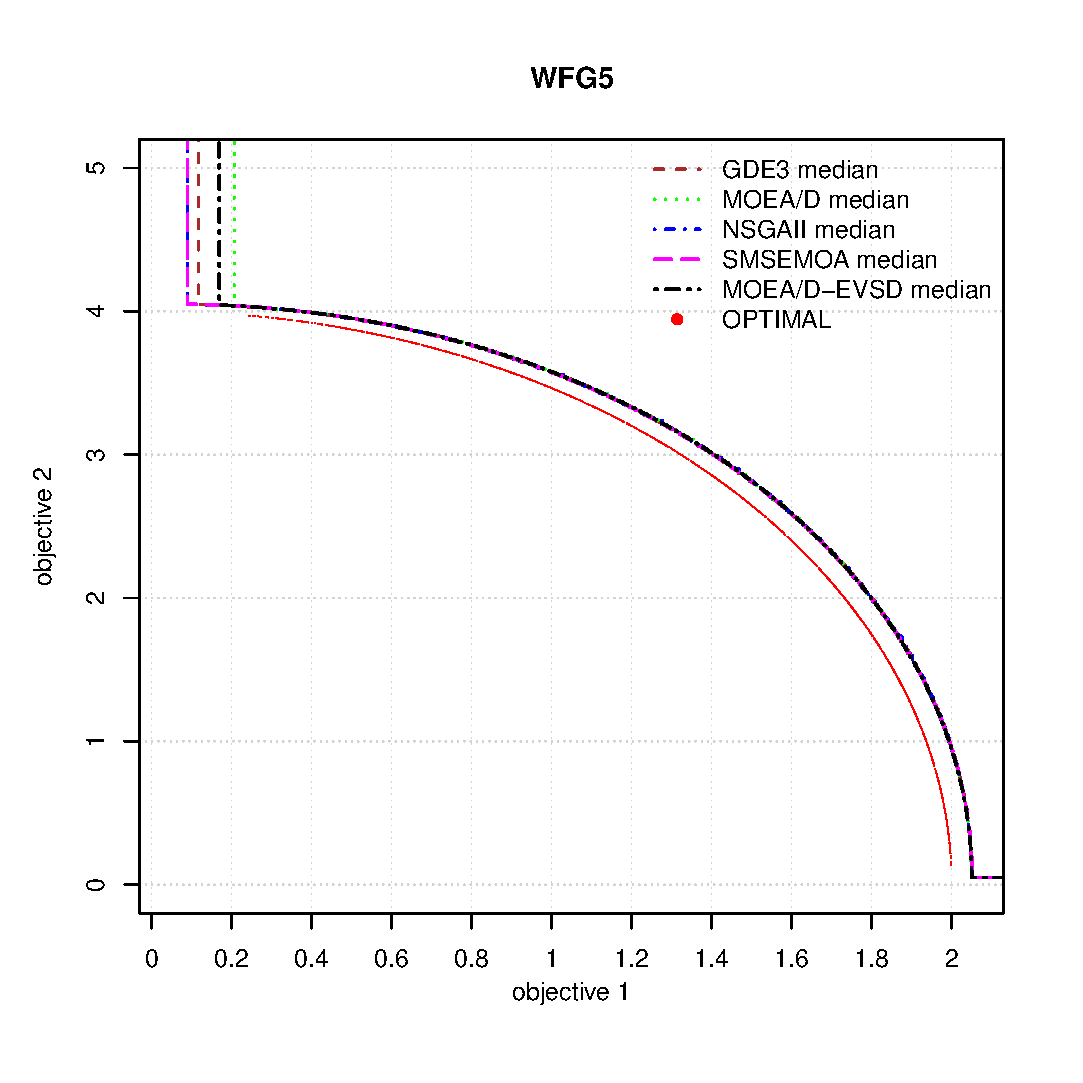
\includegraphics[width=0.33\textwidth]{Figures_Chapter7/Results_Chapter4/Surface_eps/WFG5.eps} &
  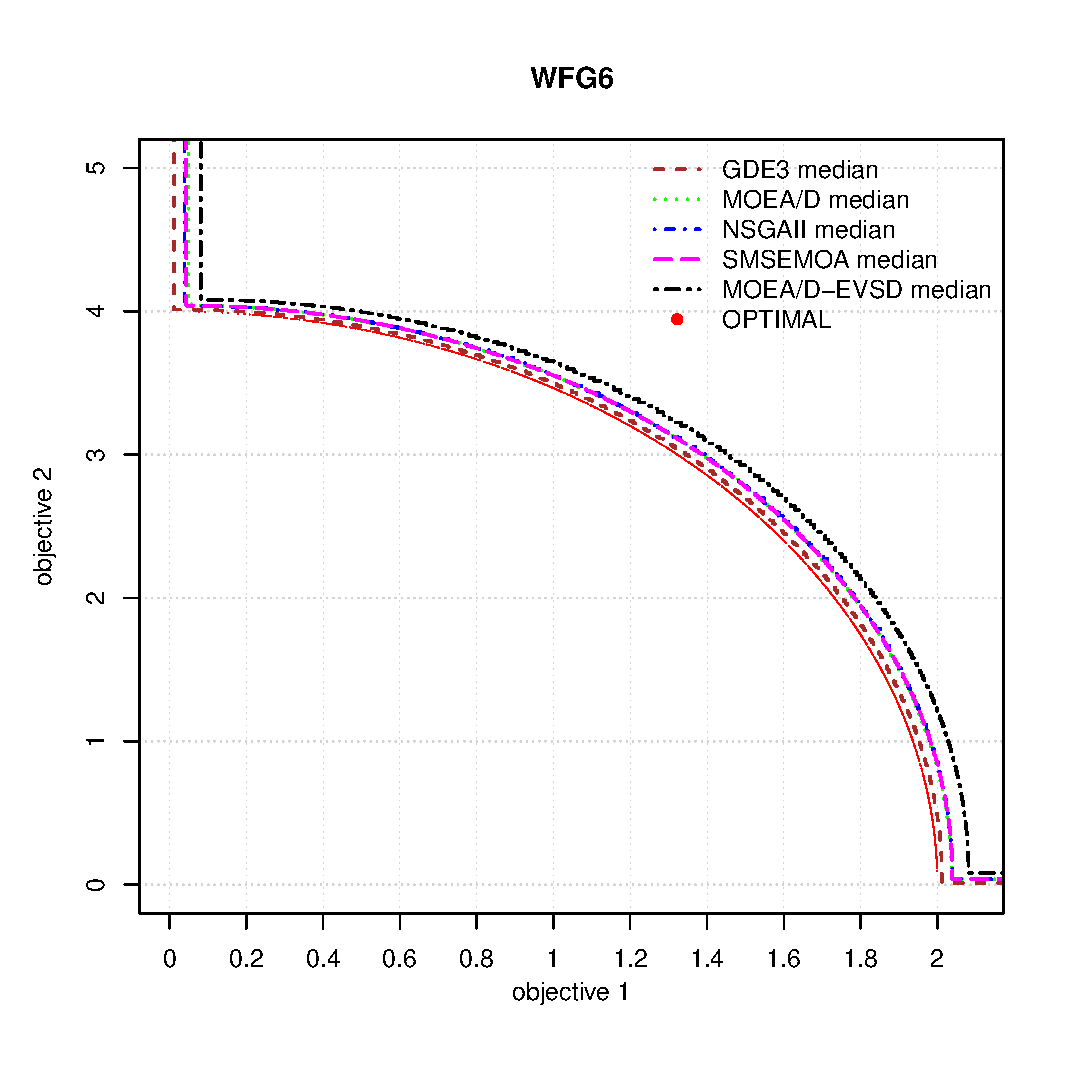
\includegraphics[width=0.33\textwidth]{Figures_Chapter7/Results_Chapter4/Surface_eps/WFG6.eps} \\
  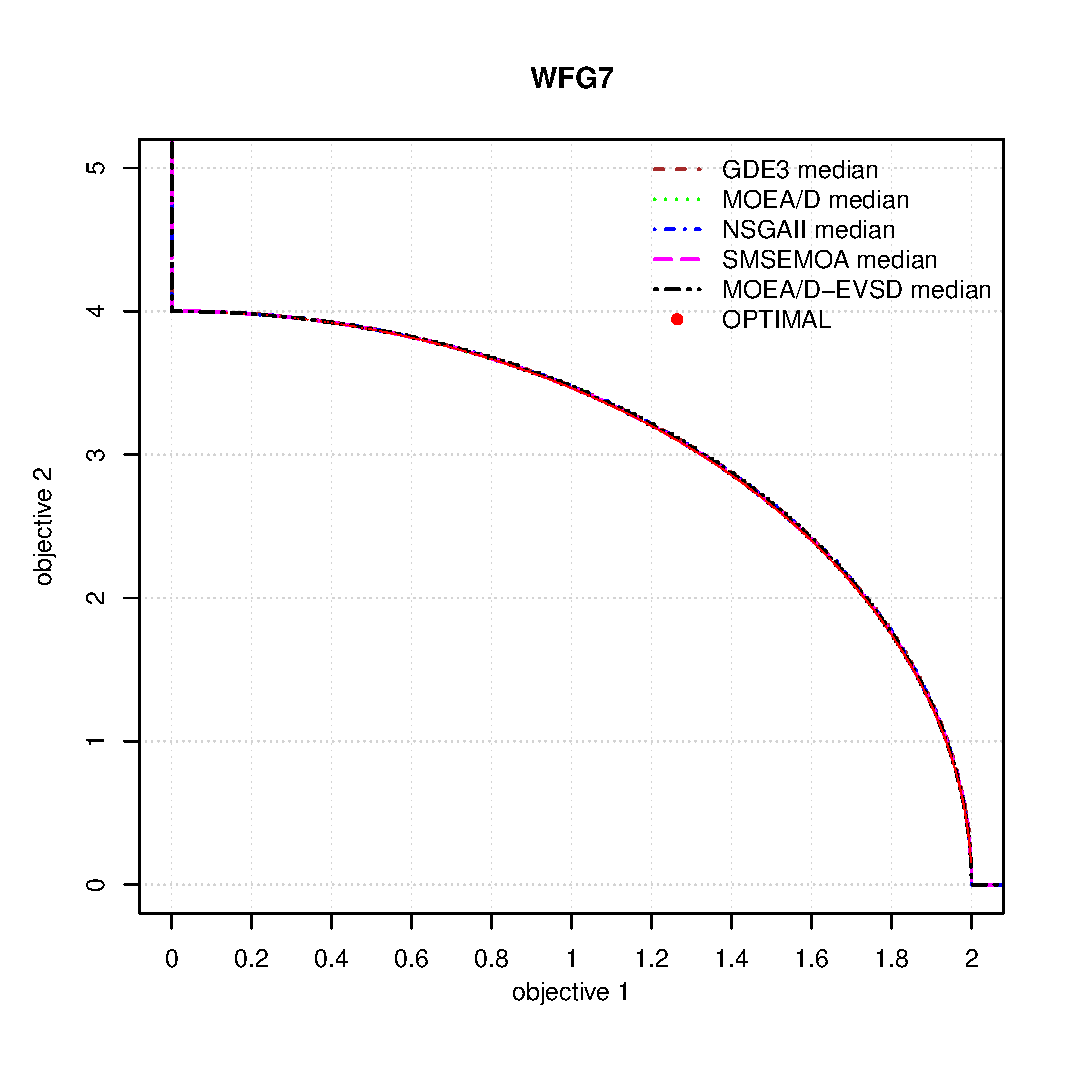
\includegraphics[width=0.33\textwidth]{Figures_Chapter7/Results_Chapter4/Surface_eps/WFG7.eps} &
  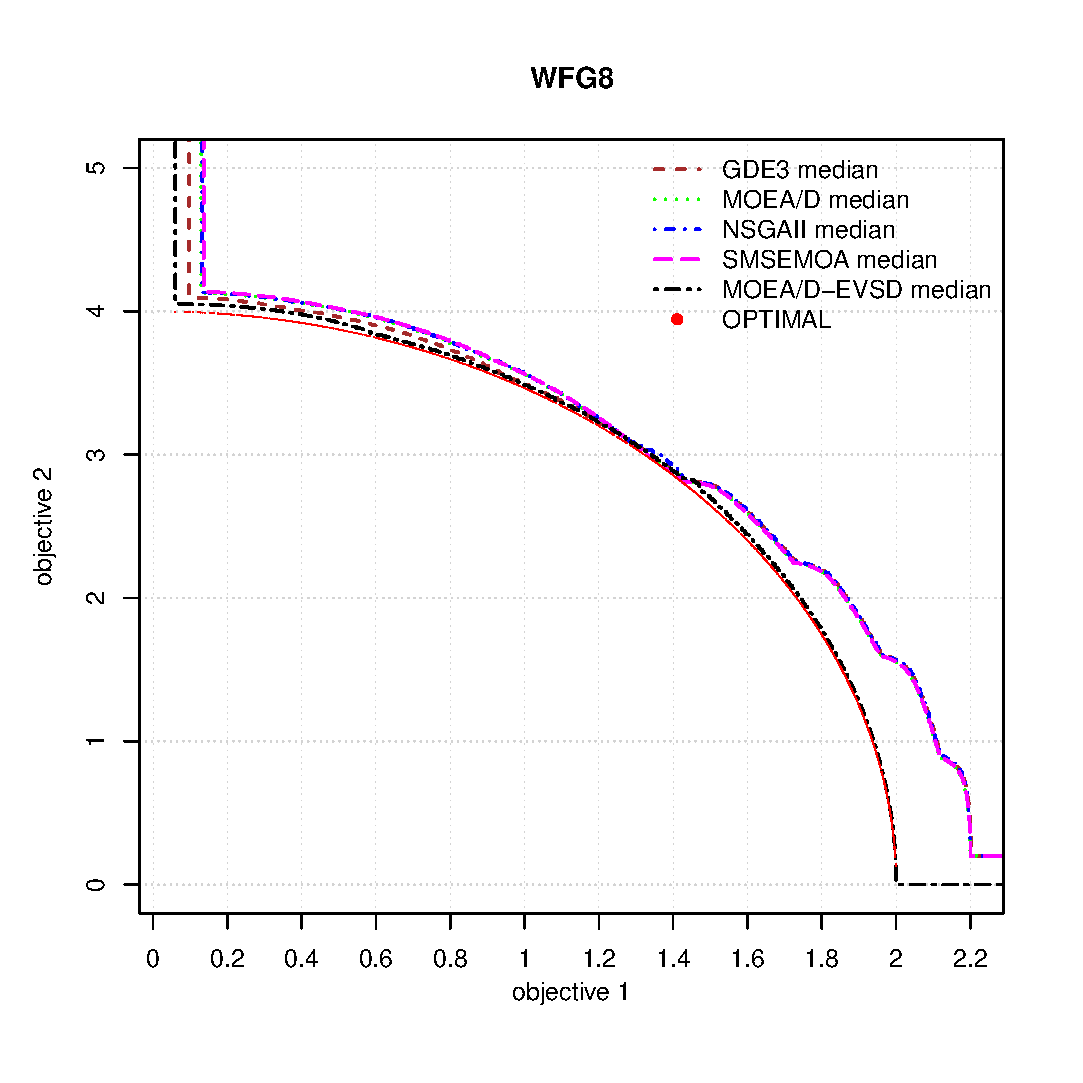
\includegraphics[width=0.33\textwidth]{Figures_Chapter7/Results_Chapter4/Surface_eps/WFG8.eps} &
  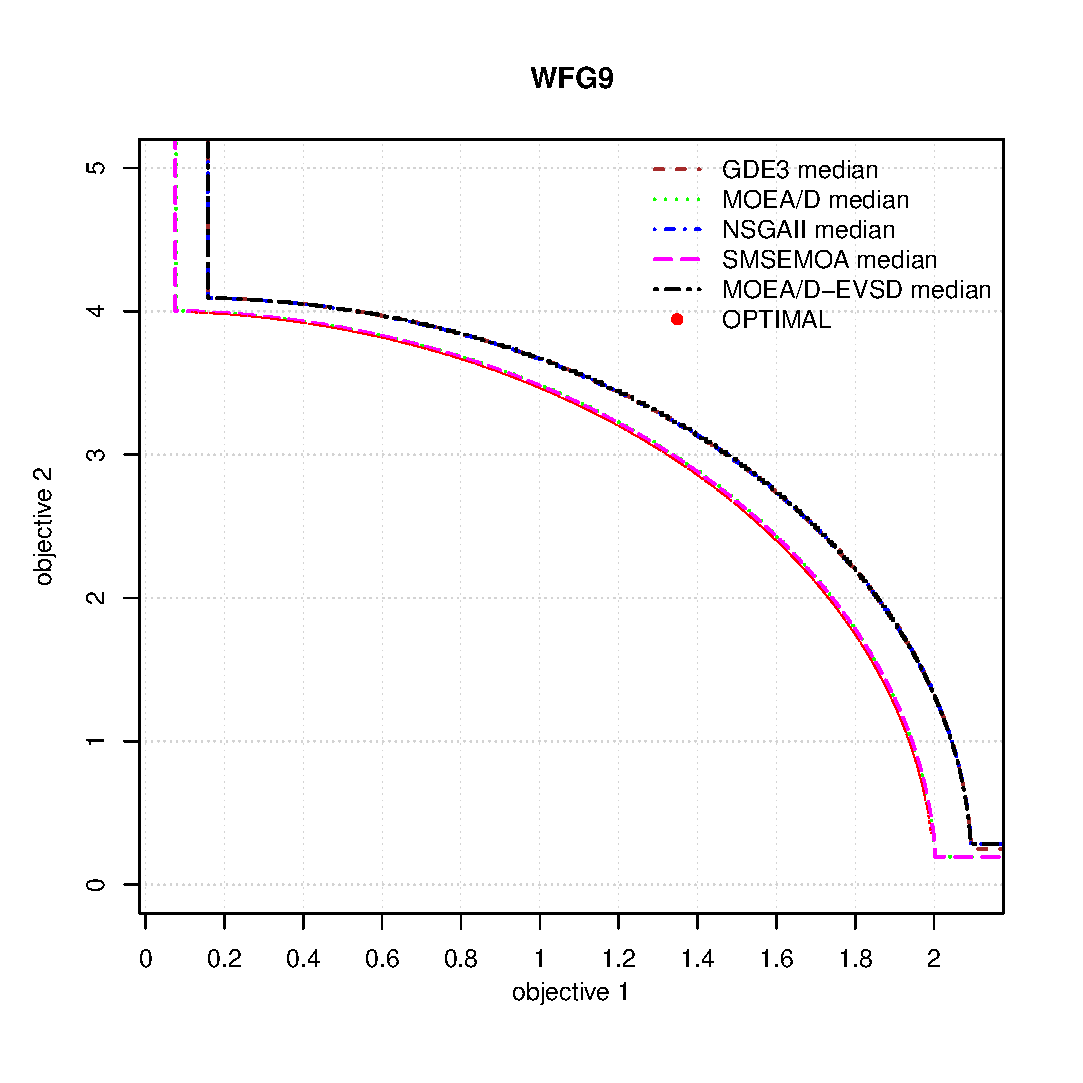
\includegraphics[width=0.33\textwidth]{Figures_Chapter7/Results_Chapter4/Surface_eps/WFG9.eps}
\end{tabular}
\end{figure}



% Please add the following required packages to your document preamble:
% \usepackage{graphicx}
\begin{table}[]
\centering
\caption{Estadísticas del hipervolumen considerando dos objetivos}
\label{my-label}
\resizebox{\textwidth}{!}{%
\begin{tabular}{c|c|c|c|c|c|c|c|c|c|c|c|c|c|c|c|}
\cline{2-16}
 & \multicolumn{3}{c|}{MOEA/D-SEBV} & \multicolumn{3}{c|}{VSD-MOEA/D T=10} & \multicolumn{3}{c|}{VSD-MOEA/D T=100} & \multicolumn{3}{c|}{VSD-MOEA/D Normal DE} & \multicolumn{3}{c|}{Fast VSD-MOEA/D} \\ \cline{2-16} 
 & Min & Max & Mean & Min & Max & Mean & Min & Max & Mean & Min & Max & Mean & Min & Max & Mean \\ \hline
\multicolumn{1}{|c|}{DTLZ1} & 1.081 & 1.081 & 1.081 & 1.081 & 1.081 & 1.081 & 1.081 & 1.081 & 1.081 & 1.084 & 1.084 & \textbf{1.084} & 1.081 & 1.081 & 1.081 \\ \hline
\multicolumn{1}{|c|}{DTLZ2} & 0.419 & 0.419 & 0.419 & 0.420 & 0.420 & \textbf{0.420} & 0.420 & 0.420 & \textbf{0.420} & 0.420 & 0.420 & \textbf{0.420} & 0.420 & 0.420 & \textbf{0.420} \\ \hline
\multicolumn{1}{|c|}{DTLZ3} & 8.190 & 8.190 & 8.190 & 8.210 & 8.210 & \textbf{8.210} & 8.210 & 8.210 & \textbf{8.210} & 8.210 & 8.210 & \textbf{8.210} & 8.210 & 8.210 & \textbf{8.210} \\ \hline
\multicolumn{1}{|c|}{DTLZ4} & 0.110 & 0.419 & 0.393 & 0.420 & 0.420 & \textbf{0.420} & 0.420 & 0.420 & \textbf{0.420} & 0.420 & 0.420 & \textbf{0.420} & 0.420 & 0.420 & \textbf{0.420} \\ \hline
\multicolumn{1}{|c|}{DTLZ5} & 8.190 & 8.190 & 8.190 & 8.210 & 8.210 & \textbf{8.210} & 8.210 & 8.210 & \textbf{8.210} & 8.210 & 8.210 & \textbf{8.210} & 8.210 & 8.210 & \textbf{8.210} \\ \hline
\multicolumn{1}{|c|}{DTLZ6} & 8.190 & 8.190 & 8.190 & 8.210 & 8.210 & \textbf{8.210} & 8.210 & 8.210 & \textbf{8.210} & 8.210 & 8.210 & \textbf{8.210} & 8.210 & 8.210 & \textbf{8.210} \\ \hline
\multicolumn{1}{|c|}{DTLZ7} & 0.891 & 0.891 & 0.891 & 0.892 & 0.892 & 0.892 & 0.892 & 0.892 & 0.892 & 0.893 & 0.893 & \textbf{0.893} & 0.892 & 0.892 & 0.892 \\ \hline
\multicolumn{1}{|c|}{UF1} & 3.648 & 3.650 & 3.649 & 3.650 & 3.652 & 3.651 & 3.650 & 3.651 & 3.651 & 3.655 & 3.660 & \textbf{3.658} & 3.650 & 3.652 & 3.651 \\ \hline
\multicolumn{1}{|c|}{UF2} & 3.633 & 3.647 & 3.642 & 3.648 & 3.651 & 3.649 & 3.647 & 3.652 & 3.650 & 3.656 & 3.660 & \textbf{3.659} & 3.647 & 3.651 & 3.649 \\ \hline
\multicolumn{1}{|c|}{UF3} & 3.498 & 3.651 & 3.632 & 3.652 & 3.654 & 3.653 & 3.646 & 3.655 & 3.652 & 3.660 & 3.661 & \textbf{3.660} & 3.650 & 3.655 & 3.652 \\ \hline
\multicolumn{1}{|c|}{UF4} & 3.158 & 3.215 & 3.189 & 3.246 & 3.263 & \textbf{3.253} & 3.240 & 3.261 & 3.249 & 3.230 & 3.244 & 3.236 & 3.240 & 3.264 & 3.250 \\ \hline
\multicolumn{1}{|c|}{UF5} & 3.404 & 3.459 & 3.411 & 3.470 & 3.475 & \textbf{3.475} & 3.474 & 3.475 & \textbf{3.475} & 3.234 & 3.459 & 3.413 & 3.475 & 3.475 & \textbf{3.475} \\ \hline
\multicolumn{1}{|c|}{UF6} & 3.266 & 3.423 & 3.414 & 3.429 & 3.431 & 3.430 & 3.430 & 3.431 & 3.430 & 3.434 & 3.434 & \textbf{3.434} & 3.429 & 3.430 & 3.430 \\ \hline
\multicolumn{1}{|c|}{UF7} & 3.483 & 3.484 & 3.484 & 3.483 & 3.484 & 3.483 & 3.483 & 3.484 & 3.484 & 3.494 & 3.494 & \textbf{3.494} & 3.483 & 3.485 & 3.484 \\ \hline
\multicolumn{1}{|c|}{WFG1} & 4.688 & 5.244 & 5.145 & 5.051 & 5.249 & \textbf{5.220} & 4.991 & 5.247 & 5.198 & 4.755 & 5.248 & 5.143 & 5.053 & 5.247 & 5.207 \\ \hline
\multicolumn{1}{|c|}{WFG2} & 5.056 & 5.056 & 5.056 & 5.057 & 5.057 & 5.057 & 5.057 & 5.057 & 5.057 & 5.059 & 5.059 & \textbf{5.059} & 5.057 & 5.057 & 5.057 \\ \hline
\multicolumn{1}{|c|}{WFG3} & 4.561 & 4.561 & 4.561 & 4.560 & 4.561 & 4.561 & 4.561 & 4.561 & 4.561 & 4.562 & 4.563 & \textbf{4.563} & 4.561 & 4.561 & 4.561 \\ \hline
\multicolumn{1}{|c|}{WFG4} & 2.283 & 2.284 & 2.284 & 2.282 & 2.283 & 2.283 & 2.282 & 2.283 & 2.283 & 2.283 & 2.286 & \textbf{2.285} & 2.282 & 2.283 & 2.283 \\ \hline
\multicolumn{1}{|c|}{WFG5} & 1.971 & 1.987 & 1.974 & 1.970 & 2.002 & 1.983 & 1.971 & 2.003 & 1.987 & 1.971 & 1.988 & 1.974 & 1.970 & 2.017 & \textbf{1.988} \\ \hline
\multicolumn{1}{|c|}{WFG6} & 1.705 & 2.284 & 1.953 & 2.255 & 2.284 & 2.282 & 2.283 & 2.284 & 2.283 & 2.150 & 2.285 & 2.271 & 2.283 & 2.286 & \textbf{2.284} \\ \hline
\multicolumn{1}{|c|}{WFG7} & 2.284 & 2.284 & \textbf{2.284} & 2.283 & 2.284 & \textbf{2.284} & 2.284 & 2.284 & \textbf{2.284} & 2.286 & 2.286 & 2.286 & 2.284 & 2.284 & \textbf{2.284} \\ \hline
\multicolumn{1}{|c|}{WFG8} & 1.862 & 1.878 & 1.870 & 2.107 & 2.265 & 2.237 & 2.248 & 2.275 & \textbf{2.260} & 2.226 & 2.264 & 2.237 & 2.243 & 2.270 & 2.259 \\ \hline
\multicolumn{1}{|c|}{WFG9} & 1.706 & 2.253 & 2.011 & 2.249 & 2.264 & 2.254 & 2.248 & 2.269 & \textbf{2.258} & 2.249 & 2.266 & 2.254 & 2.248 & 2.265 & 2.257 \\ \hline
\end{tabular}%
}
\end{table}


% Please add the following required packages to your document preamble:
% \usepackage{graphicx}
\begin{table}[]
\centering
\caption{Estadísticas de Hausdorff considerando dos objetivos}
\label{my-label}
\resizebox{\textwidth}{!}{%
\begin{tabular}{c|c|c|c|c|c|c|c|c|c|c|c|c|c|c|c|}
\cline{2-16}
 & \multicolumn{3}{c|}{MOEA/D-SEBV} & \multicolumn{3}{c|}{VSD-MOEA/D T=10} & \multicolumn{3}{c|}{VSD-MOEA/D T=100} & \multicolumn{3}{c|}{VSD-MOEA/D Normal DE} & \multicolumn{3}{c|}{Fast VSD-MOEA/D} \\ \cline{2-16} 
 & Min & Max & Mean & Min & Max & Mean & Min & Max & Mean & Min & Max & Mean & Min & Max & Mean \\ \hline
\multicolumn{1}{|c|}{DTLZ1} & 0.002 & 0.002 & \textbf{0.002} & 0.002 & 0.002 & \textbf{0.002} & 0.002 & 0.002 & \textbf{0.002} & 0.002 & 0.002 & \textbf{0.002} & 0.002 & 0.002 & \textbf{0.002} \\ \hline
\multicolumn{1}{|c|}{DTLZ2} & 0.004 & 0.004 & \textbf{0.004} & 0.004 & 0.004 & \textbf{0.004} & 0.004 & 0.004 & \textbf{0.004} & 0.004 & 0.004 & \textbf{0.004} & 0.004 & 0.004 & \textbf{0.004} \\ \hline
\multicolumn{1}{|c|}{DTLZ3} & 0.004 & 0.004 & \textbf{0.004} & 0.004 & 0.004 & \textbf{0.004} & 0.004 & 0.004 & \textbf{0.004} & 0.004 & 0.004 & \textbf{0.004} & 0.004 & 0.004 & \textbf{0.004} \\ \hline
\multicolumn{1}{|c|}{DTLZ4} & 0.004 & 0.746 & 0.068 & 0.004 & 0.004 & \textbf{0.004} & 0.004 & 0.004 & \textbf{0.004} & 0.004 & 0.004 & \textbf{0.004} & 0.004 & 0.004 & \textbf{0.004} \\ \hline
\multicolumn{1}{|c|}{DTLZ5} & 0.004 & 0.004 & \textbf{0.004} & 0.004 & 0.004 & \textbf{0.004} & 0.004 & 0.004 & \textbf{0.004} & 0.004 & 0.004 & \textbf{0.004} & 0.004 & 0.004 & \textbf{0.004} \\ \hline
\multicolumn{1}{|c|}{DTLZ6} & 0.004 & 0.004 & \textbf{0.004} & 0.004 & 0.004 & \textbf{0.004} & 0.004 & 0.004 & \textbf{0.004} & 0.004 & 0.004 & \textbf{0.004} & 0.004 & 0.004 & \textbf{0.004} \\ \hline
\multicolumn{1}{|c|}{DTLZ7} & 0.007 & 0.007 & \textbf{0.007} & 0.007 & 0.007 & \textbf{0.007} & 0.007 & 0.007 & \textbf{0.007} & 0.007 & 0.007 & \textbf{0.007} & 0.007 & 0.007 & \textbf{0.007} \\ \hline
\multicolumn{1}{|c|}{UF1} & 0.004 & 0.004 & \textbf{0.004} & 0.004 & 0.004 & \textbf{0.004} & 0.004 & 0.004 & \textbf{0.004} & 0.004 & 0.011 & 0.005 & 0.004 & 0.004 & \textbf{0.004} \\ \hline
\multicolumn{1}{|c|}{UF2} & 0.005 & 0.005 & 0.005 & 0.004 & 0.004 & \textbf{0.004} & 0.004 & 0.004 & \textbf{0.004} & 0.005 & 0.008 & 0.005 & 0.004 & 0.004 & \textbf{0.004} \\ \hline
\multicolumn{1}{|c|}{UF3} & 0.004 & 0.041 & 0.009 & 0.004 & 0.004 & \textbf{0.004} & 0.004 & 0.008 & \textbf{0.004} & 0.004 & 0.004 & \textbf{0.004} & 0.004 & 0.004 & \textbf{0.004} \\ \hline
\multicolumn{1}{|c|}{UF4} & 0.043 & 0.052 & 0.047 & 0.024 & 0.026 & \textbf{0.025} & 0.025 & 0.027 & 0.026 & 0.034 & 0.037 & 0.035 & 0.025 & 0.027 & 0.026 \\ \hline
\multicolumn{1}{|c|}{UF5} & 0.022 & 0.052 & 0.041 & 0.000 & 0.007 & \textbf{0.000} & 0.000 & 0.001 & \textbf{0.000} & 0.024 & 0.084 & 0.045 & 0.000 & 0.000 & \textbf{0.000} \\ \hline
\multicolumn{1}{|c|}{UF6} & 0.008 & 0.043 & 0.022 & 0.002 & 0.002 & \textbf{0.002} & 0.002 & 0.002 & \textbf{0.002} & 0.012 & 0.035 & 0.021 & 0.002 & 0.002 & \textbf{0.002} \\ \hline
\multicolumn{1}{|c|}{UF7} & 0.004 & 0.004 & \textbf{0.004} & 0.004 & 0.004 & \textbf{0.004} & 0.004 & 0.004 & \textbf{0.004} & 0.004 & 0.004 & \textbf{0.004} & 0.004 & 0.004 & \textbf{0.004} \\ \hline
\multicolumn{1}{|c|}{WFG1} & 0.025 & 0.131 & 0.045 & 0.035 & 0.105 & 0.065 & 0.041 & 0.206 & 0.058 & 0.021 & 0.122 & \textbf{0.039} & 0.044 & 0.205 & 0.060 \\ \hline
\multicolumn{1}{|c|}{WFG2} & 0.036 & 0.036 & 0.036 & 0.038 & 0.038 & 0.038 & 0.038 & 0.038 & 0.038 & 0.034 & 0.034 & \textbf{0.034} & 0.038 & 0.038 & 0.038 \\ \hline
\multicolumn{1}{|c|}{WFG3} & 0.013 & 0.013 & \textbf{0.013} & 0.013 & 0.013 & \textbf{0.013} & 0.013 & 0.013 & \textbf{0.013} & 0.013 & 0.013 & \textbf{0.013} & 0.013 & 0.013 & \textbf{0.013} \\ \hline
\multicolumn{1}{|c|}{WFG4} & 0.014 & 0.014 & \textbf{0.014} & 0.015 & 0.015 & 0.015 & 0.015 & 0.015 & 0.015 & 0.014 & 0.014 & \textbf{0.014} & 0.015 & 0.015 & 0.015 \\ \hline
\multicolumn{1}{|c|}{WFG5} & 0.064 & 0.069 & 0.068 & 0.062 & 0.070 & 0.066 & 0.061 & 0.069 & \textbf{0.065} & 0.064 & 0.069 & 0.068 & 0.059 & 0.070 & \textbf{0.065} \\ \hline
\multicolumn{1}{|c|}{WFG6} & 0.014 & 0.121 & 0.075 & 0.015 & 0.016 & \textbf{0.015} & 0.015 & 0.015 & \textbf{0.015} & 0.014 & 0.032 & \textbf{0.015} & 0.015 & 0.015 & \textbf{0.015} \\ \hline
\multicolumn{1}{|c|}{WFG7} & 0.014 & 0.014 & \textbf{0.014} & 0.015 & 0.015 & 0.015 & 0.015 & 0.015 & 0.015 & 0.014 & 0.014 & \textbf{0.014} & 0.015 & 0.015 & 0.015 \\ \hline
\multicolumn{1}{|c|}{WFG8} & 0.114 & 0.118 & 0.116 & 0.018 & 0.079 & 0.027 & 0.017 & 0.025 & \textbf{0.020} & 0.018 & 0.032 & 0.027 & 0.017 & 0.023 & \textbf{0.020} \\ \hline
\multicolumn{1}{|c|}{WFG9} & 0.015 & 0.126 & 0.064 & 0.015 & 0.017 & \textbf{0.016} & 0.015 & 0.017 & \textbf{0.016} & 0.014 & 0.017 & \textbf{0.016} & 0.015 & 0.017 & \textbf{0.016} \\ \hline
\end{tabular}%
}
\end{table}

% Please add the following required packages to your document preamble:
% \usepackage{graphicx}
\begin{table}[]
\centering
\caption{Estadísticas IGD+ considerando dos objetivos}
\label{my-label}
\resizebox{\textwidth}{!}{%
\begin{tabular}{c|c|c|c|c|c|c|c|c|c|c|c|c|c|c|c|}
\cline{2-16}
 & \multicolumn{3}{c|}{MOEA/D-SEBV} & \multicolumn{3}{c|}{VSD-MOEA/D T=10} & \multicolumn{3}{c|}{VSD-MOEA/D T=100} & \multicolumn{3}{c|}{VSD-MOEA/D Normal DE} & \multicolumn{3}{c|}{Fast VSD-MOEA/D} \\ \cline{2-16} 
 & Min & Max & Mean & Min & Max & Mean & Min & Max & Mean & Min & Max & Mean & Min & Max & Mean \\ \hline
\multicolumn{1}{|c|}{DTLZ1} & 0.001 & 0.001 & \textbf{0.001} & 0.001 & 0.001 & \textbf{0.001} & 0.001 & 0.001 & \textbf{0.001} & 0.001 & 0.001 & \textbf{0.001} & 0.001 & 0.001 & \textbf{0.001} \\ \hline
\multicolumn{1}{|c|}{DTLZ2} & 0.002 & 0.002 & \textbf{0.002} & 0.002 & 0.002 & \textbf{0.002} & 0.002 & 0.002 & \textbf{0.002} & 0.002 & 0.002 & \textbf{0.002} & 0.002 & 0.002 & \textbf{0.002} \\ \hline
\multicolumn{1}{|c|}{DTLZ3} & 0.002 & 0.002 & \textbf{0.002} & 0.002 & 0.002 & \textbf{0.002} & 0.002 & 0.002 & \textbf{0.002} & 0.002 & 0.002 & \textbf{0.002} & 0.002 & 0.002 & \textbf{0.002} \\ \hline
\multicolumn{1}{|c|}{DTLZ4} & 0.002 & 0.363 & 0.033 & 0.002 & 0.002 & \textbf{0.002} & 0.002 & 0.002 & \textbf{0.002} & 0.002 & 0.002 & \textbf{0.002} & 0.002 & 0.002 & \textbf{0.002} \\ \hline
\multicolumn{1}{|c|}{DTLZ5} & 0.002 & 0.002 & \textbf{0.002} & 0.002 & 0.002 & \textbf{0.002} & 0.002 & 0.002 & \textbf{0.002} & 0.002 & 0.002 & \textbf{0.002} & 0.002 & 0.002 & \textbf{0.002} \\ \hline
\multicolumn{1}{|c|}{DTLZ6} & 0.002 & 0.002 & \textbf{0.002} & 0.002 & 0.002 & \textbf{0.002} & 0.002 & 0.002 & \textbf{0.002} & 0.002 & 0.002 & \textbf{0.002} & 0.002 & 0.002 & \textbf{0.002} \\ \hline
\multicolumn{1}{|c|}{DTLZ7} & 0.003 & 0.003 & \textbf{0.003} & 0.003 & 0.003 & \textbf{0.003} & 0.003 & 0.003 & \textbf{0.003} & 0.003 & 0.003 & \textbf{0.003} & 0.003 & 0.003 & \textbf{0.003} \\ \hline
\multicolumn{1}{|c|}{UF1} & 0.003 & 0.003 & \textbf{0.003} & 0.003 & 0.003 & \textbf{0.003} & 0.002 & 0.003 & \textbf{0.003} & 0.003 & 0.003 & \textbf{0.003} & 0.002 & 0.003 & \textbf{0.003} \\ \hline
\multicolumn{1}{|c|}{UF2} & 0.004 & 0.004 & 0.004 & 0.003 & 0.003 & \textbf{0.003} & 0.003 & 0.003 & \textbf{0.003} & 0.004 & 0.004 & 0.004 & 0.003 & 0.003 & \textbf{0.003} \\ \hline
\multicolumn{1}{|c|}{UF3} & 0.003 & 0.036 & 0.007 & 0.002 & 0.002 & \textbf{0.002} & 0.003 & 0.007 & 0.003 & 0.003 & 0.003 & 0.003 & 0.003 & 0.003 & 0.003 \\ \hline
\multicolumn{1}{|c|}{UF4} & 0.042 & 0.050 & 0.045 & 0.023 & 0.026 & \textbf{0.024} & 0.024 & 0.026 & 0.025 & 0.033 & 0.037 & 0.035 & 0.023 & 0.026 & 0.025 \\ \hline
\multicolumn{1}{|c|}{UF5} & 0.006 & 0.040 & 0.036 & 0.000 & 0.005 & \textbf{0.000} & 0.000 & 0.000 & \textbf{0.000} & 0.015 & 0.040 & 0.030 & 0.000 & 0.000 & \textbf{0.000} \\ \hline
\multicolumn{1}{|c|}{UF6} & 0.002 & 0.018 & 0.003 & 0.002 & 0.002 & \textbf{0.002} & 0.002 & 0.002 & \textbf{0.002} & 0.002 & 0.002 & \textbf{0.002} & 0.002 & 0.002 & \textbf{0.002} \\ \hline
\multicolumn{1}{|c|}{UF7} & 0.003 & 0.003 & \textbf{0.003} & 0.003 & 0.003 & \textbf{0.003} & 0.003 & 0.003 & \textbf{0.003} & 0.003 & 0.003 & \textbf{0.003} & 0.003 & 0.003 & \textbf{0.003} \\ \hline
\multicolumn{1}{|c|}{WFG1} & 0.007 & 0.122 & 0.028 & 0.007 & 0.046 & \textbf{0.013} & 0.007 & 0.059 & 0.017 & 0.007 & 0.108 & 0.027 & 0.007 & 0.048 & 0.015 \\ \hline
\multicolumn{1}{|c|}{WFG2} & 0.006 & 0.006 & \textbf{0.006} & 0.006 & 0.006 & \textbf{0.006} & 0.006 & 0.006 & \textbf{0.006} & 0.006 & 0.006 & \textbf{0.006} & 0.006 & 0.006 & \textbf{0.006} \\ \hline
\multicolumn{1}{|c|}{WFG3} & 0.008 & 0.008 & \textbf{0.008} & 0.008 & 0.008 & \textbf{0.008} & 0.008 & 0.008 & \textbf{0.008} & 0.008 & 0.008 & \textbf{0.008} & 0.008 & 0.008 & \textbf{0.008} \\ \hline
\multicolumn{1}{|c|}{WFG4} & 0.007 & 0.007 & \textbf{0.007} & 0.007 & 0.007 & \textbf{0.007} & 0.007 & 0.007 & \textbf{0.007} & 0.007 & 0.007 & \textbf{0.007} & 0.007 & 0.007 & \textbf{0.007} \\ \hline
\multicolumn{1}{|c|}{WFG5} & 0.064 & 0.069 & 0.067 & 0.061 & 0.070 & 0.066 & 0.061 & 0.069 & \textbf{0.065} & 0.064 & 0.069 & 0.068 & 0.059 & 0.070 & \textbf{0.065} \\ \hline
\multicolumn{1}{|c|}{WFG6} & 0.007 & 0.121 & 0.072 & 0.007 & 0.012 & \textbf{0.007} & 0.007 & 0.007 & \textbf{0.007} & 0.007 & 0.031 & 0.009 & 0.007 & 0.007 & \textbf{0.007} \\ \hline
\multicolumn{1}{|c|}{WFG7} & 0.007 & 0.007 & \textbf{0.007} & 0.007 & 0.007 & \textbf{0.007} & 0.007 & 0.007 & \textbf{0.007} & 0.007 & 0.007 & \textbf{0.007} & 0.007 & 0.007 & \textbf{0.007} \\ \hline
\multicolumn{1}{|c|}{WFG8} & 0.092 & 0.097 & 0.094 & 0.011 & 0.039 & 0.018 & 0.009 & 0.016 & \textbf{0.012} & 0.011 & 0.021 & 0.018 & 0.009 & 0.017 & \textbf{0.012} \\ \hline
\multicolumn{1}{|c|}{WFG9} & 0.011 & 0.126 & 0.062 & 0.010 & 0.012 & 0.012 & 0.009 & 0.013 & \textbf{0.011} & 0.009 & 0.012 & \textbf{0.011} & 0.010 & 0.013 & \textbf{0.011} \\ \hline
\end{tabular}%
}
\end{table}


% Please add the following required packages to your document preamble:
% \usepackage{graphicx}
\begin{table}[]
\centering
\caption{Estadísticas del hipervolumen considerando tres objetivos}
\label{my-label}
\resizebox{\textwidth}{!}{%
\begin{tabular}{c|c|c|c|c|c|c|c|c|c|c|c|c|c|c|c|}
\cline{2-16}
 & \multicolumn{3}{c|}{MOEA/D-SEBV} & \multicolumn{3}{c|}{VSD-MOEA/D T=10} & \multicolumn{3}{c|}{VSD-MOEA/D T=100} & \multicolumn{3}{c|}{VSD-MOEA/D Normal DE} & \multicolumn{3}{c|}{Fast VSD-MOEA/D} \\ \cline{2-16} 
 & Min & Max & Mean & Min & Max & Mean & Min & Max & Mean & Min & Max & Mean & Min & Max & Mean \\ \hline
\multicolumn{1}{|c|}{DTLZ1} & 1.289 & 1.289 & 1.289 & 1.293 & 1.293 & 1.293 & 1.293 & 1.293 & 1.293 & 1.296 & 1.296 & \textbf{1.296} & 1.293 & 1.293 & 1.293 \\ \hline
\multicolumn{1}{|c|}{DTLZ2} & 0.709 & 0.710 & 0.710 & 0.733 & 0.734 & \textbf{0.734} & 0.733 & 0.734 & 0.733 & 0.720 & 0.720 & 0.720 & 0.733 & 0.734 & 0.733 \\ \hline
\multicolumn{1}{|c|}{DTLZ3} & 26.158 & 26.162 & 26.159 & 26.402 & 26.403 & \textbf{26.403} & 26.402 & 26.403 & 26.402 & 26.263 & 26.267 & 26.264 & 26.402 & 26.403 & 26.402 \\ \hline
\multicolumn{1}{|c|}{DTLZ4} & 0.709 & 0.710 & 0.709 & 0.733 & 0.736 & \textbf{0.735} & 0.733 & 0.735 & 0.734 & 0.720 & 0.720 & 0.720 & 0.733 & 0.734 & 0.734 \\ \hline
\multicolumn{1}{|c|}{DTLZ5} & 23.877 & 23.877 & 23.877 & 23.900 & 23.900 & 23.900 & 23.900 & 23.900 & 23.900 & 23.975 & 23.975 & \textbf{23.975} & 23.900 & 23.900 & 23.900 \\ \hline
\multicolumn{1}{|c|}{DTLZ6} & 23.877 & 23.877 & 23.877 & 23.900 & 23.900 & 23.900 & 23.900 & 23.900 & 23.900 & 23.975 & 23.975 & \textbf{23.975} & 23.900 & 23.900 & 23.900 \\ \hline
\multicolumn{1}{|c|}{DTLZ7} & 1.764 & 1.764 & 1.764 & 1.756 & 1.756 & 1.756 & 1.756 & 1.756 & 1.756 & 1.777 & 1.777 & \textbf{1.777} & 1.756 & 1.756 & 1.756 \\ \hline
\multicolumn{1}{|c|}{UF10} & 4.000 & 7.186 & 5.155 & 7.265 & 7.360 & 7.310 & 7.275 & 7.370 & \textbf{7.323} & 6.339 & 7.157 & 6.923 & 7.289 & 7.361 & 7.319 \\ \hline
\multicolumn{1}{|c|}{UF8} & 4.000 & 7.290 & 7.083 & 7.403 & 7.409 & 7.407 & 7.406 & 7.412 & \textbf{7.409} & 7.260 & 7.317 & 7.295 & 7.405 & 7.412 & \textbf{7.409} \\ \hline
\multicolumn{1}{|c|}{UF9} & 7.096 & 7.638 & 7.195 & 7.684 & 7.713 & \textbf{7.700} & 7.684 & 7.705 & 7.693 & 7.623 & 7.679 & 7.654 & 7.682 & 7.706 & 7.693 \\ \hline
\multicolumn{1}{|c|}{WFG1} & 16.179 & 18.450 & 16.765 & 44.815 & 45.396 & \textbf{45.253} & 41.031 & 43.456 & 42.356 & 18.579 & 27.879 & 22.992 & 41.336 & 43.595 & 42.329 \\ \hline
\multicolumn{1}{|c|}{WFG2} & 47.579 & 47.977 & 47.741 & 47.826 & 47.831 & \textbf{47.827} & 47.826 & 47.828 & \textbf{47.827} & 47.162 & 47.910 & 47.703 & 47.826 & 47.827 & \textbf{47.827} \\ \hline
\multicolumn{1}{|c|}{WFG3} & 31.146 & 31.154 & 31.150 & 31.205 & 31.206 & 31.205 & 31.205 & 31.206 & 31.205 & 31.298 & 31.304 & \textbf{31.303} & 31.205 & 31.206 & 31.205 \\ \hline
\multicolumn{1}{|c|}{WFG4} & 21.261 & 22.007 & 21.644 & 23.189 & 23.346 & \textbf{23.257} & 23.184 & 23.309 & 23.240 & 21.238 & 21.857 & 21.563 & 23.172 & 23.301 & 23.241 \\ \hline
\multicolumn{1}{|c|}{WFG5} & 19.649 & 19.789 & 19.687 & 20.615 & 21.076 & 20.756 & 20.646 & 21.101 & \textbf{20.916} & 19.724 & 20.031 & 19.896 & 20.609 & 21.088 & 20.901 \\ \hline
\multicolumn{1}{|c|}{WFG6} & 18.053 & 22.220 & 18.867 & 22.172 & 23.228 & 23.019 & 22.908 & 23.251 & 23.180 & 20.960 & 22.221 & 21.402 & 23.039 & 23.267 & \textbf{23.195} \\ \hline
\multicolumn{1}{|c|}{WFG7} & 21.914 & 22.271 & 22.127 & 23.180 & 23.284 & 23.220 & 23.163 & 23.292 & \textbf{23.228} & 21.960 & 22.294 & 22.087 & 23.186 & 23.286 & 23.222 \\ \hline
\multicolumn{1}{|c|}{WFG8} & 18.671 & 20.020 & 18.942 & 20.059 & 23.425 & 22.887 & 23.092 & 23.526 & \textbf{23.298} & 21.017 & 21.683 & 21.325 & 23.109 & 23.461 & 23.289 \\ \hline
\multicolumn{1}{|c|}{WFG9} & 17.544 & 21.437 & 18.181 & 21.921 & 22.632 & 22.314 & 22.260 & 22.676 & 22.433 & 21.242 & 21.690 & 21.408 & 22.255 & 22.672 & \textbf{22.436} \\ \hline
\end{tabular}%
}
\end{table}



% Please add the following required packages to your document preamble:
% \usepackage{graphicx}
\begin{table}[]
\centering
\caption{Estadísticas con Hausdorff considerando tres objetivos}
\label{my-label}
\resizebox{\textwidth}{!}{%
\begin{tabular}{c|c|c|c|c|c|c|c|c|c|c|c|c|c|c|c|}
\cline{2-16}
 & \multicolumn{3}{c|}{MOEA/D-SEBV} & \multicolumn{3}{c|}{VSD-MOEA/D T=10} & \multicolumn{3}{c|}{VSD-MOEA/D T=100} & \multicolumn{3}{c|}{VSD-MOEA/D Normal DE} & \multicolumn{3}{c|}{Fast VSD-MOEA/D} \\ \cline{2-16} 
 & Min & Max & Mean & Min & Max & Mean & Min & Max & Mean & Min & Max & Mean & Min & Max & Mean \\ \hline
\multicolumn{1}{|c|}{DTLZ1} & 0.021 & 0.021 & 0.021 & 0.019 & 0.019 & \textbf{0.019} & 0.019 & 0.019 & \textbf{0.019} & 0.021 & 0.021 & 0.021 & 0.019 & 0.019 & \textbf{0.019} \\ \hline
\multicolumn{1}{|c|}{DTLZ2} & 0.054 & 0.054 & 0.054 & 0.051 & 0.051 & \textbf{0.051} & 0.051 & 0.051 & \textbf{0.051} & 0.054 & 0.054 & 0.054 & 0.051 & 0.051 & \textbf{0.051} \\ \hline
\multicolumn{1}{|c|}{DTLZ3} & 0.054 & 0.054 & 0.054 & 0.051 & 0.051 & \textbf{0.051} & 0.051 & 0.051 & \textbf{0.051} & 0.054 & 0.054 & 0.054 & 0.051 & 0.051 & \textbf{0.051} \\ \hline
\multicolumn{1}{|c|}{DTLZ4} & 0.054 & 0.054 & 0.054 & 0.051 & 0.051 & \textbf{0.051} & 0.051 & 0.051 & \textbf{0.051} & 0.054 & 0.054 & 0.054 & 0.051 & 0.051 & \textbf{0.051} \\ \hline
\multicolumn{1}{|c|}{DTLZ5} & 0.007 & 0.007 & \textbf{0.007} & 0.007 & 0.007 & \textbf{0.007} & 0.007 & 0.007 & \textbf{0.007} & 0.007 & 0.007 & \textbf{0.007} & 0.007 & 0.007 & \textbf{0.007} \\ \hline
\multicolumn{1}{|c|}{DTLZ6} & 0.007 & 0.007 & \textbf{0.007} & 0.007 & 0.007 & \textbf{0.007} & 0.007 & 0.007 & \textbf{0.007} & 0.007 & 0.007 & \textbf{0.007} & 0.007 & 0.007 & \textbf{0.007} \\ \hline
\multicolumn{1}{|c|}{DTLZ7} & 0.110 & 0.110 & \textbf{0.110} & 0.109 & 0.110 & \textbf{0.110} & 0.109 & 0.110 & \textbf{0.110} & 0.115 & 0.115 & 0.115 & 0.110 & 0.110 & \textbf{0.110} \\ \hline
\multicolumn{1}{|c|}{UF10} & 0.094 & 1.127 & 0.494 & 0.161 & 0.273 & 0.245 & 0.138 & 0.273 & 0.220 & 0.094 & 0.584 & \textbf{0.219} & 0.148 & 0.272 & 0.225 \\ \hline
\multicolumn{1}{|c|}{UF8} & 0.060 & 0.745 & 0.106 & 0.052 & 0.054 & \textbf{0.053} & 0.053 & 0.056 & 0.054 & 0.058 & 0.060 & 0.059 & 0.053 & 0.056 & 0.054 \\ \hline
\multicolumn{1}{|c|}{UF9} & 0.044 & 0.175 & 0.148 & 0.035 & 0.036 & \textbf{0.035} & 0.036 & 0.037 & 0.036 & 0.044 & 0.097 & 0.053 & 0.036 & 0.037 & 0.036 \\ \hline
\multicolumn{1}{|c|}{WFG1} & 1.177 & 1.266 & 1.227 & 0.310 & 0.431 & 0.340 & 0.264 & 0.468 & \textbf{0.333} & 0.716 & 1.114 & 0.936 & 0.268 & 0.430 & 0.339 \\ \hline
\multicolumn{1}{|c|}{WFG2} & 0.442 & 0.462 & 0.452 & 0.447 & 0.448 & 0.447 & 0.447 & 0.448 & 0.447 & 0.231 & 0.458 & \textbf{0.422} & 0.447 & 0.448 & 0.447 \\ \hline
\multicolumn{1}{|c|}{WFG3} & 0.508 & 0.509 & 0.509 & 0.446 & 0.446 & \textbf{0.446} & 0.446 & 0.446 & \textbf{0.446} & 0.490 & 0.490 & 0.490 & 0.446 & 0.446 & \textbf{0.446} \\ \hline
\multicolumn{1}{|c|}{WFG4} & 0.244 & 0.251 & 0.247 & 0.237 & 0.243 & 0.238 & 0.237 & 0.243 & 0.238 & 0.251 & 0.260 & 0.254 & 0.237 & 0.238 & \textbf{0.237} \\ \hline
\multicolumn{1}{|c|}{WFG5} & 0.259 & 0.262 & 0.261 & 0.247 & 0.254 & \textbf{0.249} & 0.247 & 0.256 & 0.250 & 0.259 & 0.264 & 0.263 & 0.247 & 0.254 & 0.250 \\ \hline
\multicolumn{1}{|c|}{WFG6} & 0.244 & 0.295 & 0.285 & 0.237 & 0.245 & 0.240 & 0.236 & 0.243 & \textbf{0.238} & 0.246 & 0.252 & 0.249 & 0.237 & 0.243 & \textbf{0.238} \\ \hline
\multicolumn{1}{|c|}{WFG7} & 0.244 & 0.245 & 0.245 & 0.237 & 0.237 & \textbf{0.237} & 0.237 & 0.237 & \textbf{0.237} & 0.246 & 0.247 & 0.246 & 0.236 & 0.237 & \textbf{0.237} \\ \hline
\multicolumn{1}{|c|}{WFG8} & 0.277 & 0.294 & 0.285 & 0.239 & 0.264 & 0.247 & 0.239 & 0.251 & \textbf{0.244} & 0.262 & 0.279 & 0.270 & 0.241 & 0.248 & 0.245 \\ \hline
\multicolumn{1}{|c|}{WFG9} & 0.241 & 0.296 & 0.285 & 0.230 & 0.240 & \textbf{0.235} & 0.230 & 0.238 & \textbf{0.235} & 0.243 & 0.248 & 0.246 & 0.230 & 0.239 & \textbf{0.235} \\ \hline
\end{tabular}%
}
\end{table}

% Please add the following required packages to your document preamble:
% \usepackage{graphicx}
\begin{table}[]
\centering
\caption{Estadísticas del IGD considerando tres objetivos}
\label{my-label}
\resizebox{\textwidth}{!}{%
\begin{tabular}{c|c|c|c|c|c|c|c|c|c|c|c|c|c|c|c|}
\cline{2-16}
 & \multicolumn{3}{c|}{MOEA/D-SEBV} & \multicolumn{3}{c|}{VSD-MOEA/D T=10} & \multicolumn{3}{c|}{VSD-MOEA/D T=100} & \multicolumn{3}{c|}{VSD-MOEA/D Normal DE} & \multicolumn{3}{c|}{Fast VSD-MOEA/D} \\ \cline{2-16} 
 & Min & Max & Mean & Min & Max & Mean & Min & Max & Mean & Min & Max & Mean & Min & Max & Mean \\ \hline
\multicolumn{1}{|c|}{DTLZ1} & 0.014 & 0.014 & 0.014 & 0.013 & 0.013 & \textbf{0.013} & 0.013 & 0.013 & \textbf{0.013} & 0.014 & 0.014 & 0.014 & 0.013 & 0.013 & \textbf{0.013} \\ \hline
\multicolumn{1}{|c|}{DTLZ2} & 0.028 & 0.028 & 0.028 & 0.024 & 0.024 & \textbf{0.024} & 0.024 & 0.024 & \textbf{0.024} & 0.027 & 0.027 & 0.027 & 0.024 & 0.024 & \textbf{0.024} \\ \hline
\multicolumn{1}{|c|}{DTLZ3} & 0.028 & 0.028 & 0.028 & 0.024 & 0.024 & \textbf{0.024} & 0.024 & 0.024 & \textbf{0.024} & 0.027 & 0.027 & 0.027 & 0.024 & 0.024 & \textbf{0.024} \\ \hline
\multicolumn{1}{|c|}{DTLZ4} & 0.028 & 0.028 & 0.028 & 0.024 & 0.024 & \textbf{0.024} & 0.024 & 0.024 & \textbf{0.024} & 0.027 & 0.027 & 0.027 & 0.024 & 0.024 & \textbf{0.024} \\ \hline
\multicolumn{1}{|c|}{DTLZ5} & 0.003 & 0.003 & \textbf{0.003} & 0.003 & 0.003 & \textbf{0.003} & 0.003 & 0.003 & \textbf{0.003} & 0.003 & 0.003 & \textbf{0.003} & 0.003 & 0.003 & \textbf{0.003} \\ \hline
\multicolumn{1}{|c|}{DTLZ6} & 0.003 & 0.003 & \textbf{0.003} & 0.003 & 0.003 & \textbf{0.003} & 0.003 & 0.003 & \textbf{0.003} & 0.003 & 0.003 & \textbf{0.003} & 0.003 & 0.003 & \textbf{0.003} \\ \hline
\multicolumn{1}{|c|}{DTLZ7} & 0.044 & 0.044 & 0.044 & 0.047 & 0.047 & \textbf{0.047} & 0.047 & 0.047 & \textbf{0.047} & 0.045 & 0.045 & 0.045 & 0.047 & 0.047 & \textbf{0.047} \\ \hline
\multicolumn{1}{|c|}{UF10} & 0.066 & 0.373 & 0.246 & 0.044 & 0.061 & 0.059 & 0.041 & 0.061 & \textbf{0.056} & 0.070 & 0.133 & 0.093 & 0.044 & 0.060 & 0.057 \\ \hline
\multicolumn{1}{|c|}{UF8} & 0.035 & 0.365 & 0.058 & 0.024 & 0.025 & 0.024 & 0.023 & 0.024 & \textbf{0.023} & 0.035 & 0.038 & 0.037 & 0.023 & 0.024 & \textbf{0.023} \\ \hline
\multicolumn{1}{|c|}{UF9} & 0.036 & 0.146 & 0.129 & 0.025 & 0.026 & \textbf{0.025} & 0.026 & 0.028 & 0.027 & 0.036 & 0.039 & 0.037 & 0.026 & 0.028 & 0.027 \\ \hline
\multicolumn{1}{|c|}{WFG1} & 1.114 & 1.264 & 1.217 & 0.071 & 0.140 & \textbf{0.079} & 0.136 & 0.265 & 0.182 & 0.656 & 1.109 & 0.895 & 0.134 & 0.233 & 0.180 \\ \hline
\multicolumn{1}{|c|}{WFG2} & 0.045 & 0.074 & \textbf{0.056} & 0.056 & 0.056 & \textbf{0.056} & 0.056 & 0.056 & \textbf{0.056} & 0.047 & 0.067 & 0.060 & 0.056 & 0.056 & \textbf{0.056} \\ \hline
\multicolumn{1}{|c|}{WFG3} & 0.025 & 0.025 & 0.025 & 0.023 & 0.023 & \textbf{0.023} & 0.023 & 0.023 & \textbf{0.023} & 0.023 & 0.023 & \textbf{0.023} & 0.023 & 0.023 & \textbf{0.023} \\ \hline
\multicolumn{1}{|c|}{WFG4} & 0.131 & 0.148 & 0.136 & 0.109 & 0.111 & \textbf{0.110} & 0.110 & 0.110 & \textbf{0.110} & 0.140 & 0.152 & 0.146 & 0.109 & 0.110 & \textbf{0.110} \\ \hline
\multicolumn{1}{|c|}{WFG5} & 0.180 & 0.185 & 0.184 & 0.166 & 0.171 & 0.168 & 0.165 & 0.170 & \textbf{0.167} & 0.180 & 0.186 & 0.184 & 0.164 & 0.171 & \textbf{0.167} \\ \hline
\multicolumn{1}{|c|}{WFG6} & 0.123 & 0.242 & 0.219 & 0.110 & 0.141 & 0.117 & 0.110 & 0.118 & \textbf{0.112} & 0.125 & 0.154 & 0.144 & 0.110 & 0.114 & \textbf{0.111} \\ \hline
\multicolumn{1}{|c|}{WFG7} & 0.122 & 0.128 & 0.126 & 0.110 & 0.110 & \textbf{0.110} & 0.110 & 0.110 & \textbf{0.110} & 0.123 & 0.129 & 0.125 & 0.110 & 0.110 & \textbf{0.110} \\ \hline
\multicolumn{1}{|c|}{WFG8} & 0.173 & 0.200 & 0.194 & 0.110 & 0.173 & 0.120 & 0.109 & 0.118 & \textbf{0.112} & 0.141 & 0.156 & 0.150 & 0.109 & 0.118 & 0.113 \\ \hline
\multicolumn{1}{|c|}{WFG9} & 0.133 & 0.242 & 0.226 & 0.117 & 0.126 & 0.121 & 0.116 & 0.125 & \textbf{0.119} & 0.133 & 0.140 & 0.137 & 0.115 & 0.122 & \textbf{0.119} \\ \hline
\end{tabular}%
}
\end{table}

\begin{figure}[H]
%%\centering
\caption{superficies de cubrimiento logradas al 50\%}%Attainment Figures\_Chapter7 Achieved}
\begin{tabular}{ccc}
  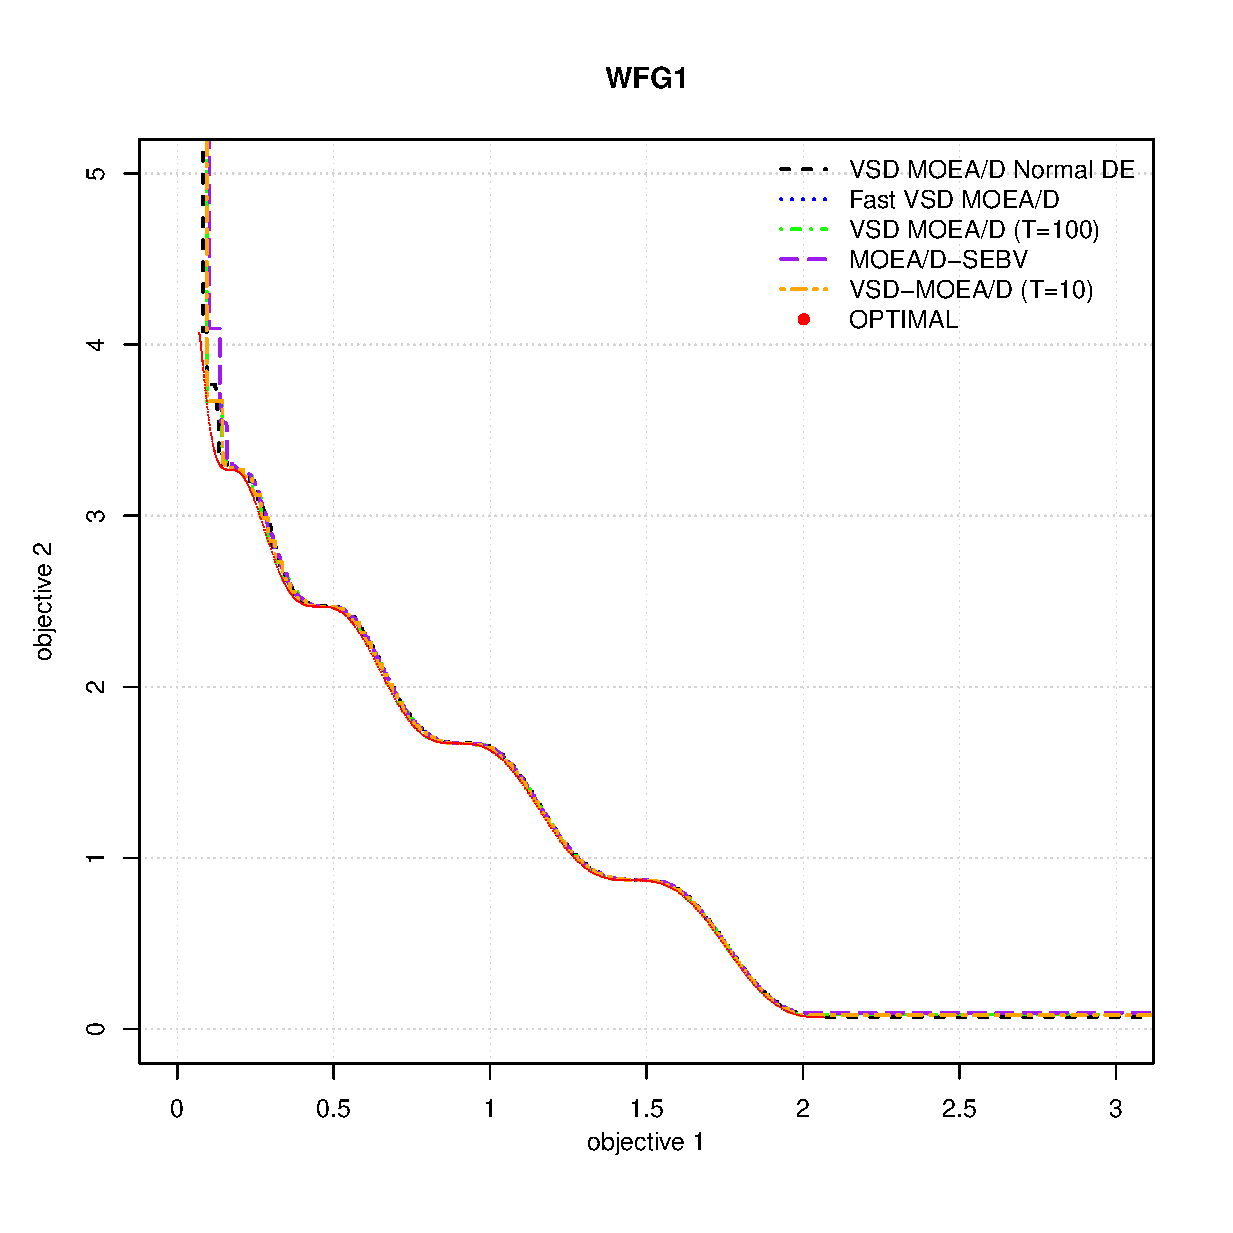
\includegraphics[width=0.33\textwidth]{Figures_Chapter7/Results_Chapter4/Surface_eps_VSD_MOEA/WFG1.eps}  &
  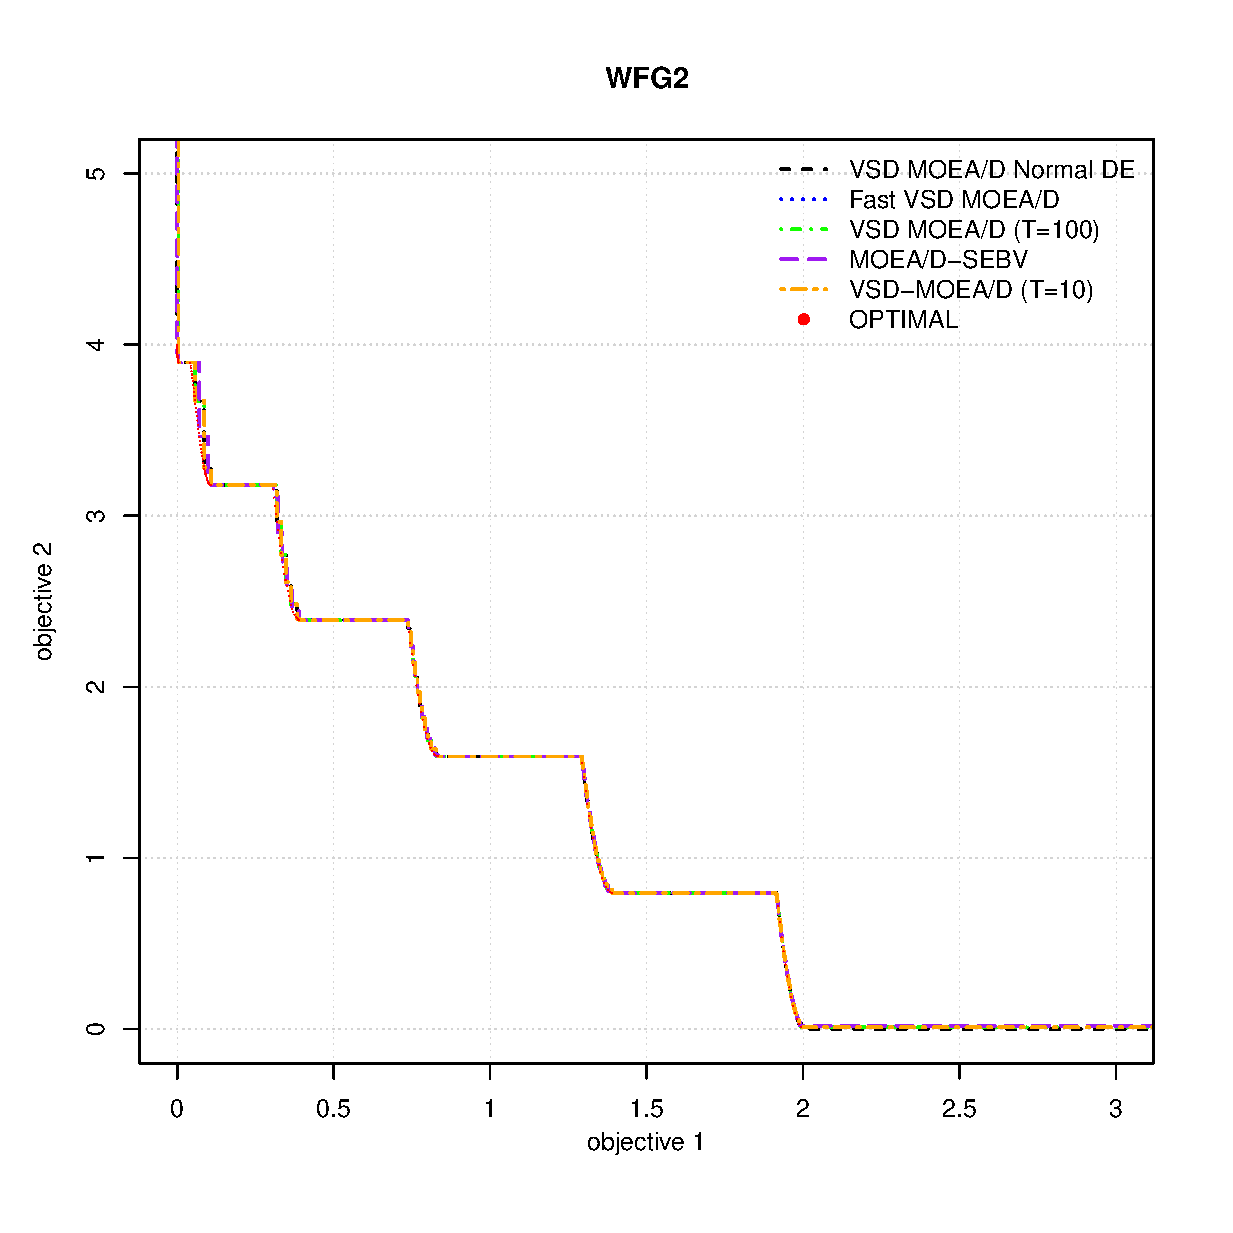
\includegraphics[width=0.33\textwidth]{Figures_Chapter7/Results_Chapter4/Surface_eps_VSD_MOEA/WFG2.eps} &
  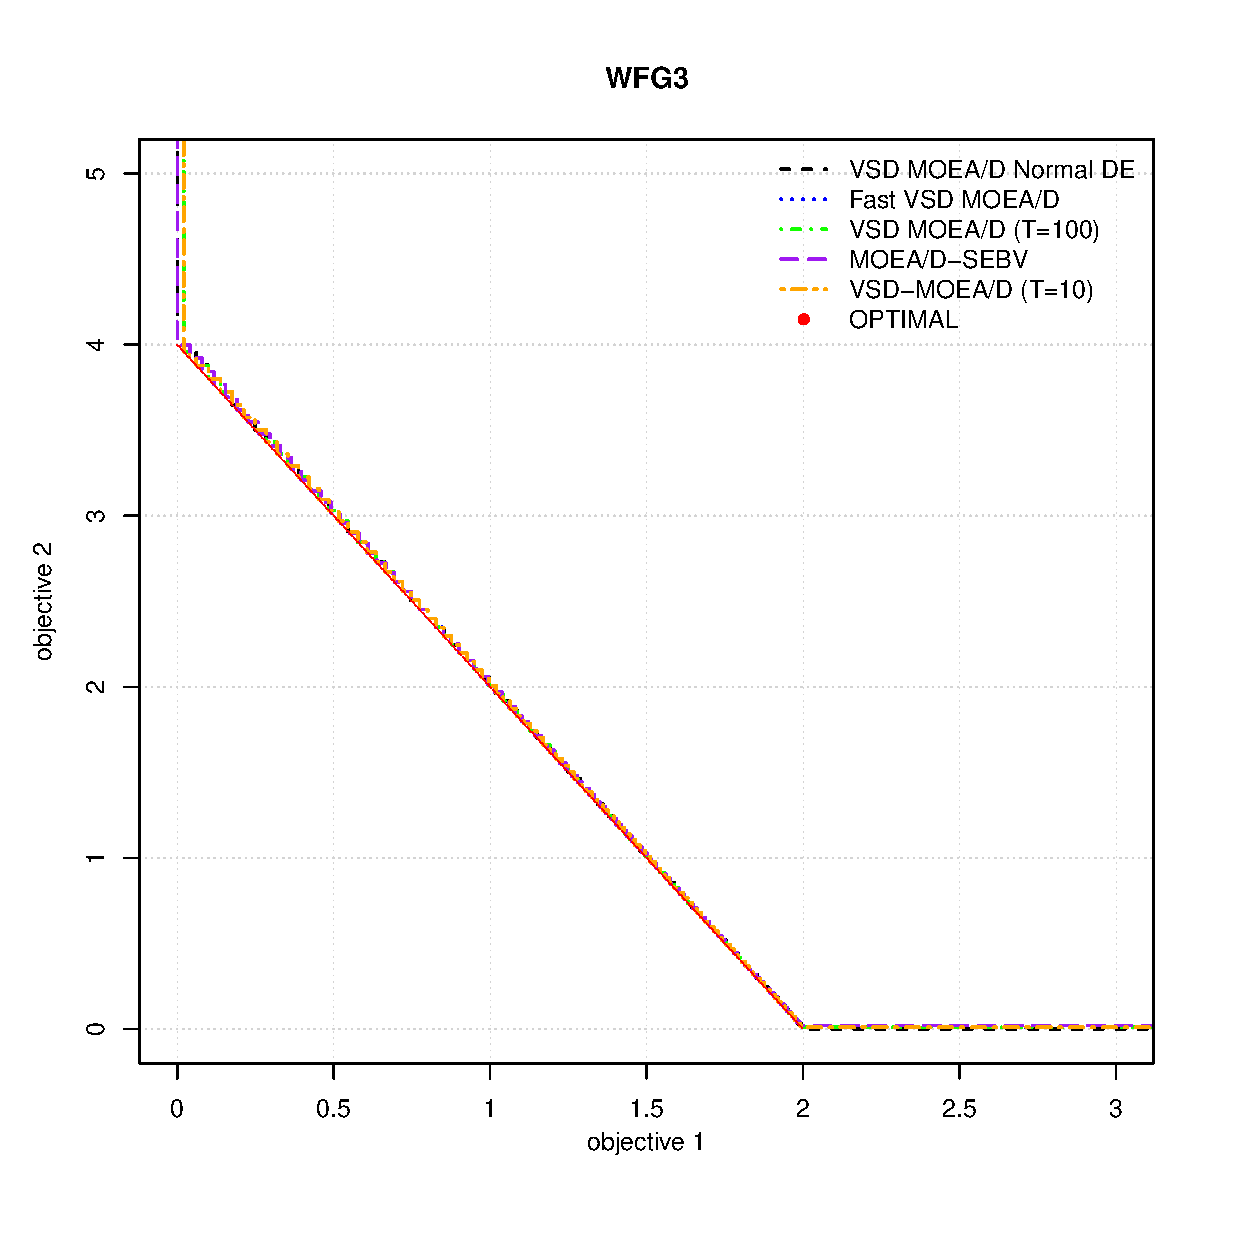
\includegraphics[width=0.33\textwidth]{Figures_Chapter7/Results_Chapter4/Surface_eps_VSD_MOEA/WFG3.eps} \\
  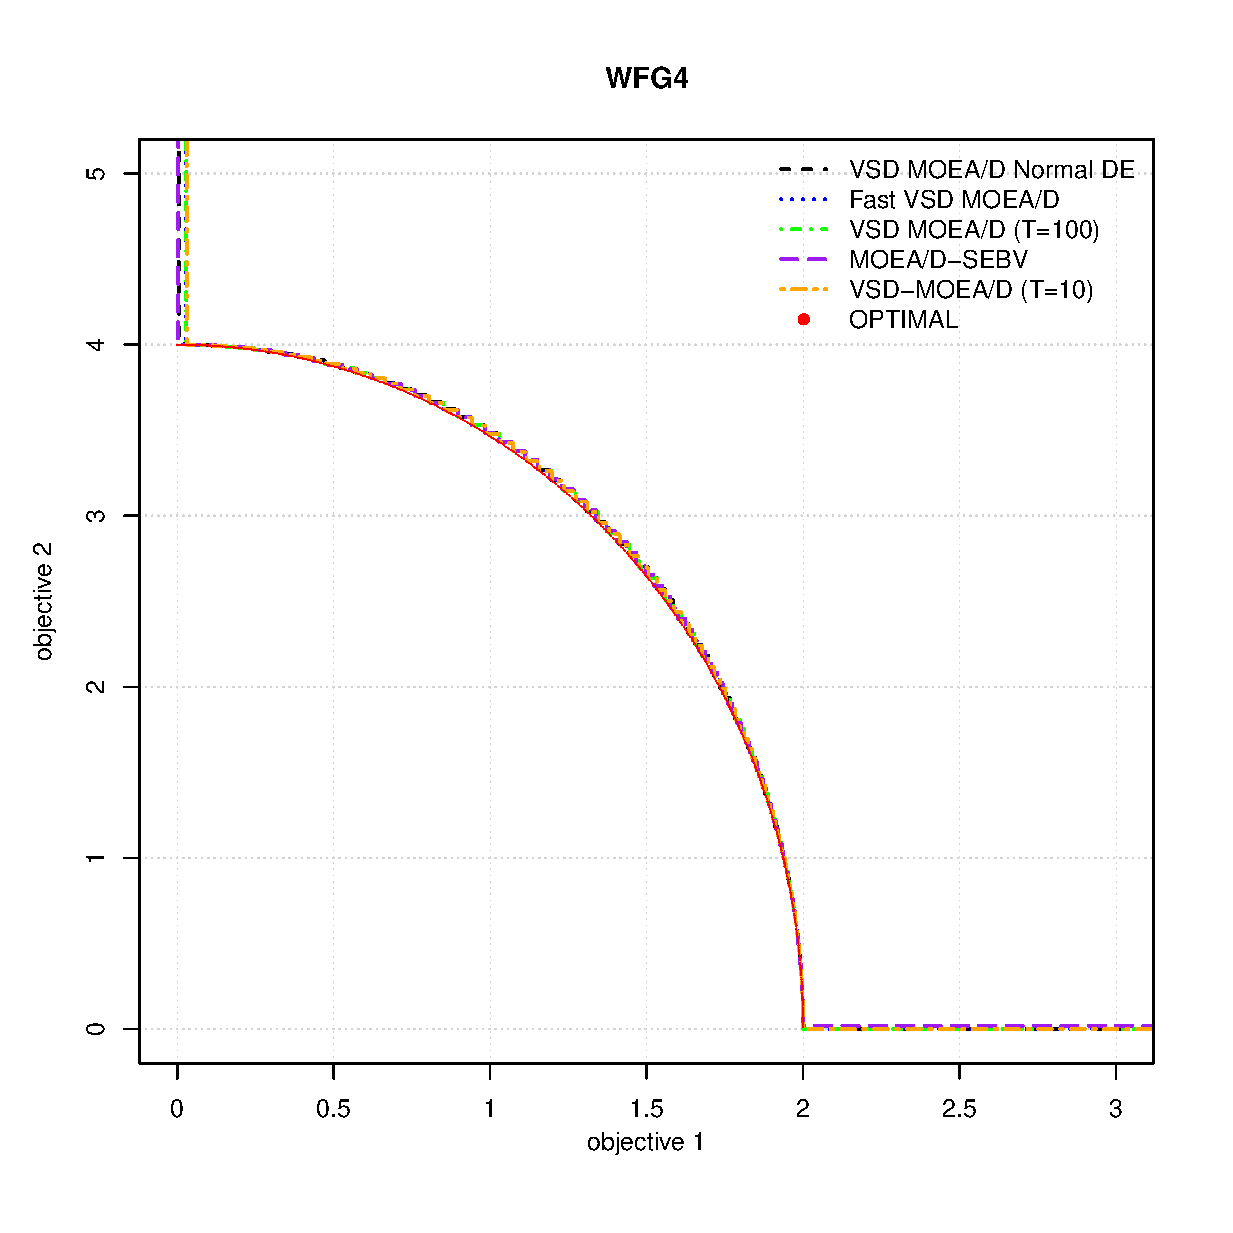
\includegraphics[width=0.33\textwidth]{Figures_Chapter7/Results_Chapter4/Surface_eps_VSD_MOEA/WFG4.eps} &
  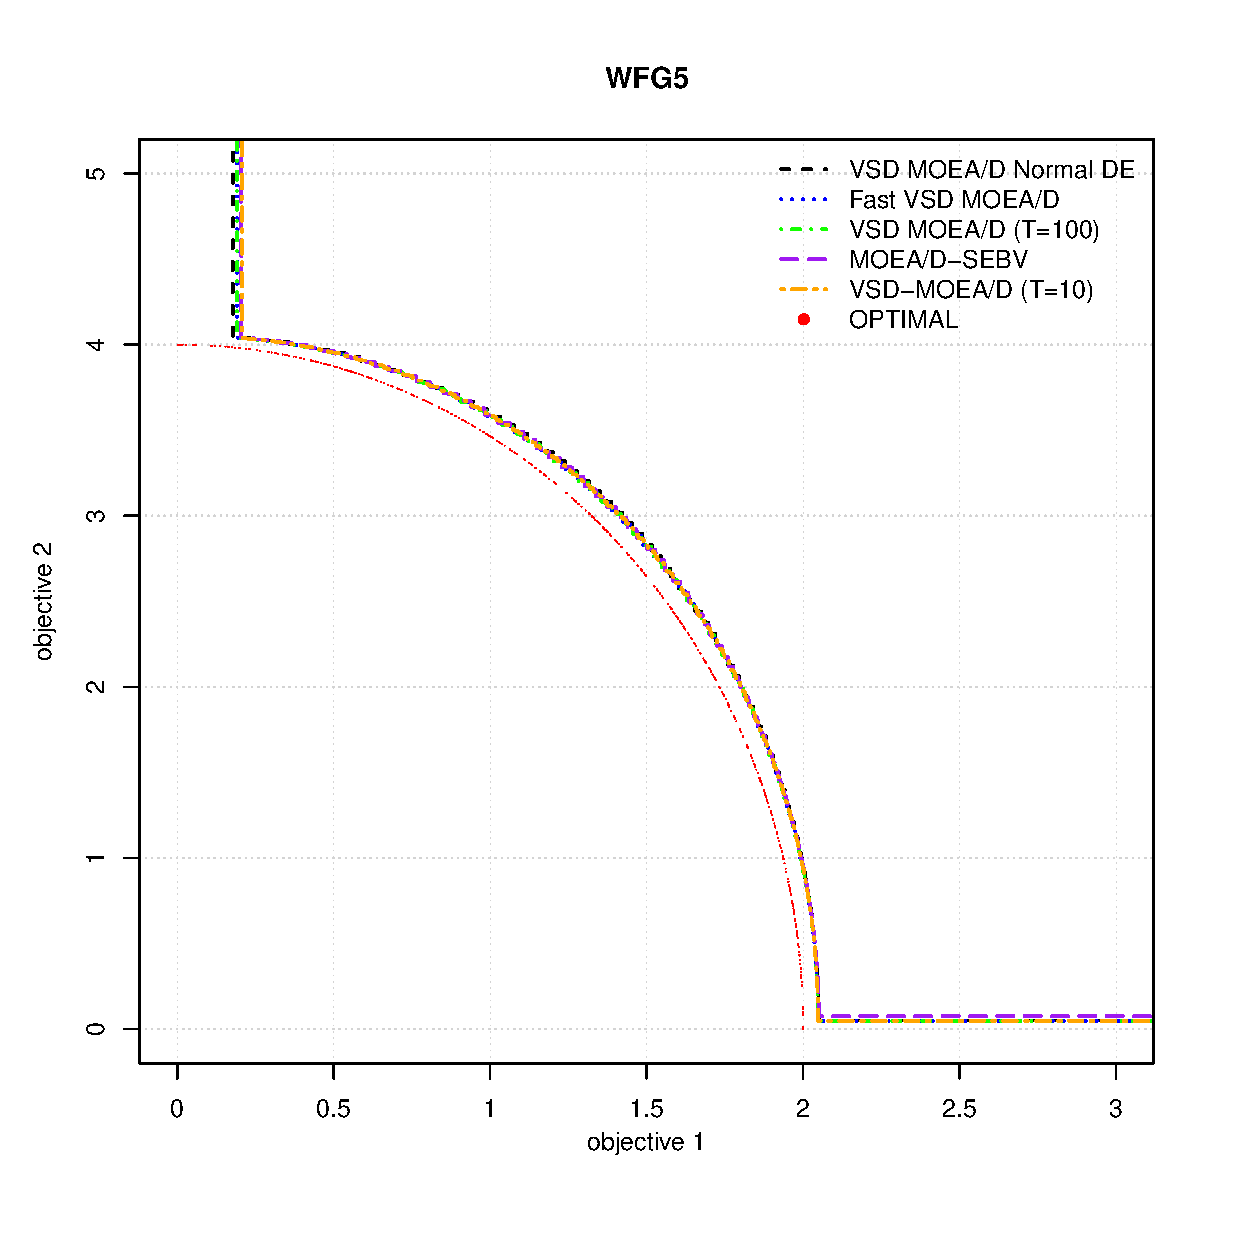
\includegraphics[width=0.33\textwidth]{Figures_Chapter7/Results_Chapter4/Surface_eps_VSD_MOEA/WFG5.eps} &
  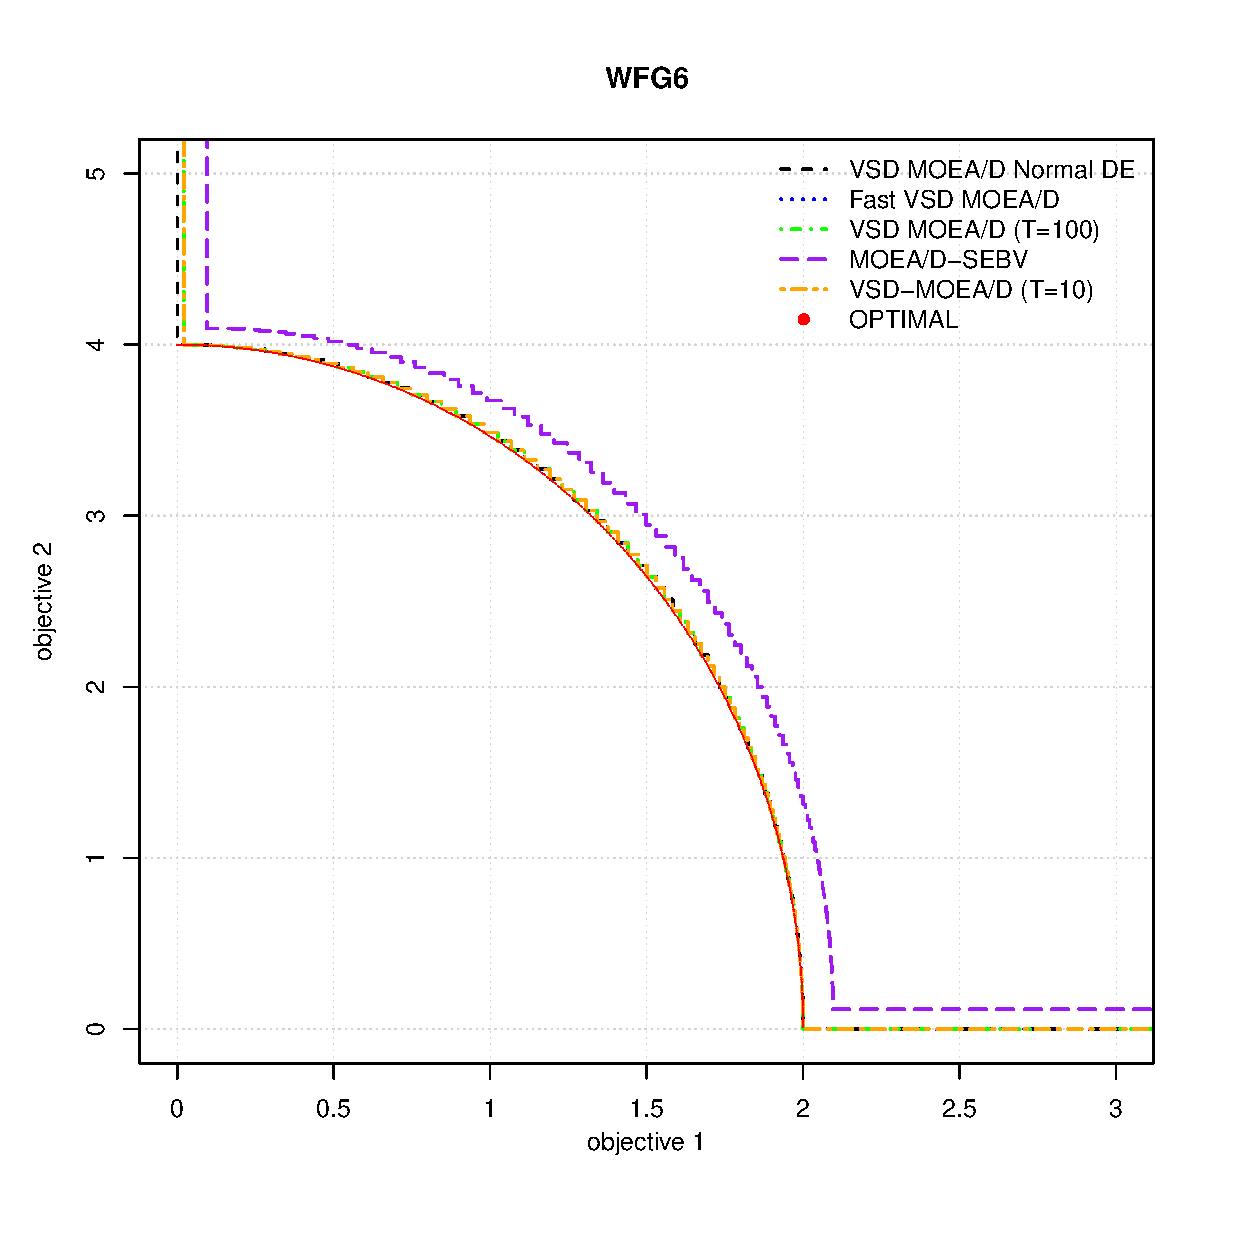
\includegraphics[width=0.33\textwidth]{Figures_Chapter7/Results_Chapter4/Surface_eps_VSD_MOEA/WFG6.eps} \\
  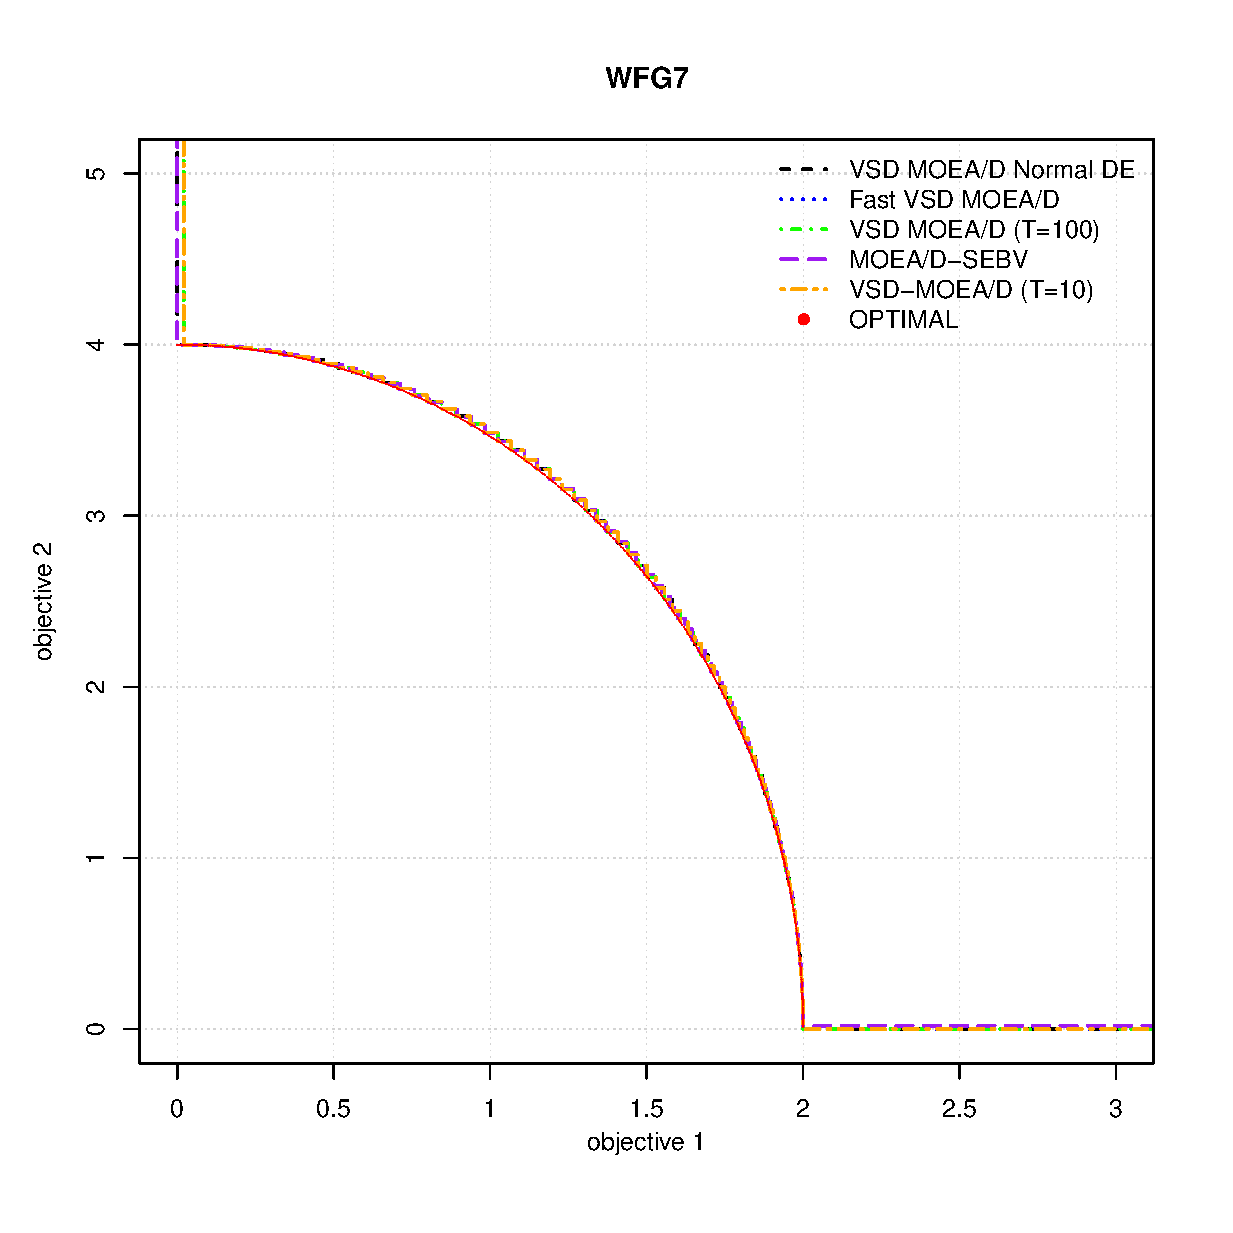
\includegraphics[width=0.33\textwidth]{Figures_Chapter7/Results_Chapter4/Surface_eps_VSD_MOEA/WFG7.eps} &
  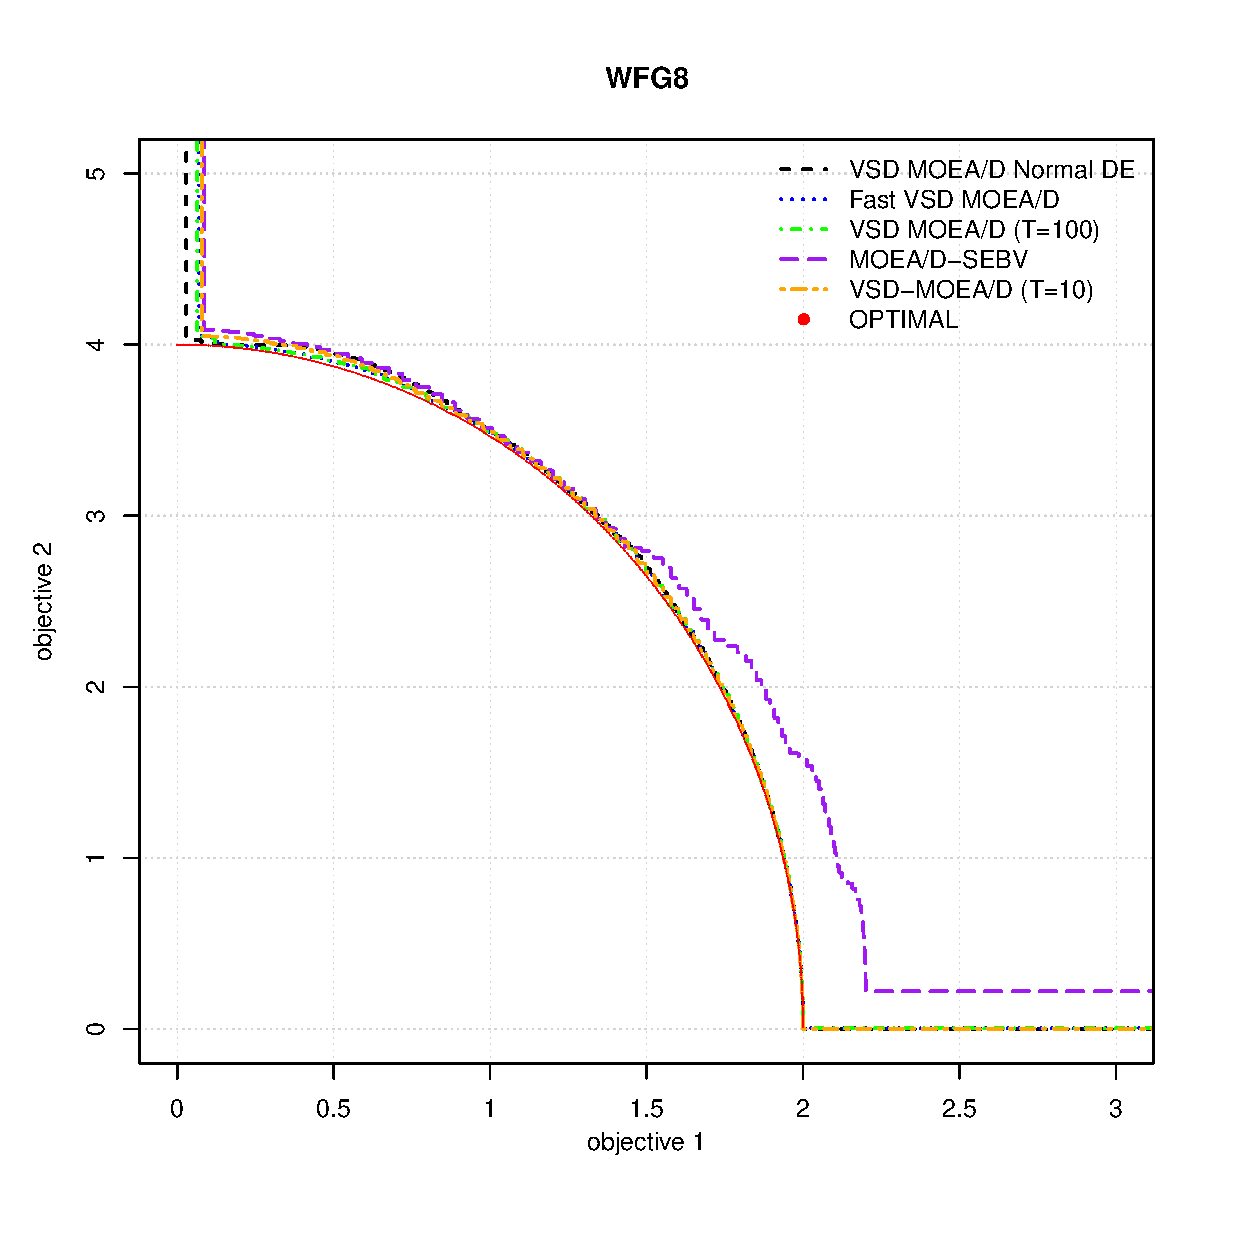
\includegraphics[width=0.33\textwidth]{Figures_Chapter7/Results_Chapter4/Surface_eps_VSD_MOEA/WFG8.eps} &
  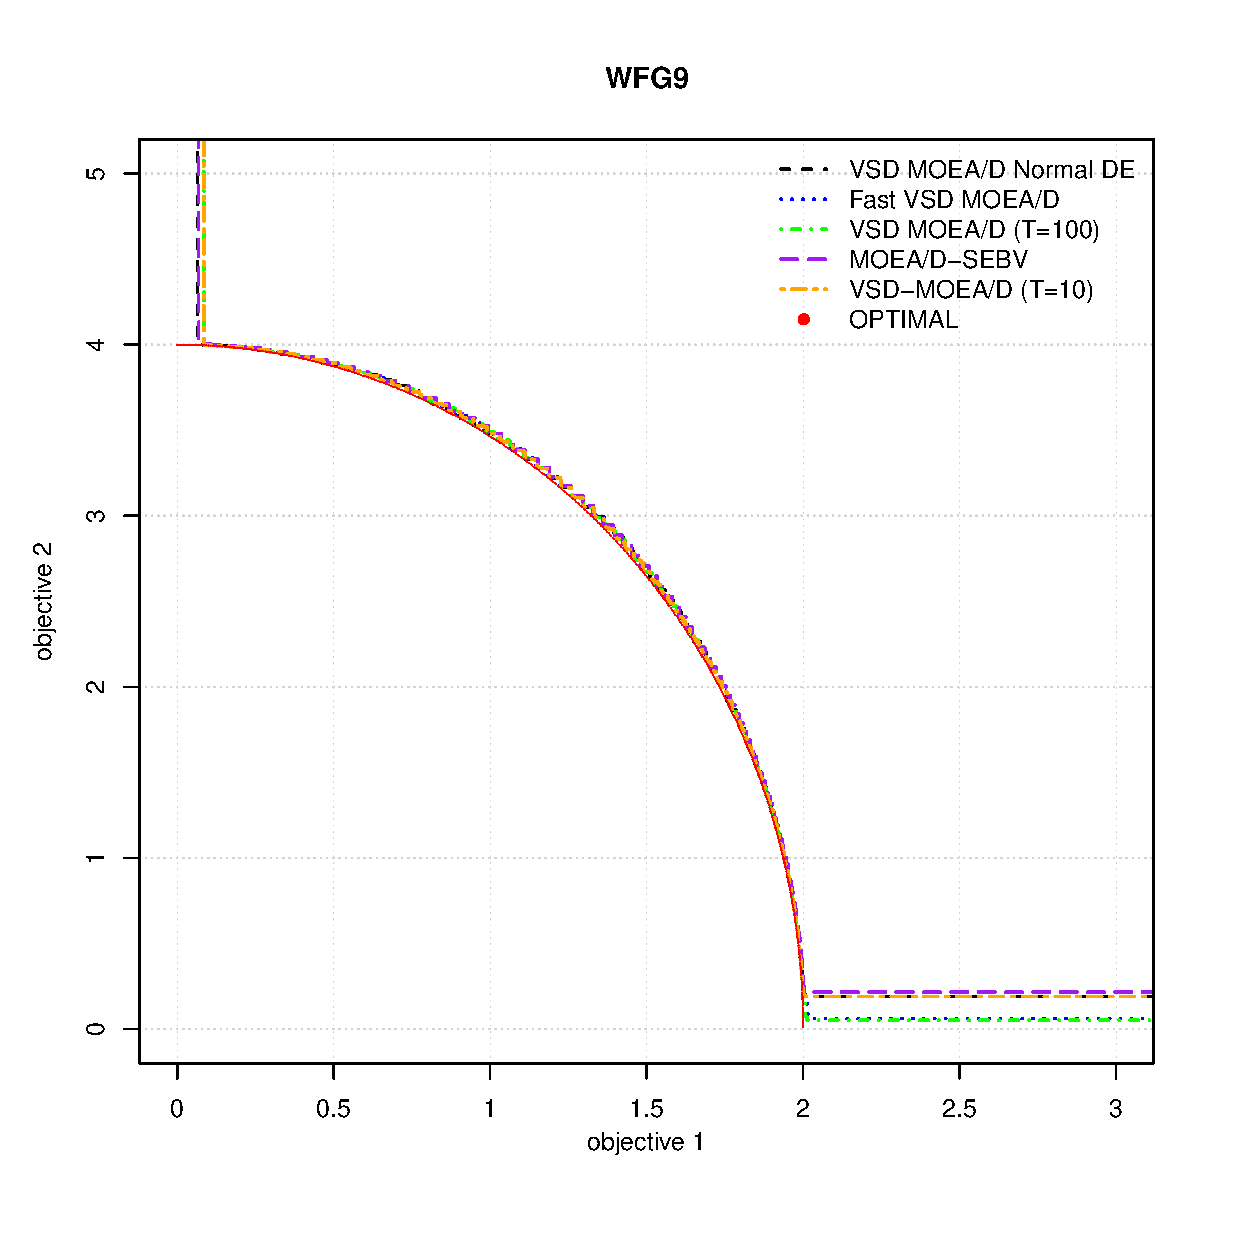
\includegraphics[width=0.33\textwidth]{Figures_Chapter7/Results_Chapter4/Surface_eps_VSD_MOEA/WFG9.eps}
\end{tabular}
\end{figure}
\begin{figure}[H]
%%\centering
\caption{superficies de cubrimiento logradas al 50\%}%Attainment Figures\_Chapter7 Achieved}
\begin{tabular}{ccc}
  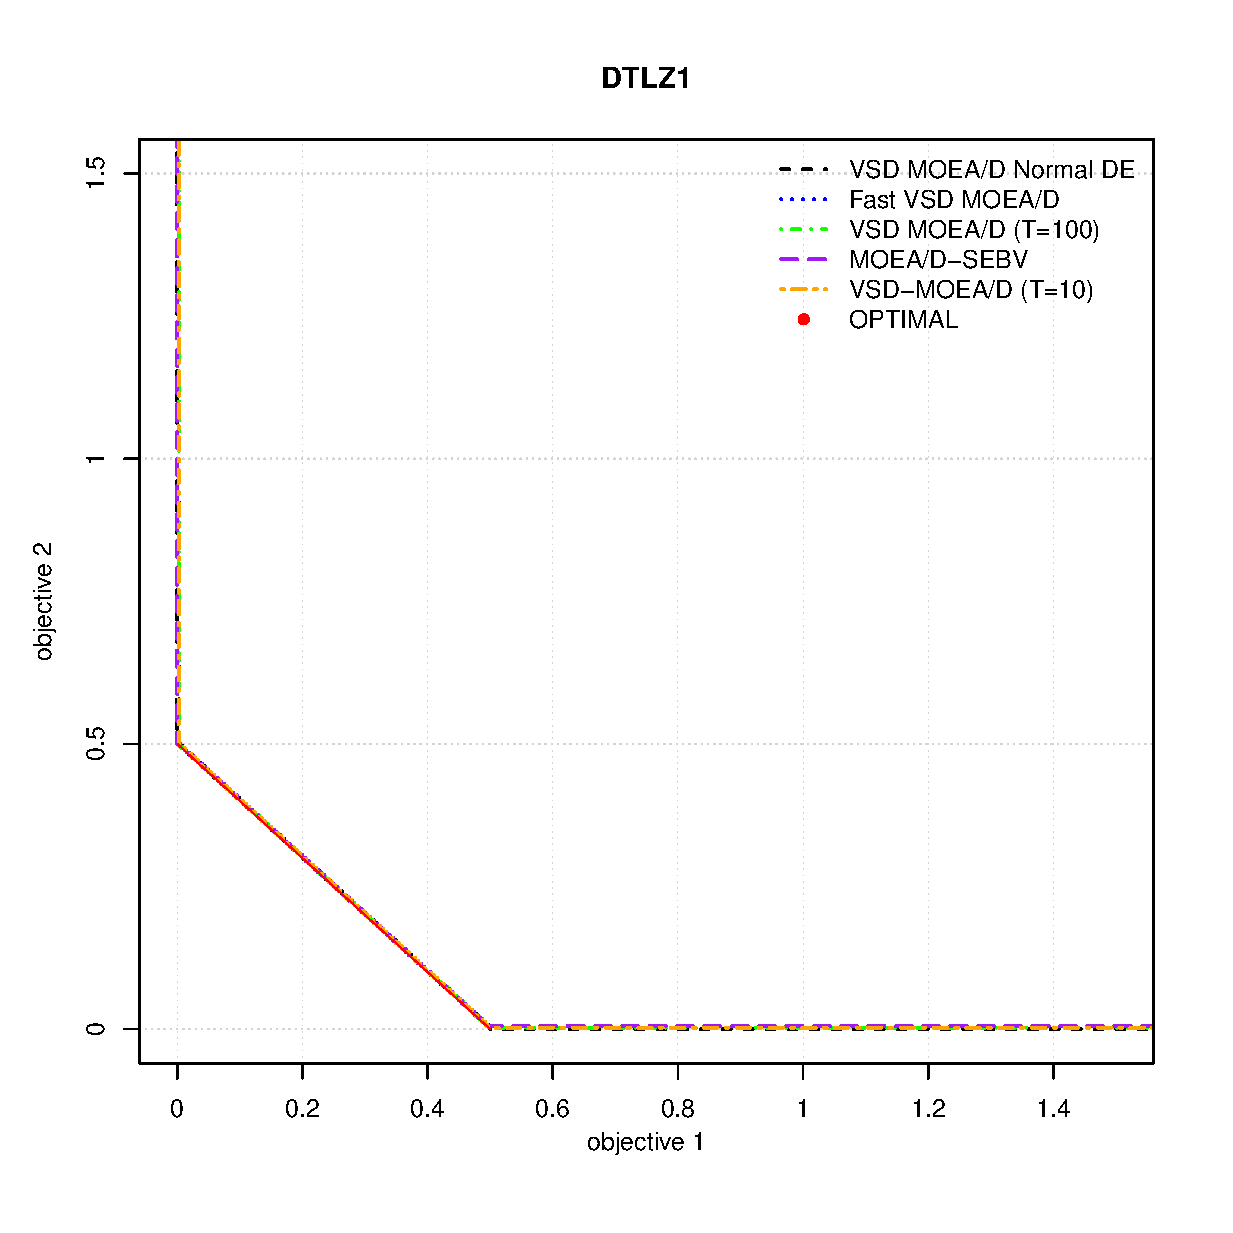
\includegraphics[width=0.33\textwidth]{Figures_Chapter7/Results_Chapter4/Surface_eps_VSD_MOEA/DTLZ1.eps}  &
  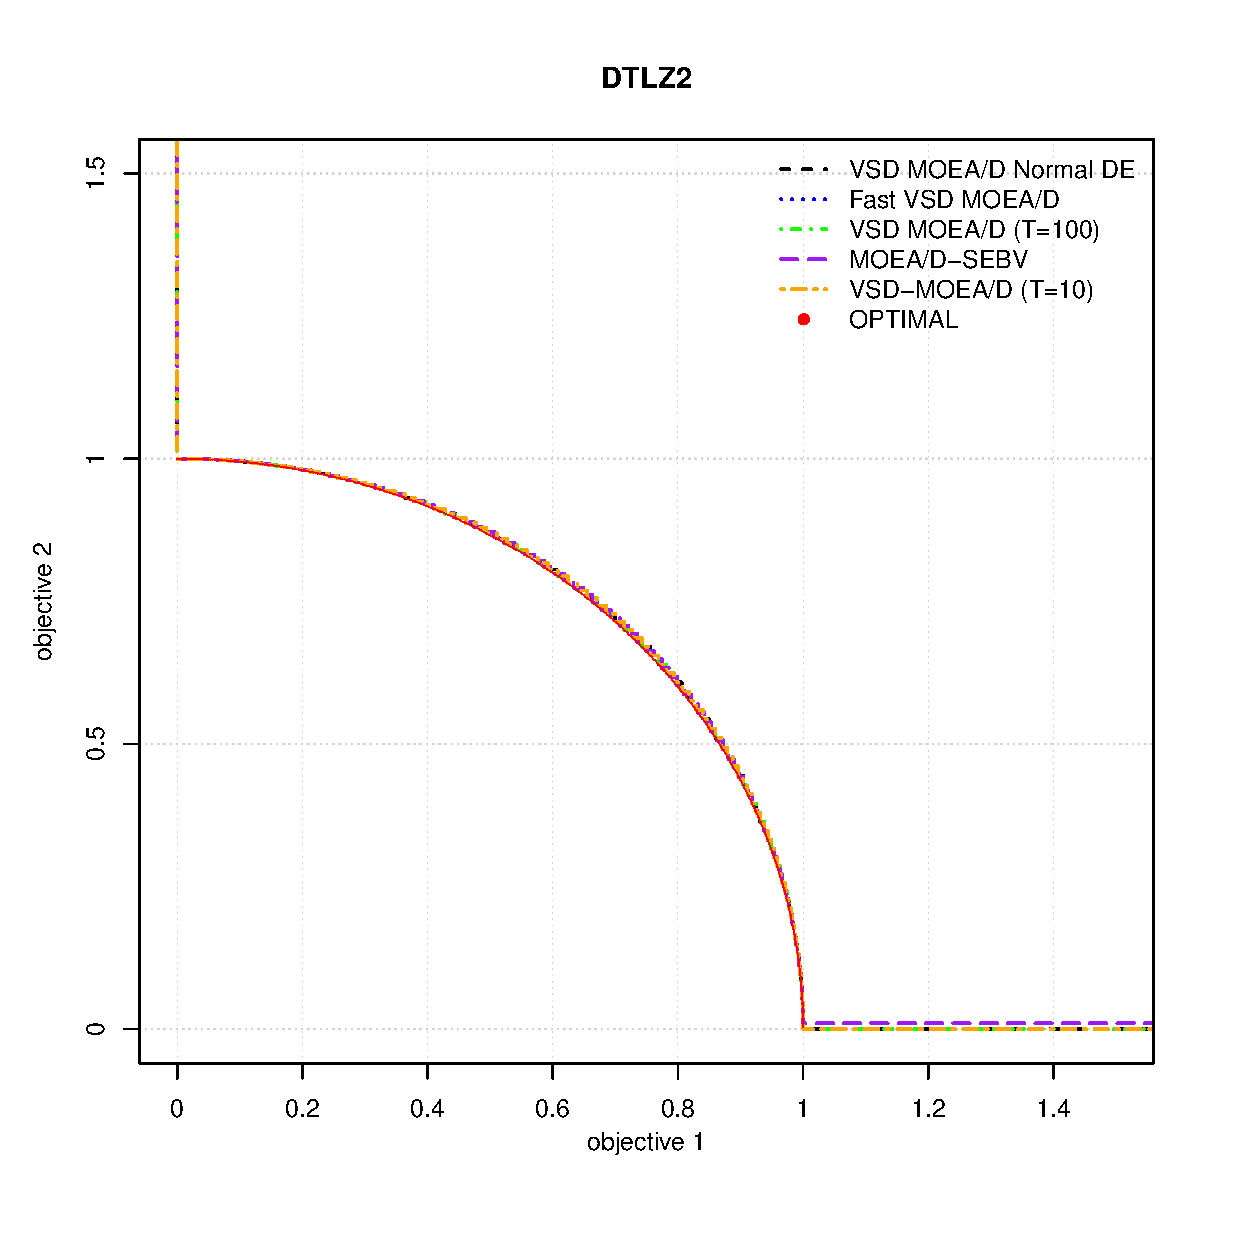
\includegraphics[width=0.33\textwidth]{Figures_Chapter7/Results_Chapter4/Surface_eps_VSD_MOEA/DTLZ2.eps} &
  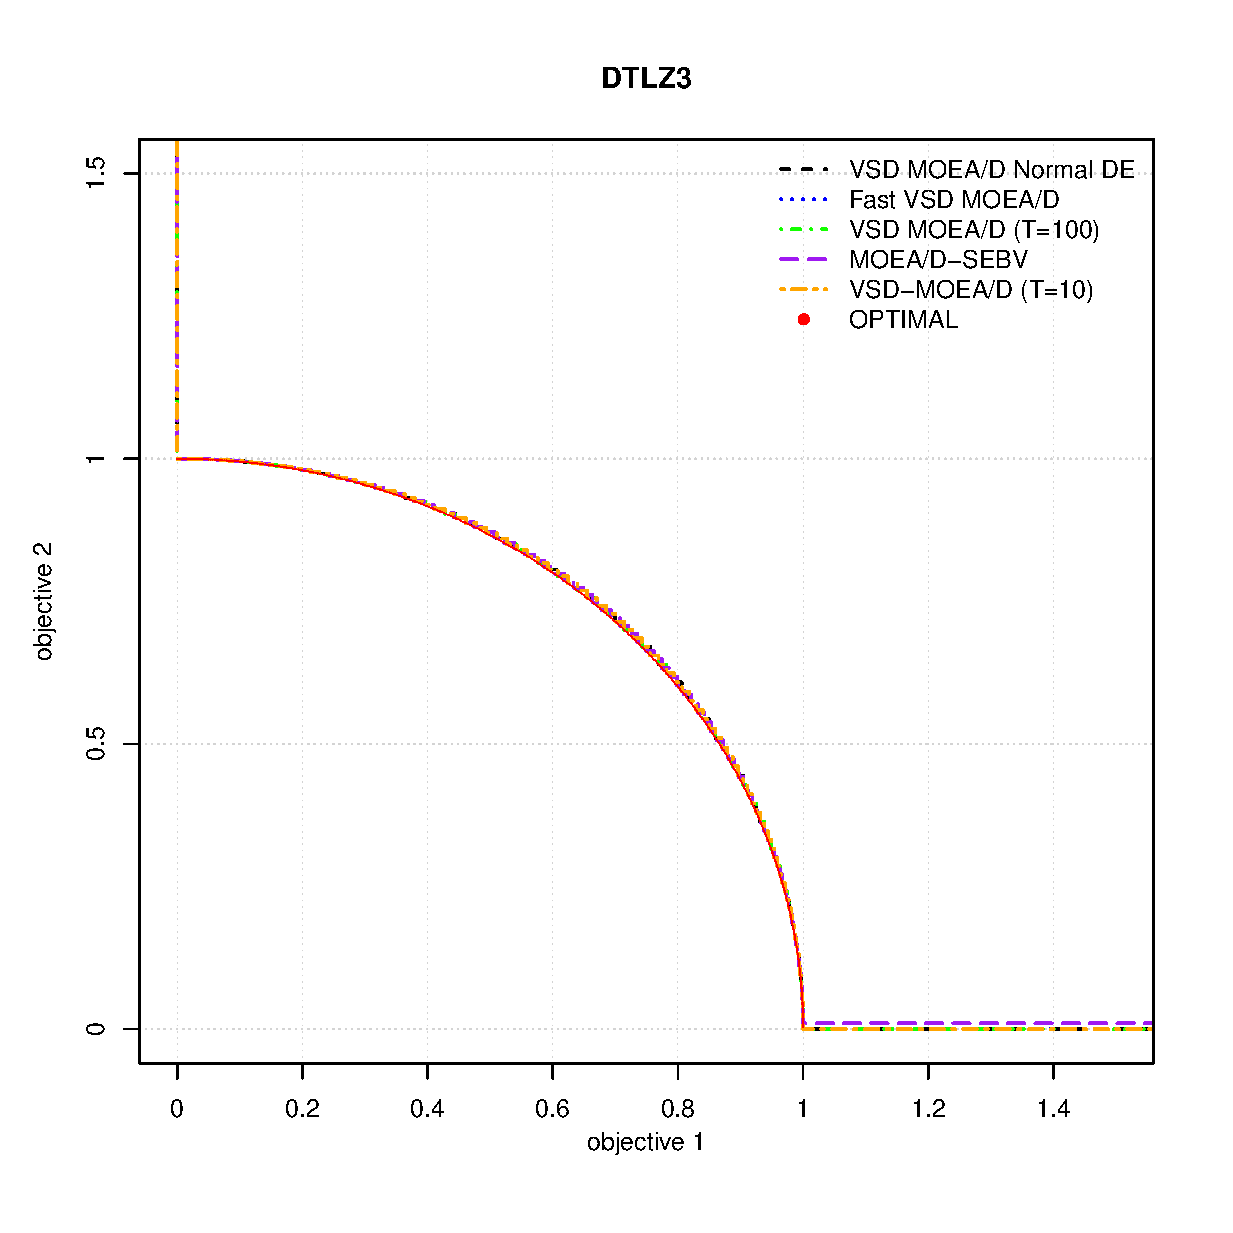
\includegraphics[width=0.33\textwidth]{Figures_Chapter7/Results_Chapter4/Surface_eps_VSD_MOEA/DTLZ3.eps} \\
  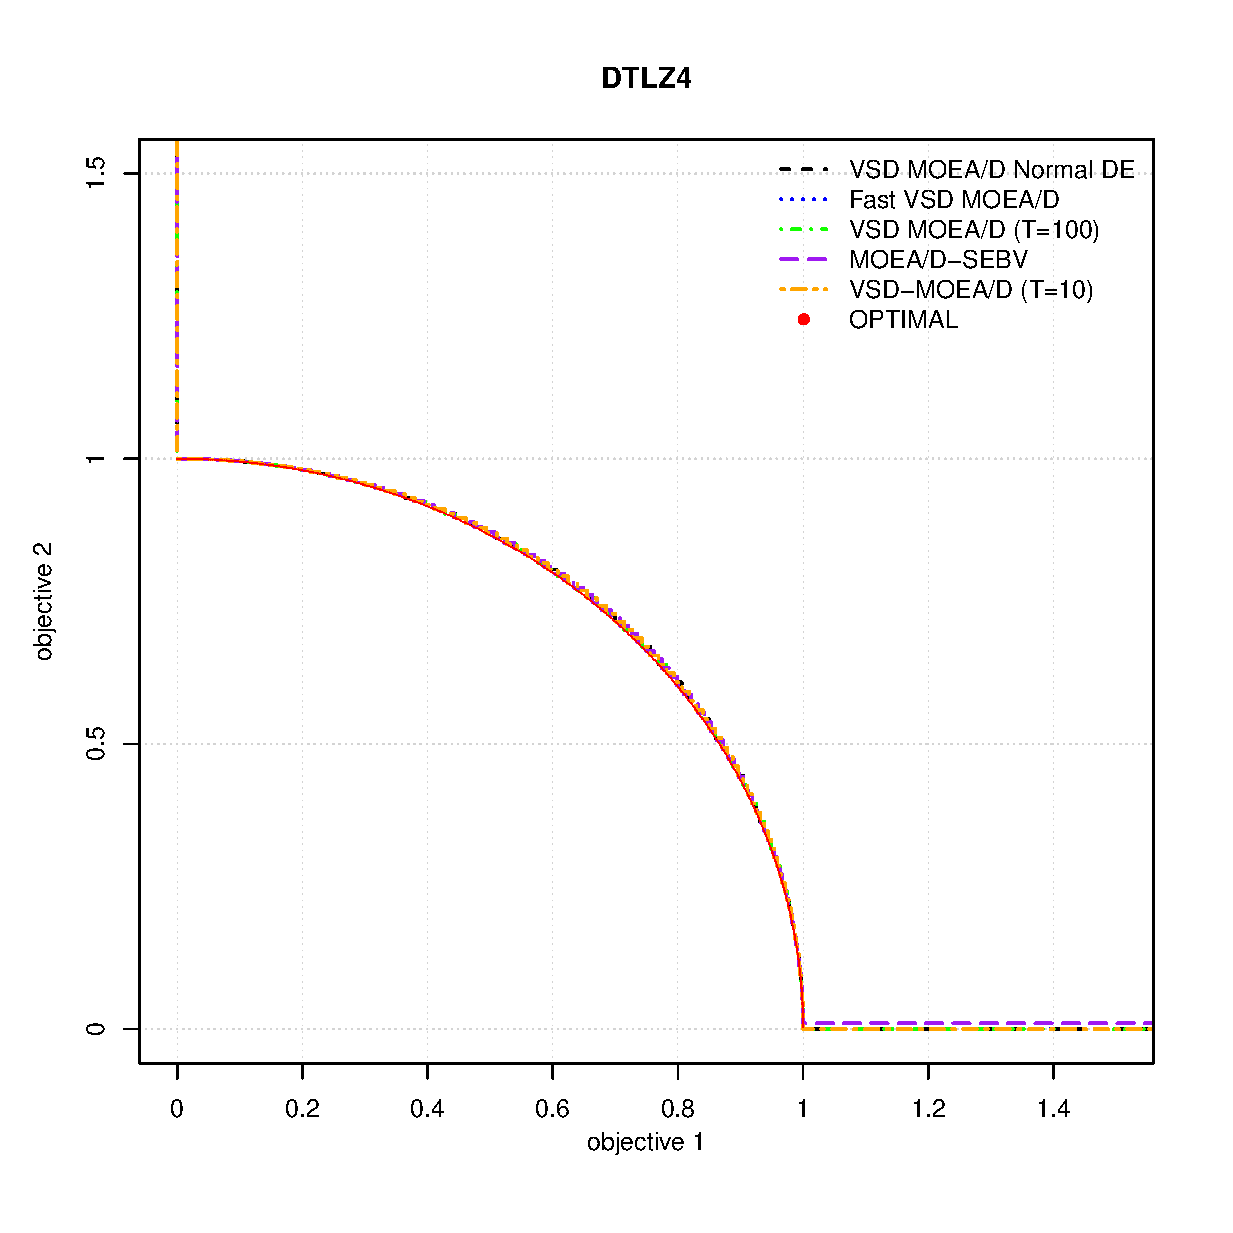
\includegraphics[width=0.33\textwidth]{Figures_Chapter7/Results_Chapter4/Surface_eps_VSD_MOEA/DTLZ4.eps} &
  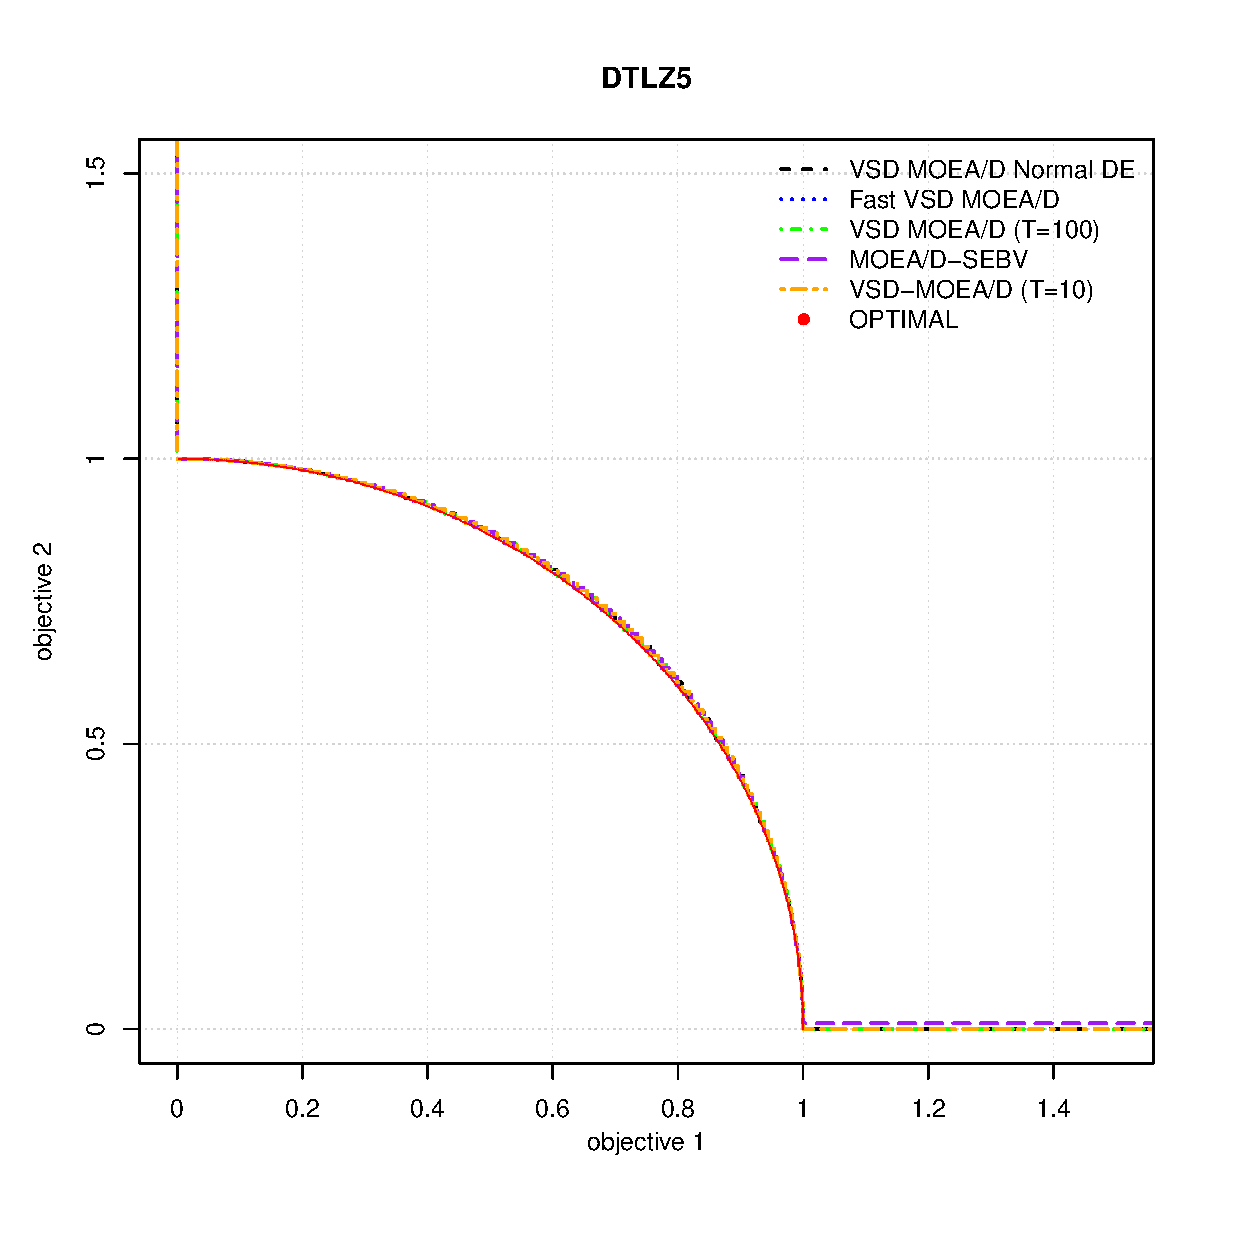
\includegraphics[width=0.33\textwidth]{Figures_Chapter7/Results_Chapter4/Surface_eps_VSD_MOEA/DTLZ5.eps} &
  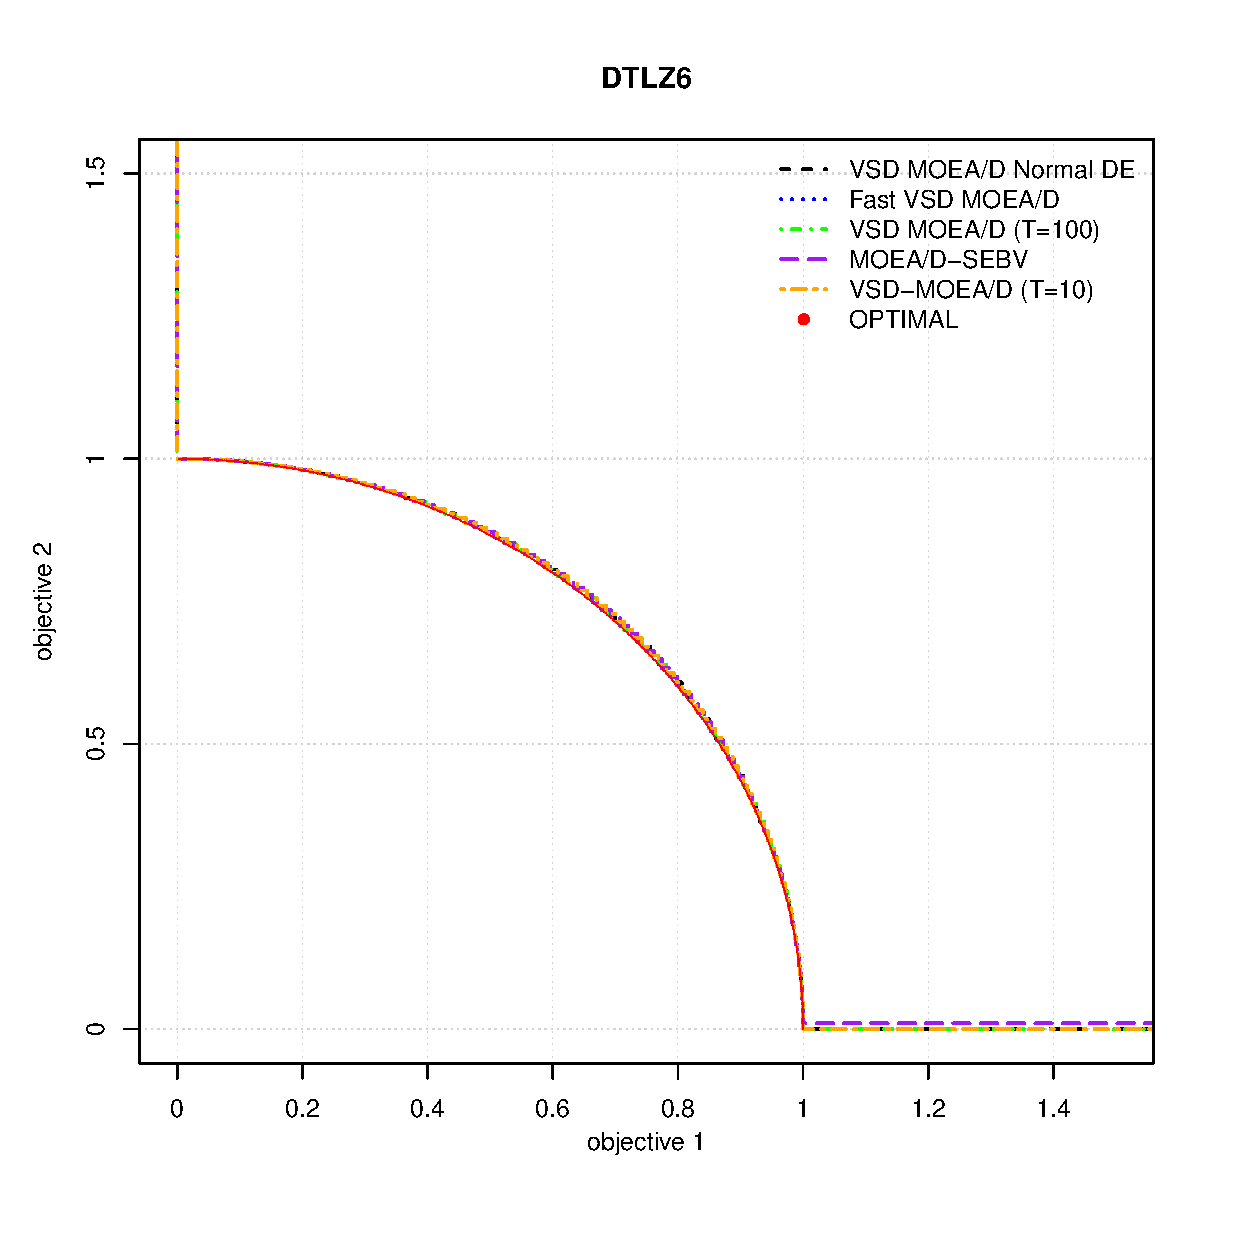
\includegraphics[width=0.33\textwidth]{Figures_Chapter7/Results_Chapter4/Surface_eps_VSD_MOEA/DTLZ6.eps} \\
  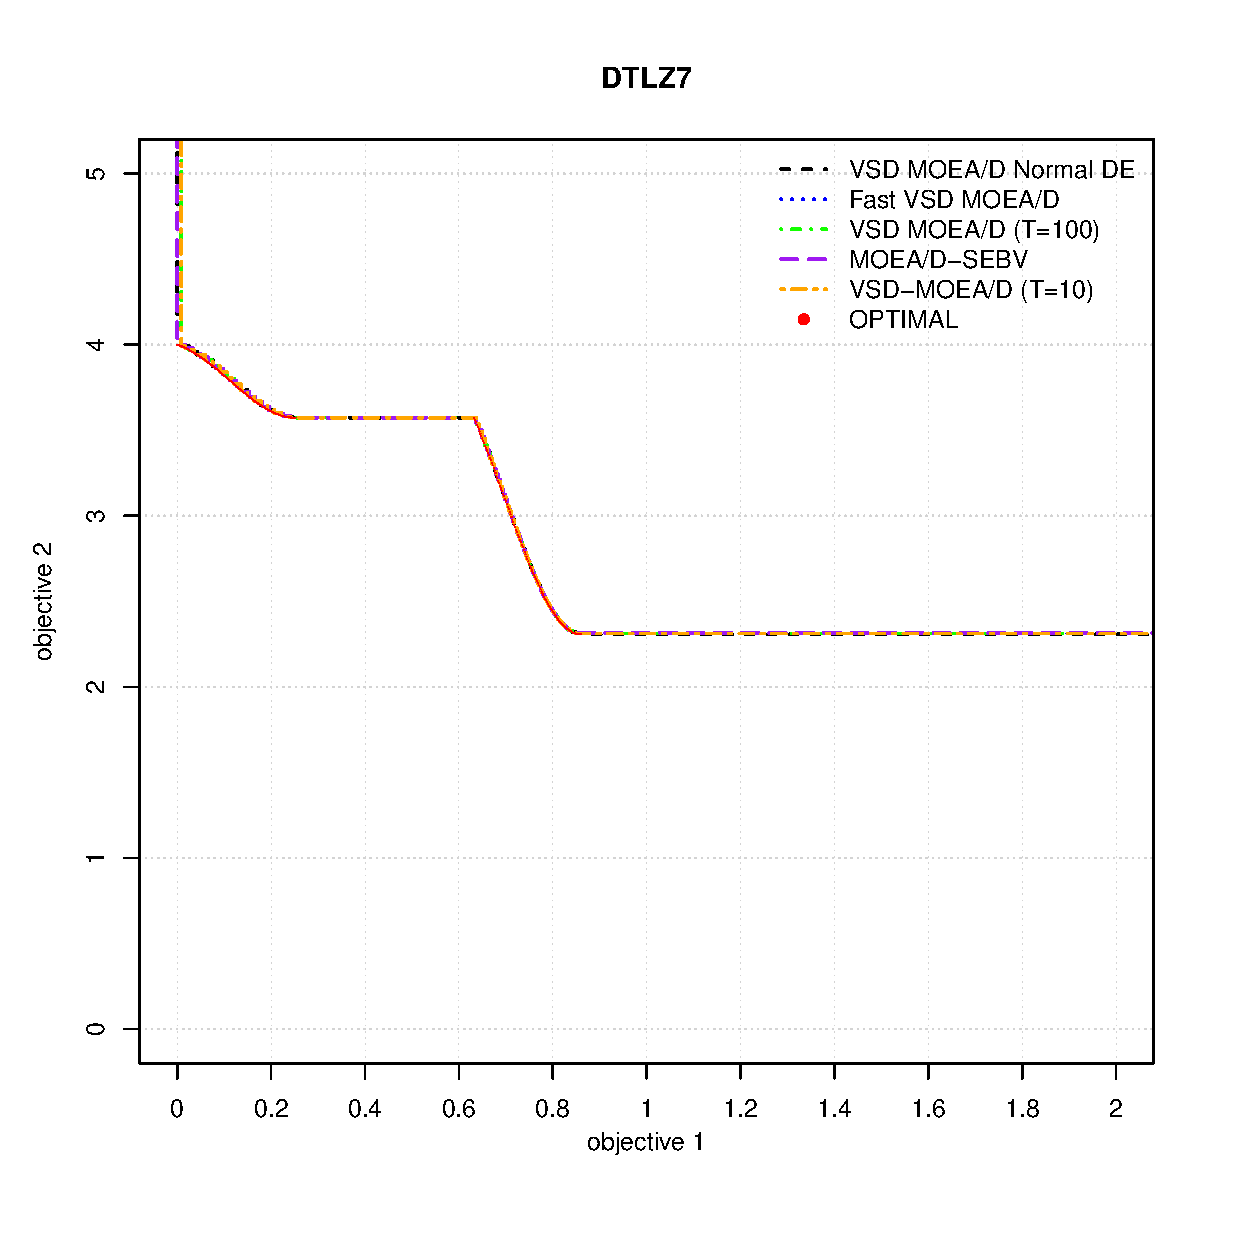
\includegraphics[width=0.33\textwidth]{Figures_Chapter7/Results_Chapter4/Surface_eps_VSD_MOEA/DTLZ7.eps} 
\end{tabular}
\end{figure}

\begin{figure}[H]
%%\centering
\caption{superficies de cubrimiento logradas al 50\%}%Attainment Figures\_Chapter7 Achieved}
\begin{tabular}{ccc}
  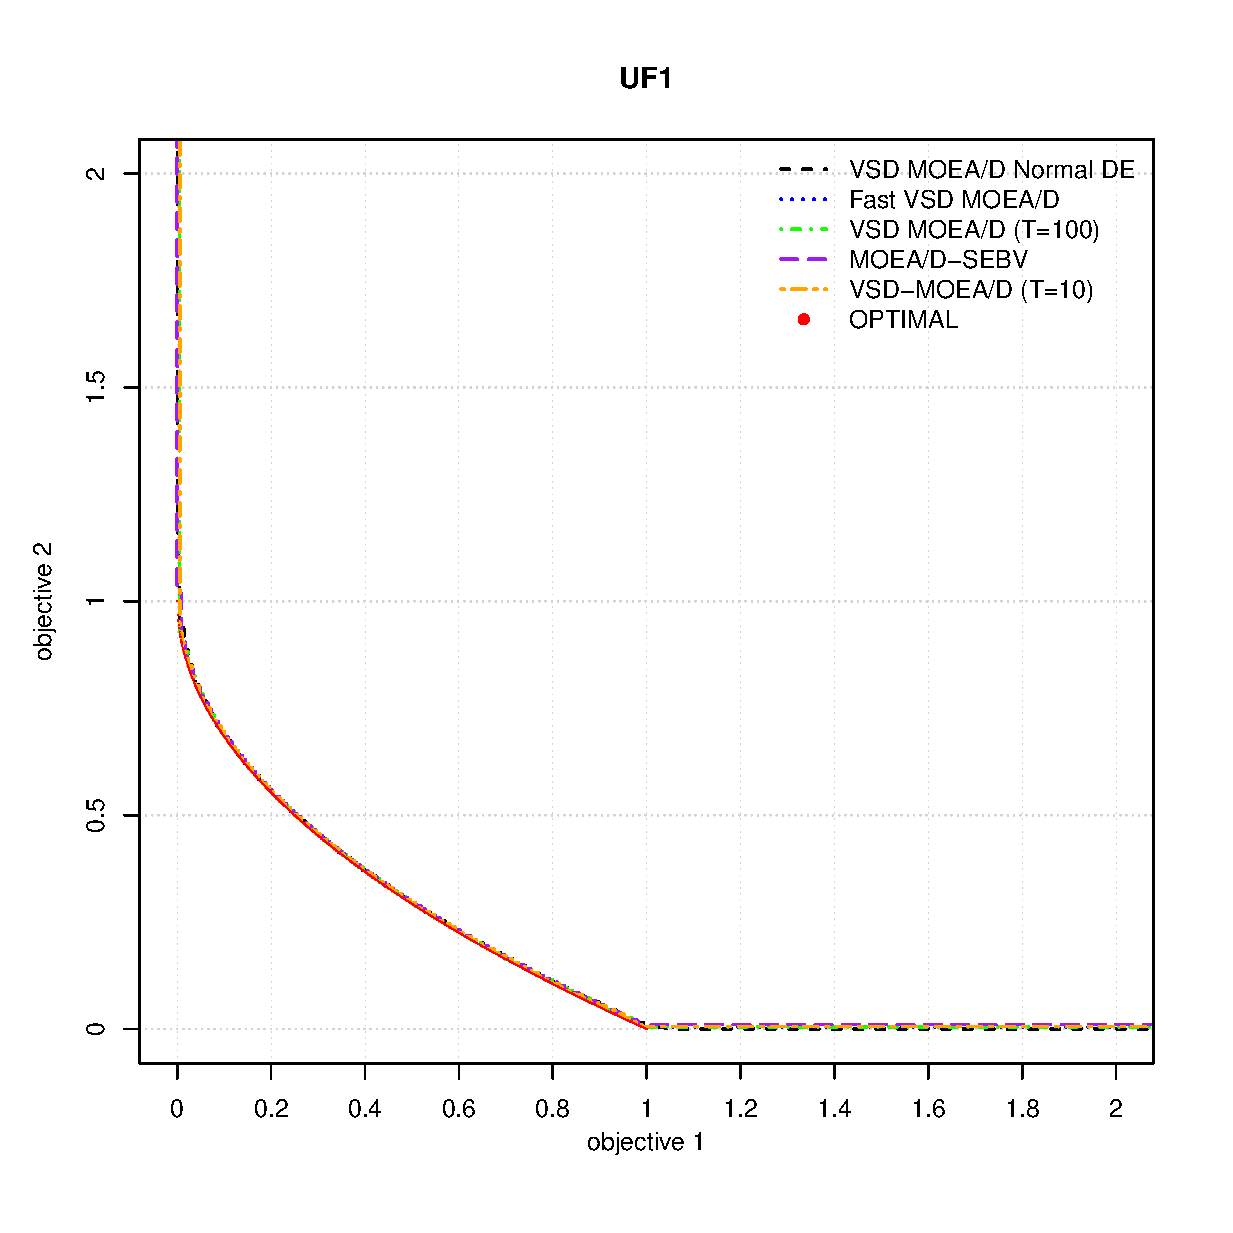
\includegraphics[width=0.33\textwidth]{Figures_Chapter7/Results_Chapter4/Surface_eps_VSD_MOEA/UF1.eps}  &
  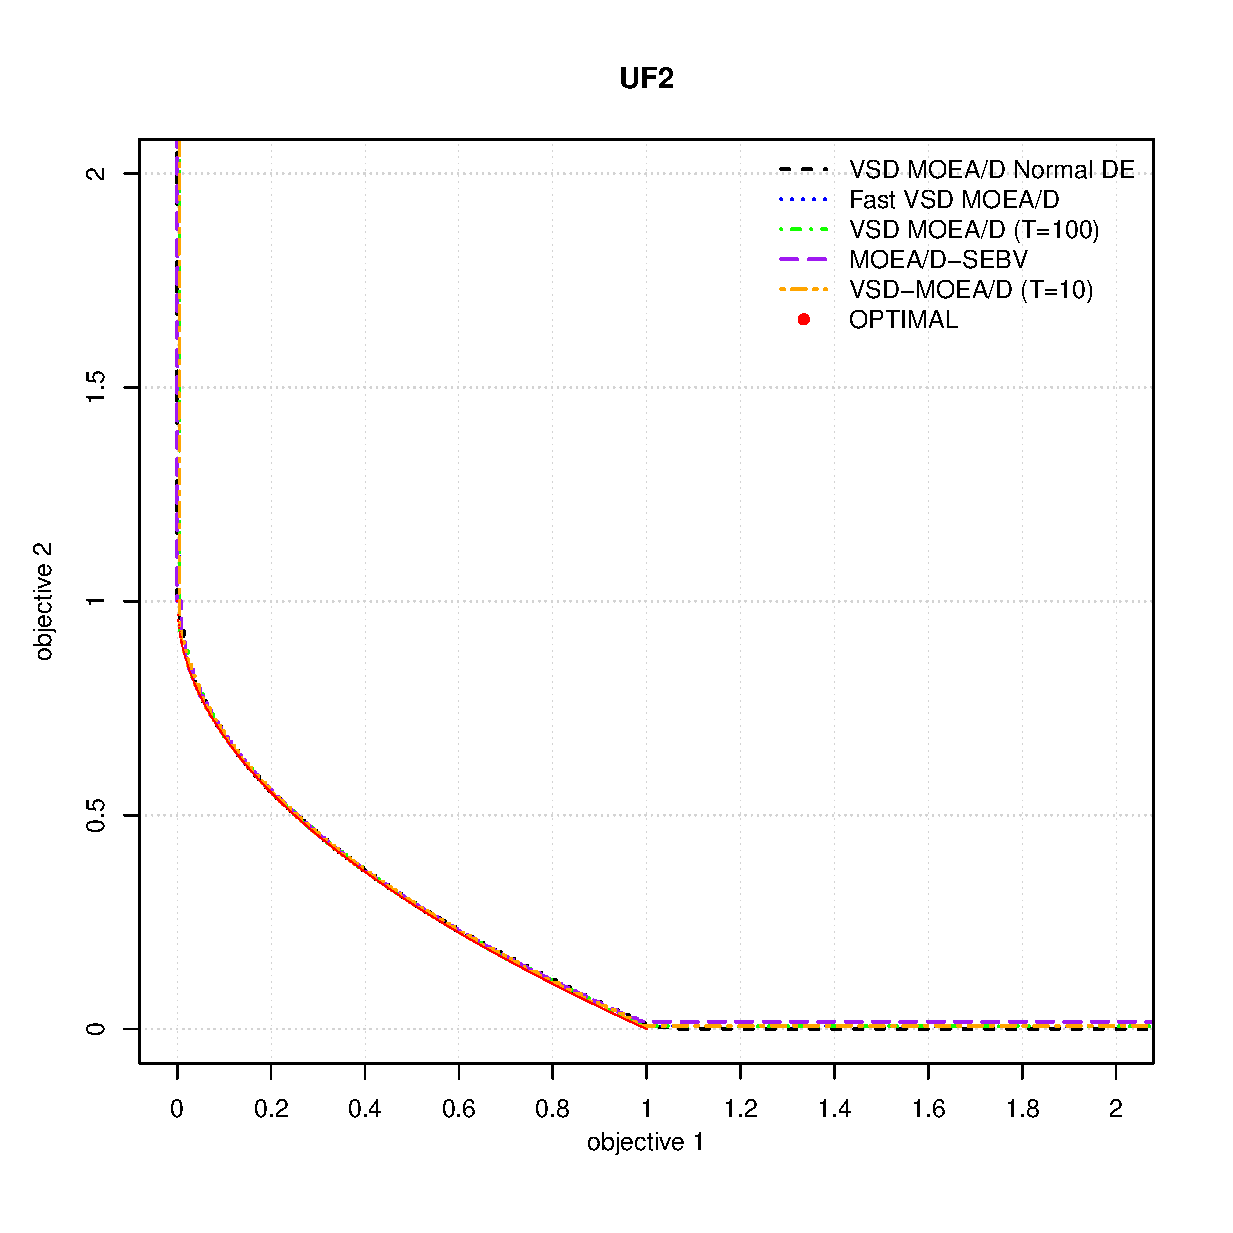
\includegraphics[width=0.33\textwidth]{Figures_Chapter7/Results_Chapter4/Surface_eps_VSD_MOEA/UF2.eps} &
  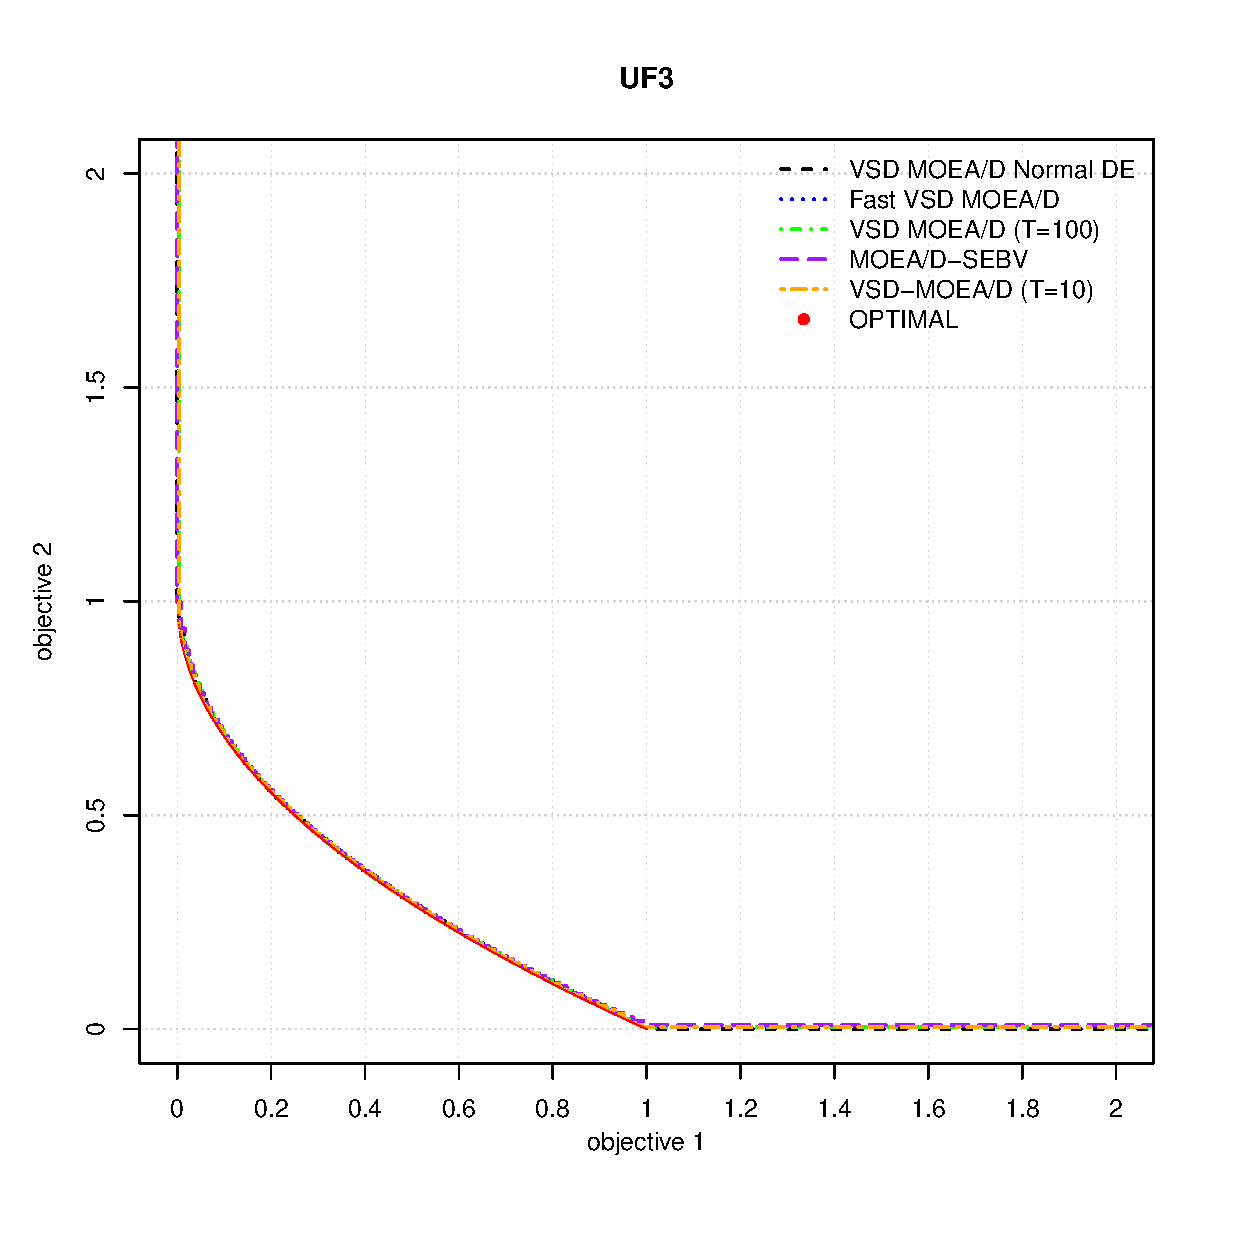
\includegraphics[width=0.33\textwidth]{Figures_Chapter7/Results_Chapter4/Surface_eps_VSD_MOEA/UF3.eps} \\
  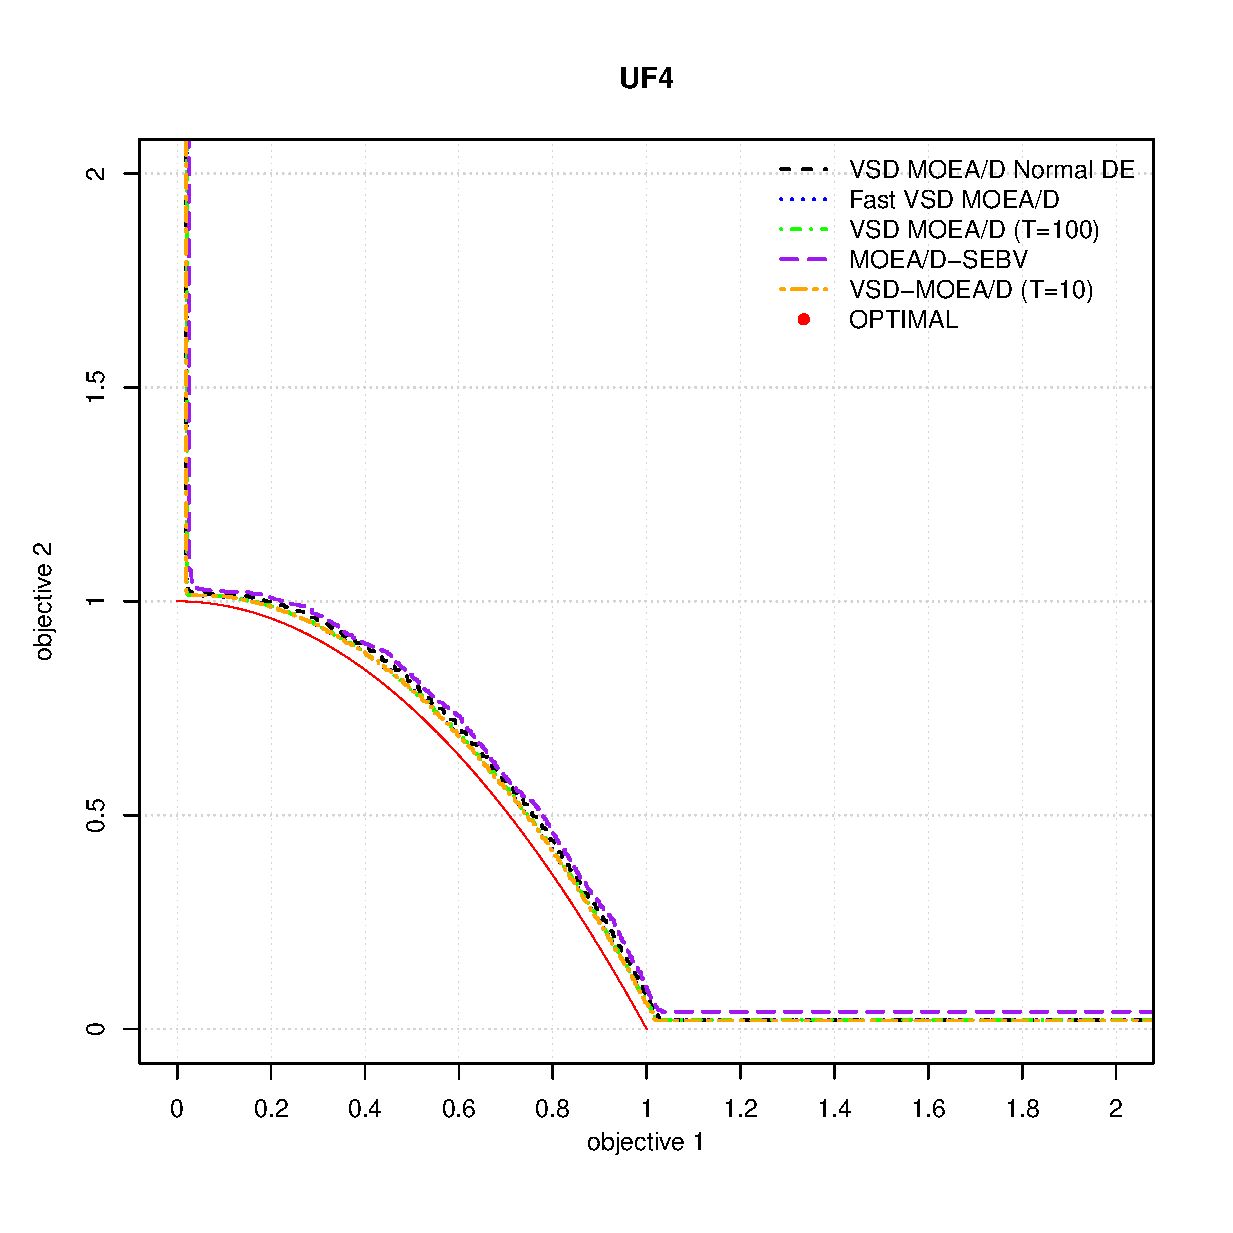
\includegraphics[width=0.33\textwidth]{Figures_Chapter7/Results_Chapter4/Surface_eps_VSD_MOEA/UF4.eps} &
  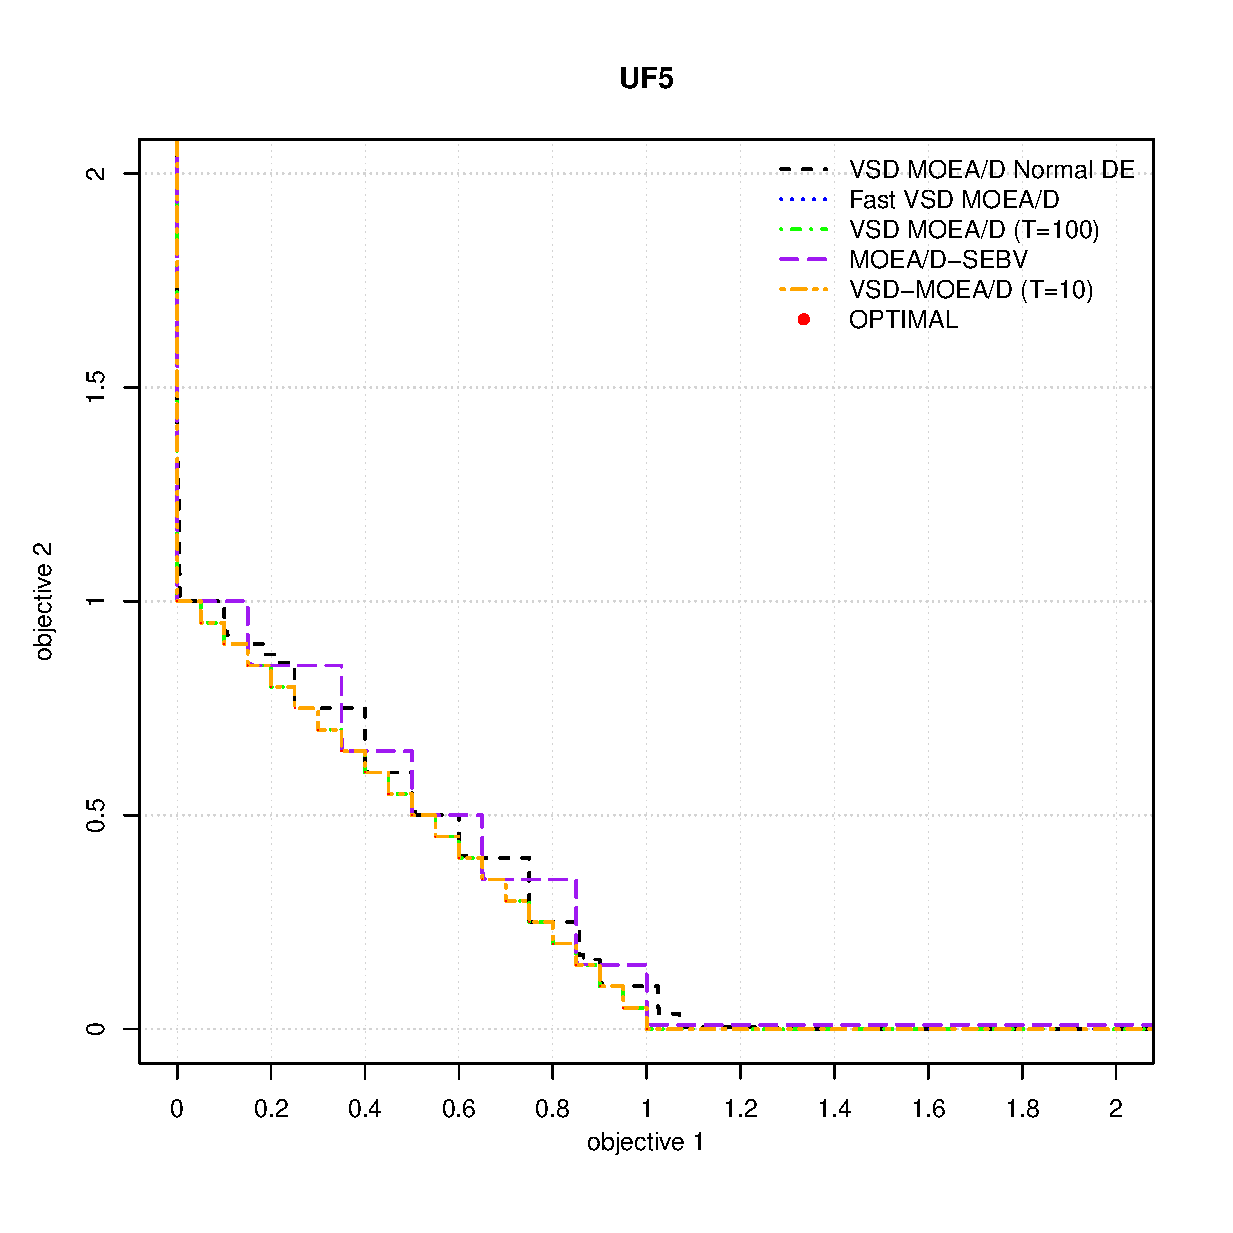
\includegraphics[width=0.33\textwidth]{Figures_Chapter7/Results_Chapter4/Surface_eps_VSD_MOEA/UF5.eps} &
  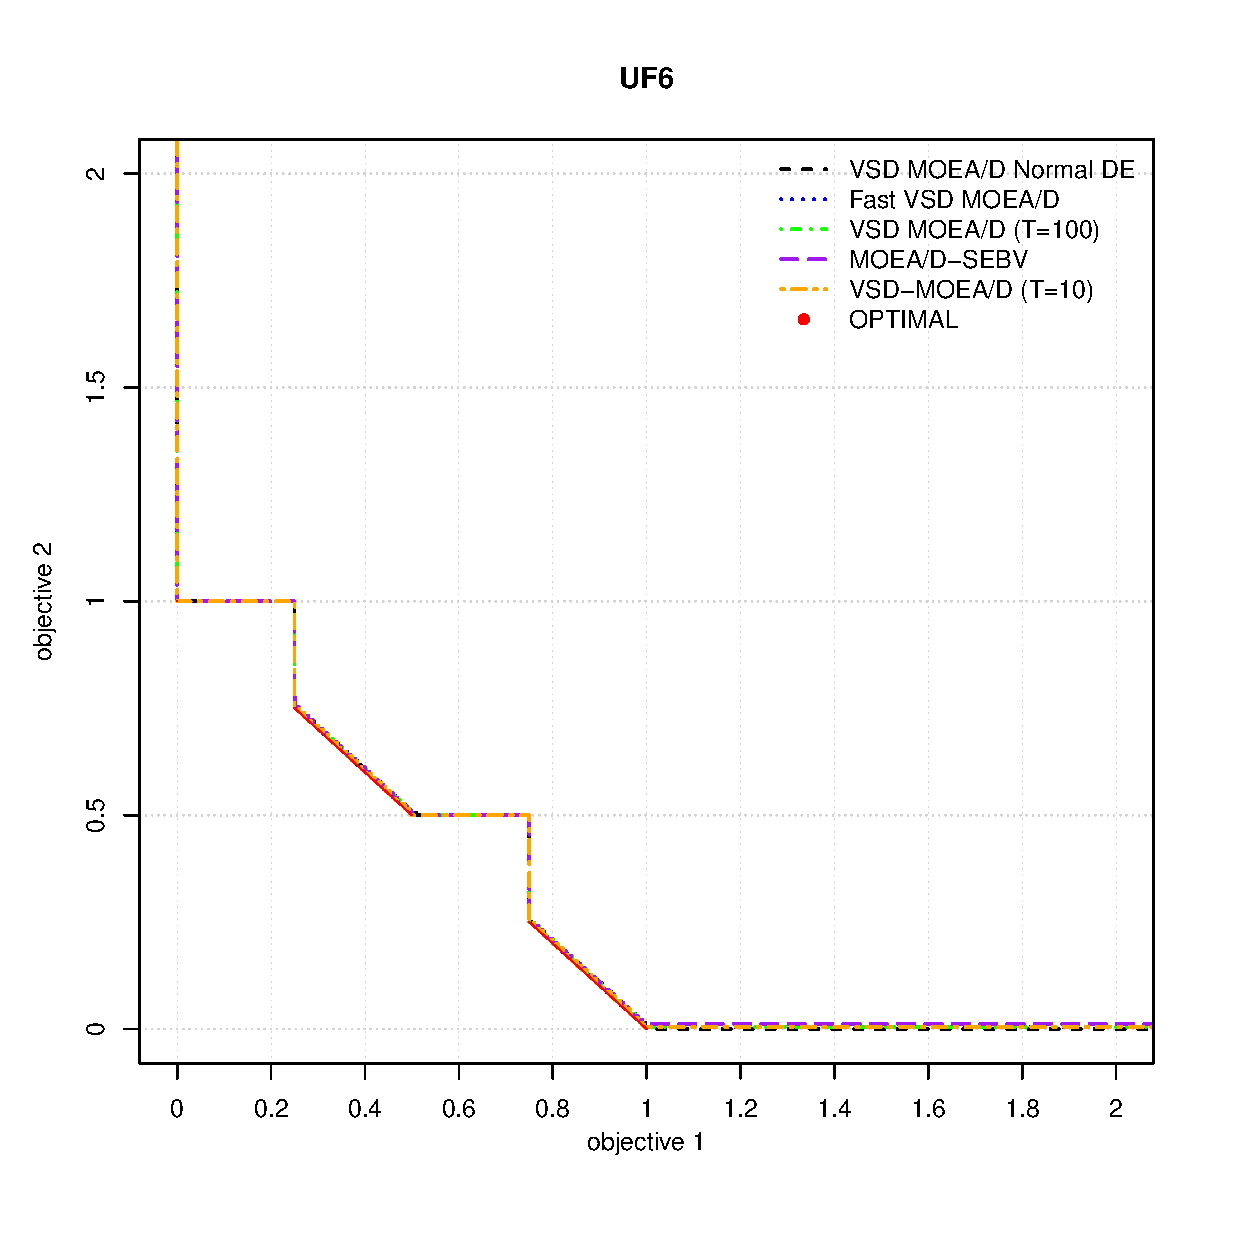
\includegraphics[width=0.33\textwidth]{Figures_Chapter7/Results_Chapter4/Surface_eps_VSD_MOEA/UF6.eps} \\
  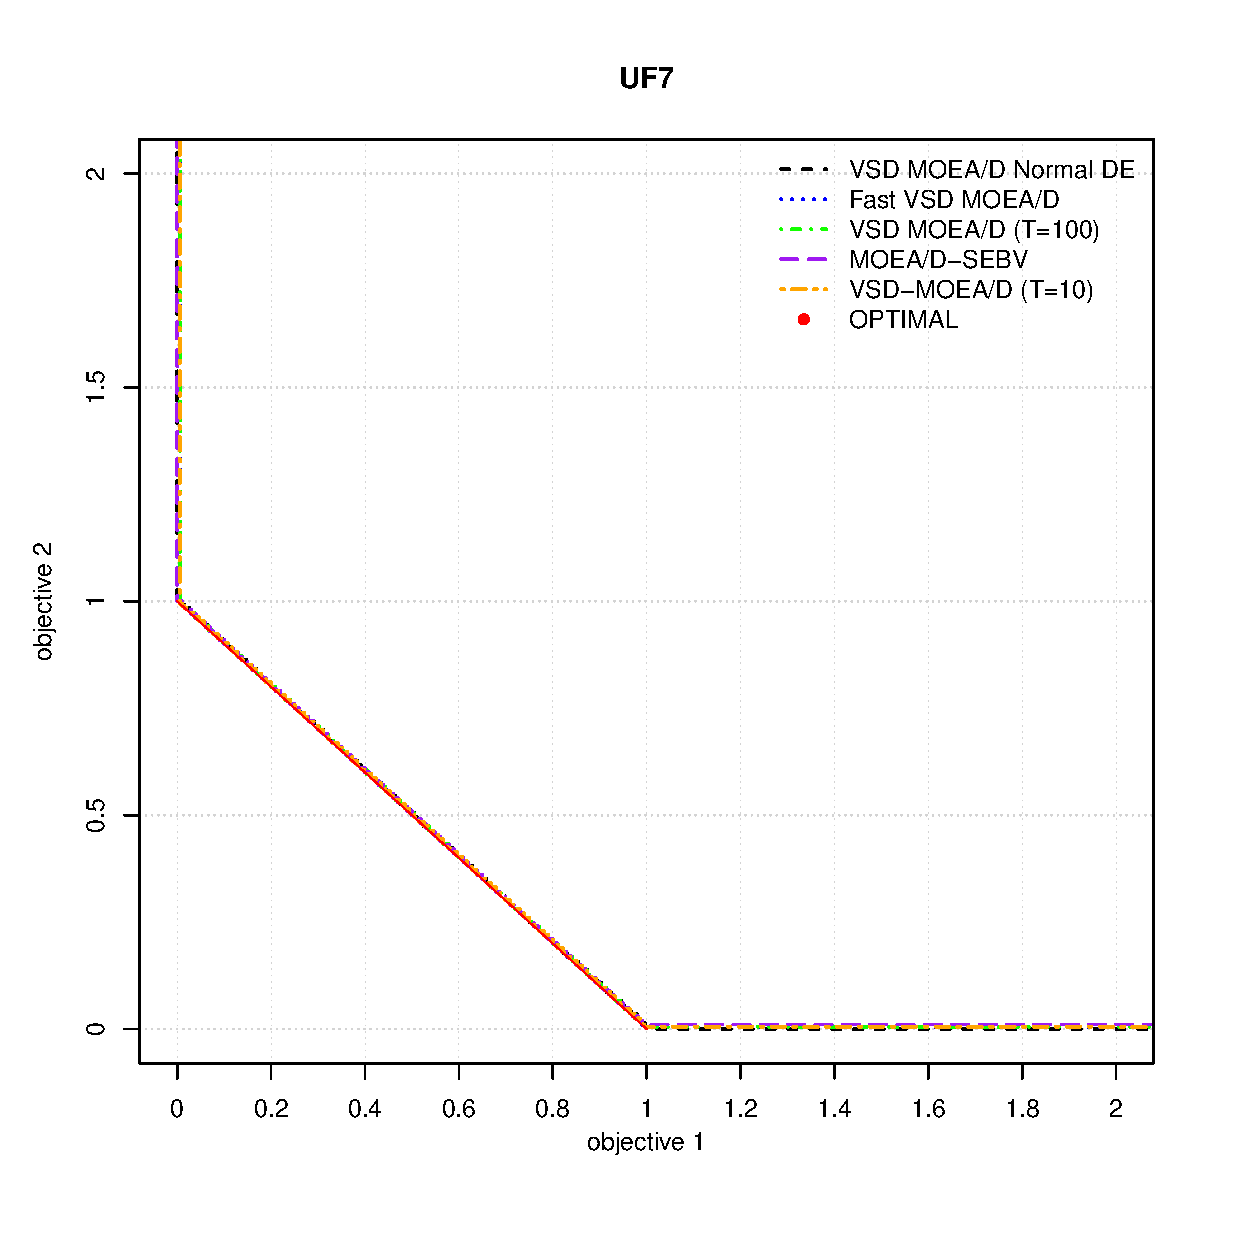
\includegraphics[width=0.33\textwidth]{Figures_Chapter7/Results_Chapter4/Surface_eps_VSD_MOEA/UF7.eps} 
\end{tabular}
\end{figure}

% Please add the following required packages to your document preamble:
% \usepackage{graphicx}
\begin{table}[]
\centering
\caption{Estadísticas del hipervolumen con dos objetivos de los algoritmos representativos}
\label{my-label}
\resizebox{\textwidth}{!}{%
\begin{tabular}{c|c|c|c|c|c|c|c|c|c|c|c|c|c|c|c|c|c|c|c|c|l|l|l|l|}
\cline{2-25}
 & \multicolumn{4}{c|}{GDE3} & \multicolumn{4}{c|}{MOMBI-II} & \multicolumn{4}{c|}{NSGAII} & \multicolumn{4}{c|}{MOEA/D} & \multicolumn{4}{c|}{VSD-MOEA} & \multicolumn{4}{c|}{VSD-MOEA/D} \\ \cline{2-25} 
 & Min & Max & Mean & Diff & Min & Max & Mean & Diff & Min & Max & Mean & Diff & Min & Max & Mean & Diff & Min & Max & Mean & Diff & Min & Max & Men & Diff \\ \hline
\multicolumn{1}{|c|}{DTLZ1} & 1.08 & 1.08 & \textbf{1.08} & 0.00 & 1.08 & 1.08 & 1.08 & 0.01 & 1.08 & 1.08 & \textbf{1.08} & 0.00 & 1.08 & 1.08 & \textbf{1.08} & 0.00 & 1.08 & 1.08 & \textbf{1.08} & 0.00 & 1.08 & 1.08 & \textbf{1.08} & 0.00 \\ \hline
\multicolumn{1}{|c|}{DTLZ2} & 0.42 & 0.42 & \textbf{0.42} & 0.00 & 0.42 & 0.42 & \textbf{0.42} & 0.00 & 0.42 & 0.42 & \textbf{0.42} & 0.00 & 0.42 & 0.42 & \textbf{0.42} & 0.00 & 0.42 & 0.42 & \textbf{0.42} & 0.00 & 0.42 & 0.42 & \textbf{0.42} & 0.00 \\ \hline
\multicolumn{1}{|c|}{DTLZ3} & 8.21 & 8.21 & \textbf{8.21} & 0.00 & 8.17 & 8.17 & 8.17 & 0.04 & 8.21 & 8.21 & \textbf{8.21} & 0.00 & 8.17 & 8.21 & 8.20 & 0.01 & 8.21 & 8.21 & \textbf{8.21} & 0.00 & 8.21 & 8.21 & \textbf{8.21} & 0.00 \\ \hline
\multicolumn{1}{|c|}{DTLZ4} & 0.42 & 0.42 & \textbf{0.42} & 0.00 & 0.11 & 0.42 & 0.38 & 0.04 & 0.11 & 0.42 & 0.31 & 0.11 & 0.11 & 0.42 & 0.37 & 0.06 & 0.42 & 0.42 & \textbf{0.42} & 0.00 & 0.42 & 0.42 & \textbf{0.42} & 0.00 \\ \hline
\multicolumn{1}{|c|}{DTLZ5} & 8.21 & 8.21 & \textbf{8.21} & 0.00 & 8.17 & 8.17 & 8.17 & 0.04 & 8.21 & 8.21 & \textbf{8.21} & 0.00 & 8.21 & 8.21 & \textbf{8.21} & 0.00 & 8.21 & 8.21 & \textbf{8.21} & 0.00 & 8.21 & 8.21 & \textbf{8.21} & 0.00 \\ \hline
\multicolumn{1}{|c|}{DTLZ6} & 8.21 & 8.21 & \textbf{8.21} & 0.00 & 7.99 & 8.17 & 8.07 & 0.14 & 8.06 & 8.21 & 8.13 & 0.08 & 8.03 & 8.21 & 8.09 & 0.12 & 7.99 & 8.21 & 8.12 & 0.09 & 8.21 & 8.21 & \textbf{8.21} & 0.00 \\ \hline
\multicolumn{1}{|c|}{DTLZ7} & 0.89 & 0.89 & \textbf{0.89} & 0.00 & 0.42 & 0.42 & 0.42 & 0.48 & 0.42 & 0.42 & 0.42 & 0.47 & 0.42 & 0.42 & 0.42 & 0.47 & 0.89 & 0.89 & \textbf{0.89} & 0.00 & 0.89 & 0.89 & \textbf{0.89} & 0.00 \\ \hline
\multicolumn{1}{|c|}{UF1} & 3.66 & 3.66 & \textbf{3.66} & 0.00 & 3.33 & 3.52 & 3.49 & 0.17 & 3.65 & 3.65 & 3.65 & 0.01 & 3.43 & 3.66 & 3.59 & 0.07 & 3.66 & 3.66 & \textbf{3.66} & 0.00 & 3.65 & 3.65 & 3.65 & 0.01 \\ \hline
\multicolumn{1}{|c|}{UF2} & 3.65 & 3.65 & \textbf{3.65} & 0.00 & 3.41 & 3.63 & 3.59 & 0.06 & 3.64 & 3.65 & 3.64 & 0.01 & 3.43 & 3.65 & 3.53 & 0.12 & 3.65 & 3.66 & \textbf{3.66} & 0.00 & 3.65 & 3.65 & 3.65 & 0.01 \\ \hline
\multicolumn{1}{|c|}{UF3} & 3.37 & 3.66 & 3.64 & 0.01 & 3.33 & 3.60 & 3.50 & 0.15 & 3.52 & 3.64 & 3.60 & 0.05 & 2.85 & 3.64 & 3.45 & 0.20 & 3.55 & 3.62 & 3.59 & 0.06 & 3.65 & 3.65 & \textbf{3.65} & 0.00 \\ \hline
\multicolumn{1}{|c|}{UF4} & 3.22 & 3.24 & 3.22 & 0.04 & 3.19 & 3.21 & 3.20 & 0.06 & 3.20 & 3.21 & 3.20 & 0.06 & 3.21 & 3.24 & 3.23 & 0.03 & 3.24 & 3.28 & \textbf{3.26} & 0.00 & 3.25 & 3.26 & 3.25 & 0.01 \\ \hline
\multicolumn{1}{|c|}{UF5} & 2.53 & 3.00 & 2.96 & 0.51 & 2.05 & 2.75 & 2.52 & 0.95 & 1.86 & 2.90 & 2.60 & 0.87 & 1.80 & 2.55 & 2.19 & 1.29 & 2.59 & 3.27 & 2.95 & 0.52 & 3.47 & 3.48 & \textbf{3.47} & 0.00 \\ \hline
\multicolumn{1}{|c|}{UF6} & 2.00 & 3.33 & 3.10 & 0.33 & 2.01 & 2.89 & 2.64 & 0.79 & 2.01 & 2.90 & 2.52 & 0.91 & 0.73 & 2.88 & 2.07 & 1.36 & 2.89 & 3.31 & 3.06 & 0.37 & 3.43 & 3.43 & \textbf{3.43} & 0.00 \\ \hline
\multicolumn{1}{|c|}{UF7} & 3.49 & 3.49 & \textbf{3.49} & 0.00 & 2.47 & 3.47 & 2.59 & 0.90 & 2.17 & 3.48 & 3.19 & 0.30 & 2.01 & 3.49 & 2.74 & 0.75 & 3.47 & 3.49 & \textbf{3.49} & 0.00 & 3.48 & 3.48 & 3.48 & 0.01 \\ \hline
\multicolumn{1}{|c|}{WFG1} & 4.26 & 5.26 & 4.85 & 0.41 & 4.62 & 5.67 & \textbf{5.26} & 0.00 & 4.72 & 5.25 & 5.16 & 0.10 & 4.48 & 5.24 & 5.04 & 0.22 & 4.72 & 5.25 & 5.20 & 0.05 & 5.05 & 5.25 & 5.22 & 0.04 \\ \hline
\multicolumn{1}{|c|}{WFG2} & 5.07 & 5.07 & \textbf{5.07} & 0.00 & 4.92 & 4.94 & 4.93 & 0.14 & 4.95 & 5.07 & 4.95 & 0.12 & 4.94 & 4.94 & 4.94 & 0.13 & 5.07 & 5.07 & \textbf{5.07} & 0.00 & 5.06 & 5.06 & 5.06 & 0.01 \\ \hline
\multicolumn{1}{|c|}{WFG3} & 4.51 & 4.53 & 4.52 & 0.04 & 4.56 & 4.56 & \textbf{4.56} & 0.00 & 4.53 & 4.54 & 4.54 & 0.03 & 4.56 & 4.56 & \textbf{4.56} & 0.00 & 4.56 & 4.57 & \textbf{4.57} & 0.00 & 4.56 & 4.56 & \textbf{4.56} & 0.00 \\ \hline
\multicolumn{1}{|c|}{WFG4} & 2.28 & 2.29 & 2.28 & 0.01 & 2.28 & 2.29 & 2.28 & 0.01 & 2.27 & 2.28 & 2.28 & 0.01 & 2.29 & 2.29 & \textbf{2.29} & 0.00 & 2.29 & 2.29 & \textbf{2.29} & 0.00 & 2.28 & 2.28 & 2.28 & 0.01 \\ \hline
\multicolumn{1}{|c|}{WFG5} & 1.98 & 1.99 & \textbf{1.99} & 0.00 & 1.98 & 2.00 & 1.98 & 0.01 & 1.97 & 1.98 & 1.97 & 0.01 & 1.97 & 2.01 & 1.98 & 0.01 & 1.98 & 1.98 & 1.98 & 0.01 & 1.97 & 2.00 & \textbf{1.98} & 0.00 \\ \hline
\multicolumn{1}{|c|}{WFG6} & 2.09 & 2.25 & 2.18 & 0.10 & 2.05 & 2.21 & 2.14 & 0.14 & 2.06 & 2.21 & 2.14 & 0.14 & 2.02 & 2.19 & 2.13 & 0.15 & 2.08 & 2.20 & 2.13 & 0.15 & 2.26 & 2.28 & \textbf{2.28} & 0.00 \\ \hline
\multicolumn{1}{|c|}{WFG7} & 2.27 & 2.28 & 2.28 & 0.02 & 2.28 & 2.28 & 2.28 & 0.01 & 2.27 & 2.28 & 2.28 & 0.02 & 2.29 & 2.29 & \textbf{2.29} & 0.00 & 2.29 & 2.29 & \textbf{2.29} & 0.00 & 2.28 & 2.28 & 2.28 & 0.01 \\ \hline
\multicolumn{1}{|c|}{WFG8} & 1.86 & 1.88 & 1.87 & 0.37 & 1.87 & 2.24 & 1.95 & 0.29 & 1.80 & 2.14 & 1.91 & 0.33 & 1.94 & 2.25 & 2.23 & 0.01 & 2.05 & 2.25 & 2.23 & 0.01 & 2.11 & 2.27 & \textbf{2.24} & 0.00 \\ \hline
\multicolumn{1}{|c|}{WFG9} & 1.71 & 1.71 & 1.71 & 0.54 & 2.20 & 2.26 & 2.24 & 0.01 & 2.17 & 2.26 & 2.23 & 0.03 & 1.71 & 2.26 & 2.22 & 0.03 & 2.24 & 2.27 & \textbf{2.25} & 0.00 & 2.25 & 2.26 & \textbf{2.25} & 0.00 \\ \hline
\multicolumn{1}{|c|}{Average} & 3.279 & 3.423 & 3.388 & \textbf{0.103} & 3.170 & 3.406 & 3.299 & \textbf{0.193} & 3.187 & 3.409 & 3.332 & \textbf{0.160} & 3.047 & 3.397 & 3.272 & \textbf{0.219} & 3.372 & 3.474 & 3.437 & \textbf{0.055} & 3.471 & 3.491 & 3.487 & \textbf{0.005} \\ \hline
\end{tabular}%
}
\end{table}



% Please add the following required packages to your document preamble:
% \usepackage{graphicx}
\begin{table}[]
\centering
\caption{Estadísticas del IGD+ con dos objetivos de los algoritmos representativos}
\label{my-label}
\resizebox{\textwidth}{!}{%
\begin{tabular}{c|c|c|c|c|c|c|c|c|c|c|c|c|c|c|c|c|c|c|c|c|l|l|l|l|}
\cline{2-25}
 & \multicolumn{4}{c|}{GDE3} & \multicolumn{4}{c|}{MOMBI-II} & \multicolumn{4}{c|}{NSGAII} & \multicolumn{4}{c|}{MOEA/D} & \multicolumn{4}{c|}{VSD-MOEA} & \multicolumn{4}{c|}{VSD-MOEA/D} \\ \cline{2-25} 
 & Min & Max & Mean & Diff & Min & Max & Mean & Diff & Min & Max & Mean & Diff & Min & Max & Mean & Diff & Min & Max & Mean & Diff & Min & Max & Men & Diff \\ \hline
\multicolumn{1}{|c|}{DTLZ1} & 0.001 & 0.001 & \textbf{0.001} & 0.000 & 0.001 & 0.001 & \textbf{0.001} & 0.000 & 0.002 & 0.002 & \textbf{0.002} & 0.000 & 0.001 & 0.001 & \textbf{0.001} & 0.000 & 0.001 & 0.001 & \textbf{0.001} & 0.000 & 0.001 & 0.001 & \textbf{0.001} & 0.000 \\ \hline
\multicolumn{1}{|c|}{DTLZ2} & 0.002 & 0.002 & \textbf{0.002} & 0.000 & 0.002 & 0.002 & \textbf{0.002} & 0.000 & 0.002 & 0.003 & 0.003 & 0.001 & 0.002 & 0.002 & \textbf{0.002} & 0.000 & 0.002 & 0.002 & \textbf{0.002} & 0.000 & 0.002 & 0.002 & \textbf{0.002} & 0.000 \\ \hline
\multicolumn{1}{|c|}{DTLZ3} & 0.002 & 0.002 & \textbf{0.002} & 0.000 & 0.002 & 0.002 & \textbf{0.002} & 0.000 & 0.002 & 0.003 & 0.003 & 0.001 & 0.002 & 0.002 & \textbf{0.002} & 0.000 & 0.002 & 0.002 & \textbf{0.002} & 0.000 & 0.002 & 0.002 & \textbf{0.002} & 0.000 \\ \hline
\multicolumn{1}{|c|}{DTLZ4} & 0.002 & 0.002 & \textbf{0.002} & 0.000 & 0.002 & 0.363 & 0.043 & 0.042 & 0.002 & 0.363 & 0.126 & 0.124 & 0.002 & 0.363 & 0.064 & 0.062 & 0.002 & 0.002 & \textbf{0.002} & 0.000 & 0.002 & 0.002 & \textbf{0.002} & 0.000 \\ \hline
\multicolumn{1}{|c|}{DTLZ5} & 0.002 & 0.002 & \textbf{0.002} & 0.000 & 0.002 & 0.002 & \textbf{0.002} & 0.000 & 0.002 & 0.003 & 0.003 & 0.001 & 0.002 & 0.002 & \textbf{0.002} & 0.000 & 0.002 & 0.002 & \textbf{0.002} & 0.000 & 0.002 & 0.002 & \textbf{0.002} & 0.000 \\ \hline
\multicolumn{1}{|c|}{DTLZ6} & 0.002 & 0.002 & \textbf{0.002} & 0.000 & 0.002 & 0.108 & 0.059 & 0.057 & 0.003 & 0.089 & 0.051 & 0.049 & 0.002 & 0.110 & 0.067 & 0.065 & 0.002 & 0.132 & 0.054 & 0.052 & 0.002 & 0.002 & \textbf{0.002} & 0.000 \\ \hline
\multicolumn{1}{|c|}{DTLZ7} & 0.002 & 0.002 & \textbf{0.002} & 0.000 & 0.363 & 0.363 & 0.363 & 0.361 & 0.361 & 0.361 & 0.361 & 0.359 & 0.361 & 0.361 & 0.361 & 0.359 & 0.003 & 0.003 & 0.003 & 0.001 & 0.003 & 0.003 & 0.003 & 0.001 \\ \hline
\multicolumn{1}{|c|}{UF1} & 0.004 & 0.005 & 0.004 & 0.002 & 0.008 & 0.037 & 0.011 & 0.009 & 0.008 & 0.009 & 0.009 & 0.006 & 0.003 & 0.034 & 0.011 & 0.009 & 0.002 & 0.007 & 0.003 & 0.001 & 0.003 & 0.003 & \textbf{0.003} & 0.000 \\ \hline
\multicolumn{1}{|c|}{UF2} & 0.007 & 0.009 & 0.008 & 0.005 & 0.004 & 0.042 & 0.008 & 0.005 & 0.011 & 0.014 & 0.013 & 0.010 & 0.003 & 0.041 & 0.019 & 0.016 & 0.004 & 0.007 & 0.005 & 0.003 & 0.003 & 0.003 & \textbf{0.003} & 0.000 \\ \hline
\multicolumn{1}{|c|}{UF3} & 0.003 & 0.168 & 0.013 & 0.011 & 0.017 & 0.046 & 0.030 & 0.027 & 0.015 & 0.034 & 0.024 & 0.021 & 0.007 & 0.196 & 0.037 & 0.035 & 0.028 & 0.058 & 0.040 & 0.038 & 0.002 & 0.002 & \textbf{0.002} & 0.000 \\ \hline
\multicolumn{1}{|c|}{UF4} & 0.035 & 0.038 & 0.037 & 0.013 & 0.037 & 0.041 & 0.040 & 0.016 & 0.043 & 0.047 & 0.046 & 0.022 & 0.032 & 0.041 & 0.036 & 0.012 & 0.023 & 0.035 & 0.027 & 0.003 & 0.023 & 0.026 & \textbf{0.024} & 0.000 \\ \hline
\multicolumn{1}{|c|}{UF5} & 0.238 & 0.275 & 0.245 & 0.245 & 0.174 & 0.481 & 0.300 & 0.300 & 0.146 & 0.570 & 0.287 & 0.286 & 0.229 & 0.571 & 0.385 & 0.385 & 0.113 & 0.371 & 0.197 & 0.196 & 0.000 & 0.005 & \textbf{0.000} & 0.000 \\ \hline
\multicolumn{1}{|c|}{UF6} & 0.029 & 0.417 & 0.125 & 0.123 & 0.169 & 0.570 & 0.292 & 0.290 & 0.167 & 0.577 & 0.341 & 0.339 & 0.173 & 1.076 & 0.529 & 0.527 & 0.044 & 0.171 & 0.121 & 0.119 & 0.002 & 0.002 & \textbf{0.002} & 0.000 \\ \hline
\multicolumn{1}{|c|}{UF7} & 0.004 & 0.005 & 0.004 & 0.002 & 0.004 & 0.254 & 0.230 & 0.227 & 0.008 & 0.385 & 0.083 & 0.081 & 0.003 & 0.492 & 0.194 & 0.191 & 0.004 & 0.013 & 0.005 & 0.003 & 0.003 & 0.003 & \textbf{0.003} & 0.000 \\ \hline
\multicolumn{1}{|c|}{WFG1} & 0.005 & 0.214 & 0.088 & 0.075 & 0.000 & 0.137 & 0.029 & 0.016 & 0.006 & 0.113 & 0.024 & 0.011 & 0.008 & 0.166 & 0.049 & 0.036 & 0.006 & 0.115 & 0.015 & 0.002 & 0.007 & 0.046 & \textbf{0.013} & 0.000 \\ \hline
\multicolumn{1}{|c|}{WFG2} & 0.002 & 0.002 & \textbf{0.002} & 0.000 & 0.055 & 0.057 & 0.057 & 0.055 & 0.003 & 0.054 & 0.052 & 0.049 & 0.055 & 0.055 & 0.055 & 0.053 & 0.003 & 0.003 & 0.003 & 0.001 & 0.006 & 0.006 & 0.006 & 0.004 \\ \hline
\multicolumn{1}{|c|}{WFG3} & 0.014 & 0.017 & 0.015 & 0.008 & 0.007 & 0.007 & \textbf{0.007} & 0.000 & 0.011 & 0.013 & 0.012 & 0.005 & 0.008 & 0.008 & 0.008 & 0.001 & 0.007 & 0.008 & \textbf{0.007} & 0.000 & 0.008 & 0.008 & 0.008 & 0.001 \\ \hline
\multicolumn{1}{|c|}{WFG4} & 0.007 & 0.008 & 0.007 & 0.001 & 0.006 & 0.006 & \textbf{0.006} & 0.000 & 0.007 & 0.009 & 0.008 & 0.002 & 0.007 & 0.007 & 0.007 & 0.001 & 0.006 & 0.006 & \textbf{0.006} & 0.000 & 0.007 & 0.007 & 0.007 & 0.001 \\ \hline
\multicolumn{1}{|c|}{WFG5} & 0.064 & 0.066 & \textbf{0.065} & 0.000 & 0.062 & 0.068 & \textbf{0.065} & 0.000 & 0.065 & 0.066 & 0.066 & 0.001 & 0.058 & 0.069 & 0.067 & 0.002 & 0.065 & 0.069 & 0.066 & 0.001 & 0.061 & 0.070 & 0.066 & 0.001 \\ \hline
\multicolumn{1}{|c|}{WFG6} & 0.014 & 0.043 & 0.025 & 0.018 & 0.020 & 0.050 & 0.032 & 0.025 & 0.021 & 0.049 & 0.034 & 0.026 & 0.024 & 0.073 & 0.037 & 0.030 & 0.022 & 0.045 & 0.035 & 0.028 & 0.007 & 0.012 & \textbf{0.007} & 0.000 \\ \hline
\multicolumn{1}{|c|}{WFG7} & 0.008 & 0.009 & 0.008 & 0.002 & 0.006 & 0.006 & \textbf{0.006} & 0.000 & 0.007 & 0.009 & 0.008 & 0.003 & 0.007 & 0.007 & 0.007 & 0.001 & 0.006 & 0.006 & \textbf{0.006} & 0.000 & 0.007 & 0.007 & 0.007 & 0.001 \\ \hline
\multicolumn{1}{|c|}{WFG8} & 0.094 & 0.098 & 0.096 & 0.078 & 0.017 & 0.092 & 0.075 & 0.057 & 0.034 & 0.103 & 0.078 & 0.060 & 0.015 & 0.068 & 0.021 & 0.003 & 0.016 & 0.050 & 0.020 & 0.002 & 0.011 & 0.039 & \textbf{0.018} & 0.000 \\ \hline
\multicolumn{1}{|c|}{WFG9} & 0.122 & 0.125 & 0.123 & 0.112 & 0.009 & 0.023 & 0.013 & 0.002 & 0.011 & 0.027 & 0.016 & 0.005 & 0.010 & 0.125 & 0.017 & 0.006 & 0.008 & 0.013 & \textbf{0.011} & 0.000 & 0.010 & 0.012 & \textbf{0.012} & 0.000 \\ \hline
\multicolumn{1}{|c|}{Average} & 0.029 & 0.066 & 0.038 & \textbf{0.030} & 0.042 & 0.120 & 0.073 & \textbf{0.065} & 0.041 & 0.126 & 0.072 & \textbf{0.064} & 0.044 & 0.168 & 0.086 & \textbf{0.078} & 0.016 & 0.049 & 0.028 & \textbf{0.020} & 0.008 & 0.012 & 0.008 & \textbf{0.000} \\ \hline
\end{tabular}%
}
\end{table}

% Please add the following required packages to your document preamble:
% \usepackage{graphicx}
\begin{table}[]
\centering
\caption{Estadísticas del hipervolumen con tres objetivos de los algoritmos representativos}
\label{my-label}
\resizebox{\textwidth}{!}{%
\begin{tabular}{c|c|c|c|c|c|c|c|c|c|c|c|c|c|c|c|c|c|c|c|c|l|l|l|l|}
\cline{2-25}
 & \multicolumn{4}{c|}{GDE3} & \multicolumn{4}{c|}{MOMBI-II} & \multicolumn{4}{c|}{NSGAII} & \multicolumn{4}{c|}{MOEA/D} & \multicolumn{4}{c|}{VSD-MOEA} & \multicolumn{4}{c|}{VSD-MOEA/D} \\ \cline{2-25} 
 & Min & Max & Mean & Diff & Min & Max & Mean & Diff & Min & Max & Mean & Diff & Min & Max & Mean & Diff & Min & Max & Mean & Diff & Min & Max & Men & Diff \\ \hline
\multicolumn{1}{|c|}{DTLZ1} & 1.30 & 1.30 & \textbf{1.30} & 0.00 & 1.29 & 1.29 & 1.29 & 0.01 & 1.30 & 1.30 & \textbf{1.30} & 0.00 & 1.28 & 1.29 & 1.29 & 0.01 & 1.30 & 1.30 & \textbf{1.30} & 0.00 & 1.29 & 1.29 & 1.29 & 0.01 \\ \hline
\multicolumn{1}{|c|}{DTLZ2} & 0.71 & 0.72 & 0.71 & 0.03 & 0.72 & 0.72 & 0.72 & 0.02 & 0.69 & 0.72 & 0.71 & 0.04 & 0.71 & 0.71 & 0.71 & 0.03 & 0.74 & 0.75 & \textbf{0.74} & 0.00 & 0.73 & 0.73 & 0.73 & 0.01 \\ \hline
\multicolumn{1}{|c|}{DTLZ3} & 26.37 & 26.39 & 26.38 & 0.03 & 26.15 & 26.15 & 26.15 & 0.26 & 26.36 & 26.39 & 26.38 & 0.04 & 26.17 & 26.27 & 26.27 & 0.15 & 26.41 & 26.41 & \textbf{26.41} & 0.00 & 26.40 & 26.40 & 26.40 & 0.01 \\ \hline
\multicolumn{1}{|c|}{DTLZ4} & 0.71 & 0.72 & 0.71 & 0.03 & 0.45 & 0.72 & 0.70 & 0.04 & 0.12 & 0.73 & 0.70 & 0.05 & 0.12 & 0.71 & 0.60 & 0.14 & 0.74 & 0.74 & \textbf{0.74} & 0.00 & 0.73 & 0.74 & 0.74 & 0.01 \\ \hline
\multicolumn{1}{|c|}{DTLZ5} & 23.99 & 23.99 & \textbf{23.99} & 0.00 & 23.81 & 23.82 & 23.81 & 0.17 & 23.98 & 23.98 & 23.98 & 0.01 & 23.88 & 23.88 & 23.88 & 0.11 & 23.99 & 23.99 & \textbf{23.99} & 0.00 & 23.90 & 23.90 & 23.90 & 0.09 \\ \hline
\multicolumn{1}{|c|}{DTLZ6} & 23.99 & 23.99 & \textbf{23.99} & 0.00 & 23.36 & 23.81 & 23.58 & 0.41 & 23.70 & 23.98 & 23.82 & 0.17 & 23.27 & 23.71 & 23.53 & 0.45 & 23.48 & 23.99 & 23.74 & 0.25 & 23.90 & 23.90 & 23.90 & 0.09 \\ \hline
\multicolumn{1}{|c|}{DTLZ7} & 1.78 & 1.84 & 1.82 & 0.05 & 0.90 & 0.90 & 0.90 & 0.97 & 0.89 & 0.91 & 0.90 & 0.97 & 0.90 & 0.91 & 0.90 & 0.96 & 1.86 & 1.88 & \textbf{1.87} & 0.00 & 1.76 & 1.76 & 1.76 & 0.11 \\ \hline
\multicolumn{1}{|c|}{UF10} & 0.01 & 3.89 & 0.66 & 6.65 & 3.15 & 5.58 & 3.96 & 3.35 & 3.76 & 6.26 & 4.66 & 2.65 & 2.91 & 4.08 & 3.55 & 3.76 & 6.00 & 7.24 & 6.89 & 0.42 & 7.27 & 7.36 & \textbf{7.31} & 0.00 \\ \hline
\multicolumn{1}{|c|}{UF8} & 0.05 & 4.85 & 1.97 & 5.43 & 4.00 & 7.36 & 6.91 & 0.50 & 7.16 & 7.27 & 7.23 & 0.18 & 4.00 & 7.32 & 6.41 & 0.99 & 7.32 & 7.41 & 7.39 & 0.02 & 7.40 & 7.41 & \textbf{7.41} & 0.00 \\ \hline
\multicolumn{1}{|c|}{UF9} & 0.24 & 4.22 & 1.49 & 6.26 & 7.13 & 7.65 & 7.26 & 0.49 & 6.89 & 7.60 & 7.35 & 0.40 & 7.11 & 7.65 & 7.23 & 0.52 & 7.72 & 7.76 & \textbf{7.75} & 0.00 & 7.68 & 7.71 & 7.70 & 0.05 \\ \hline
\multicolumn{1}{|c|}{WFG1} & 16.34 & 18.10 & 17.10 & 28.88 & 40.29 & 48.67 & \textbf{45.98} & 0.00 & 43.05 & 44.55 & 43.64 & 2.34 & 40.35 & 44.99 & 43.65 & 2.34 & 45.44 & 45.94 & 45.76 & 0.22 & 44.82 & 45.40 & 45.25 & 0.73 \\ \hline
\multicolumn{1}{|c|}{WFG2} & 45.96 & 47.22 & 46.71 & 1.82 & 40.20 & 48.21 & 45.18 & 3.35 & 40.09 & 47.47 & 45.54 & 2.99 & 40.04 & 47.80 & 43.55 & 4.98 & 48.35 & 48.67 & \textbf{48.53} & 0.00 & 47.83 & 47.83 & 47.83 & 0.70 \\ \hline
\multicolumn{1}{|c|}{WFG3} & 30.39 & 31.00 & 30.73 & 0.48 & 31.16 & 31.19 & 31.18 & 0.03 & 30.59 & 31.14 & 30.90 & 0.30 & 31.15 & 31.16 & 31.15 & 0.05 & 31.03 & 31.07 & 31.05 & 0.16 & 31.20 & 31.21 & \textbf{31.21} & 0.00 \\ \hline
\multicolumn{1}{|c|}{WFG4} & 18.01 & 20.15 & 19.18 & 4.96 & 23.63 & 23.66 & 23.64 & 0.50 & 21.72 & 22.75 & 22.30 & 1.84 & 21.93 & 22.47 & 22.13 & 2.01 & 23.98 & 24.32 & \textbf{24.13} & 0.00 & 23.19 & 23.35 & 23.26 & 0.88 \\ \hline
\multicolumn{1}{|c|}{WFG5} & 20.14 & 21.17 & 20.68 & 1.21 & 21.39 & 21.40 & 21.40 & 0.50 & 19.99 & 21.05 & 20.59 & 1.30 & 19.68 & 20.36 & 19.76 & 2.13 & 21.73 & 22.08 & \textbf{21.89} & 0.00 & 20.62 & 21.08 & 20.76 & 1.13 \\ \hline
\multicolumn{1}{|c|}{WFG6} & 17.31 & 20.48 & 18.93 & 4.12 & 22.01 & 23.02 & 22.65 & 0.39 & 19.84 & 22.02 & 21.02 & 2.02 & 20.34 & 21.58 & 21.04 & 2.00 & 22.50 & 23.42 & \textbf{23.04} & 0.00 & 22.17 & 23.23 & 23.02 & 0.02 \\ \hline
\multicolumn{1}{|c|}{WFG7} & 18.96 & 20.97 & 19.86 & 4.27 & 23.63 & 23.65 & 23.64 & 0.49 & 21.55 & 22.97 & 22.44 & 1.69 & 22.26 & 22.26 & 22.26 & 1.87 & 23.91 & 24.34 & \textbf{24.13} & 0.00 & 23.18 & 23.28 & 23.22 & 0.91 \\ \hline
\multicolumn{1}{|c|}{WFG8} & 14.14 & 15.49 & 14.73 & 8.42 & 20.80 & 23.72 & 23.13 & 0.02 & 16.29 & 18.40 & 17.76 & 5.39 & 21.69 & 22.10 & 21.86 & 1.30 & 18.99 & 24.08 & \textbf{23.15} & 0.00 & 20.06 & 23.42 & 22.89 & 0.27 \\ \hline
\multicolumn{1}{|c|}{WFG9} & 17.52 & 18.36 & 18.00 & 5.07 & 19.11 & 23.27 & 22.85 & 0.22 & 17.28 & 21.26 & 18.06 & 5.01 & 17.68 & 21.80 & 21.24 & 1.83 & 19.26 & 23.79 & \textbf{23.07} & 0.00 & 21.92 & 22.63 & 22.31 & 0.76 \\ \hline
\multicolumn{1}{|c|}{Average} & 14.627 & 16.045 & 15.207 & \textbf{4.091} & 17.537 & 19.202 & 18.680 & \textbf{0.617} & 17.118 & 18.460 & 17.857 & \textbf{1.440} & 17.130 & 18.476 & 17.949 & \textbf{1.348} & 18.671 & 19.430 & 19.241 & \textbf{0.056} & 18.739 & 19.086 & 18.993 & \textbf{0.304} \\ \hline
\end{tabular}%
}
\end{table}


% Please add the following required packages to your document preamble:
% \usepackage{graphicx}
\begin{table}[]
\caption{Estadísticas del IGD+ con tres objetivos de los algoritmos representativos}
\label{my-label}
\resizebox{\textwidth}{!}{%
\begin{tabular}{c|c|c|c|c|c|c|c|c|c|c|c|c|c|c|c|c|c|c|c|c|l|l|l|l|}
\cline{2-25}
 & \multicolumn{4}{c|}{GDE3} & \multicolumn{4}{c|}{MOMBI-II} & \multicolumn{4}{c|}{NSGA-II} & \multicolumn{4}{c|}{MOEA/D} & \multicolumn{4}{c|}{VSD-MOEA} & \multicolumn{4}{c|}{VSD-MOEA/D} \\ \cline{2-25} 
 & Min & Max & Mean & Diff & Min & Max & Mean & Diff & Min & Max & Mean & Diff & Min & Max & Mean & Diff & Min & Max & Mean & Diff & Min & Max & Men & Diff \\ \hline
\multicolumn{1}{|c|}{DTLZ1} & 0.017 & 0.021 & 0.019 & 0.006 & 0.013 & 0.013 & \textbf{0.013} & 0.000 & 0.018 & 0.023 & 0.020 & 0.007 & 0.014 & 0.014 & 0.014 & 0.001 & 0.013 & 0.015 & 0.014 & 0.001 & 0.013 & 0.013 & \textbf{0.013} & 0.000 \\ \hline
\multicolumn{1}{|c|}{DTLZ2} & 0.027 & 0.032 & 0.030 & 0.007 & 0.025 & 0.025 & 0.025 & 0.001 & 0.028 & 0.036 & 0.032 & 0.008 & 0.028 & 0.028 & 0.028 & 0.004 & 0.023 & 0.025 & \textbf{0.024} & 0.000 & 0.024 & 0.024 & \textbf{0.024} & 0.000 \\ \hline
\multicolumn{1}{|c|}{DTLZ3} & 0.028 & 0.035 & 0.031 & 0.007 & 0.025 & 0.025 & 0.025 & 0.001 & 0.028 & 0.037 & 0.031 & 0.008 & 0.028 & 0.028 & 0.028 & 0.004 & 0.024 & 0.024 & \textbf{0.024} & 0.000 & 0.024 & 0.024 & \textbf{0.024} & 0.000 \\ \hline
\multicolumn{1}{|c|}{DTLZ4} & 0.028 & 0.033 & 0.030 & 0.006 & 0.025 & 0.364 & 0.042 & 0.018 & 0.028 & 0.595 & 0.046 & 0.022 & 0.028 & 0.595 & 0.107 & 0.083 & 0.024 & 0.024 & 0.024 & 0.001 & 0.024 & 0.024 & \textbf{0.024} & 0.000 \\ \hline
\multicolumn{1}{|c|}{DTLZ5} & 0.002 & 0.002 & \textbf{0.002} & 0.000 & 0.004 & 0.004 & 0.004 & 0.002 & 0.003 & 0.003 & 0.003 & 0.001 & 0.003 & 0.003 & 0.003 & 0.001 & 0.002 & 0.002 & \textbf{0.002} & 0.000 & 0.003 & 0.003 & 0.003 & 0.001 \\ \hline
\multicolumn{1}{|c|}{DTLZ6} & 0.002 & 0.002 & \textbf{0.002} & 0.000 & 0.004 & 0.125 & 0.065 & 0.064 & 0.003 & 0.072 & 0.041 & 0.039 & 0.045 & 0.159 & 0.094 & 0.092 & 0.002 & 0.124 & 0.060 & 0.058 & 0.003 & 0.003 & 0.003 & 0.001 \\ \hline
\multicolumn{1}{|c|}{DTLZ7} & 0.031 & 0.043 & 0.035 & 0.007 & 0.688 & 0.689 & 0.689 & 0.661 & 0.683 & 0.684 & 0.683 & 0.655 & 0.685 & 0.685 & 0.685 & 0.657 & 0.027 & 0.029 & \textbf{0.028} & 0.000 & 0.047 & 0.047 & 0.047 & 0.019 \\ \hline
\multicolumn{1}{|c|}{UF10} & 0.609 & 2.740 & 1.545 & 1.486 & 0.182 & 0.473 & 0.339 & 0.280 & 0.178 & 0.388 & 0.308 & 0.250 & 0.326 & 0.478 & 0.389 & 0.330 & 0.075 & 0.225 & 0.101 & 0.043 & 0.044 & 0.061 & \textbf{0.059} & 0.000 \\ \hline
\multicolumn{1}{|c|}{UF8} & 0.442 & 2.747 & 1.259 & 1.235 & 0.035 & 0.365 & 0.098 & 0.074 & 0.071 & 0.089 & 0.078 & 0.054 & 0.035 & 0.365 & 0.137 & 0.113 & 0.025 & 0.060 & 0.034 & 0.010 & 0.024 & 0.025 & \textbf{0.024} & 0.000 \\ \hline
\multicolumn{1}{|c|}{UF9} & 0.701 & 2.225 & 1.345 & 1.320 & 0.025 & 0.143 & 0.113 & 0.087 & 0.073 & 0.229 & 0.128 & 0.102 & 0.034 & 0.143 & 0.124 & 0.099 & 0.023 & 0.033 & 0.027 & 0.001 & 0.025 & 0.026 & \textbf{0.025} & 0.000 \\ \hline
\multicolumn{1}{|c|}{WFG1} & 1.169 & 1.276 & 1.236 & 1.172 & 0.008 & 0.224 & \textbf{0.064} & 0.000 & 0.123 & 0.168 & 0.141 & 0.077 & 0.080 & 0.209 & 0.122 & 0.058 & 0.052 & 0.099 & \textbf{0.064} & 0.000 & 0.071 & 0.140 & 0.079 & 0.015 \\ \hline
\multicolumn{1}{|c|}{WFG2} & 0.092 & 0.149 & 0.118 & 0.078 & 0.040 & 0.108 & 0.066 & 0.027 & 0.095 & 0.168 & 0.140 & 0.101 & 0.044 & 0.117 & 0.087 & 0.047 & 0.031 & 0.055 & \textbf{0.040} & 0.000 & 0.056 & 0.056 & 0.056 & 0.016 \\ \hline
\multicolumn{1}{|c|}{WFG3} & 0.046 & 0.094 & 0.066 & 0.042 & 0.024 & 0.027 & 0.026 & 0.003 & 0.032 & 0.074 & 0.047 & 0.024 & 0.024 & 0.025 & 0.025 & 0.001 & 0.036 & 0.039 & 0.037 & 0.013 & 0.023 & 0.023 & \textbf{0.023} & 0.000 \\ \hline
\multicolumn{1}{|c|}{WFG4} & 0.192 & 0.245 & 0.214 & 0.128 & 0.085 & 0.085 & \textbf{0.085} & 0.000 & 0.113 & 0.135 & 0.123 & 0.037 & 0.122 & 0.126 & 0.124 & 0.039 & 0.084 & 0.093 & 0.089 & 0.003 & 0.109 & 0.111 & 0.110 & 0.024 \\ \hline
\multicolumn{1}{|c|}{WFG5} & 0.151 & 0.171 & 0.159 & 0.014 & 0.144 & 0.145 & \textbf{0.145} & 0.000 & 0.160 & 0.177 & 0.167 & 0.022 & 0.176 & 0.185 & 0.180 & 0.035 & 0.141 & 0.152 & 0.147 & 0.002 & 0.166 & 0.171 & 0.168 & 0.024 \\ \hline
\multicolumn{1}{|c|}{WFG6} & 0.182 & 0.263 & 0.220 & 0.109 & 0.101 & 0.128 & \textbf{0.110} & 0.000 & 0.134 & 0.191 & 0.155 & 0.044 & 0.143 & 0.176 & 0.154 & 0.044 & 0.103 & 0.130 & 0.114 & 0.004 & 0.110 & 0.141 & 0.117 & 0.007 \\ \hline
\multicolumn{1}{|c|}{WFG7} & 0.174 & 0.218 & 0.197 & 0.112 & 0.085 & 0.085 & \textbf{0.085} & 0.000 & 0.107 & 0.134 & 0.120 & 0.035 & 0.126 & 0.126 & 0.126 & 0.041 & 0.084 & 0.094 & 0.089 & 0.003 & 0.110 & 0.110 & 0.110 & 0.025 \\ \hline
\multicolumn{1}{|c|}{WFG8} & 0.310 & 0.352 & 0.331 & 0.227 & 0.092 & 0.147 & \textbf{0.104} & 0.000 & 0.216 & 0.265 & 0.232 & 0.129 & 0.132 & 0.143 & 0.136 & 0.032 & 0.091 & 0.226 & 0.114 & 0.010 & 0.110 & 0.173 & 0.120 & 0.016 \\ \hline
\multicolumn{1}{|c|}{WFG9} & 0.223 & 0.247 & 0.235 & 0.135 & 0.090 & 0.208 & \textbf{0.100} & 0.000 & 0.131 & 0.250 & 0.229 & 0.130 & 0.129 & 0.241 & 0.139 & 0.040 & 0.090 & 0.208 & 0.104 & 0.004 & 0.117 & 0.126 & 0.121 & 0.021 \\ \hline
\multicolumn{1}{|c|}{Average} & 0.233 & 0.573 & 0.372 & \textbf{0.321} & 0.089 & 0.178 & 0.116 & \textbf{0.064} & 0.117 & 0.196 & 0.143 & \textbf{0.092} & 0.116 & 0.202 & 0.142 & \textbf{0.091} & 0.050 & 0.087 & 0.060 & \textbf{0.008} & 0.058 & 0.069 & 0.061 & \textbf{0.009} \\ \hline
\end{tabular}%
}
\end{table}



% Please add the following required packages to your document preamble:
% \usepackage{graphicx}
\begin{table}[]
\centering
\caption{Pruebas efectivas del hipervolumen con dos objetivos de los algoritmos representativos}
\label{my-label}
\resizebox{\textwidth}{!}{%
\begin{tabular}{|c|c|c|c|c|c|c|c|c|c|c|c|c|c|c|c|c|c|c|}
\hline
 & \multicolumn{3}{c|}{GDE3} & \multicolumn{3}{c|}{MOMBI-II} & \multicolumn{3}{c|}{NSGA-II} & \multicolumn{3}{c|}{MOEA/D} & \multicolumn{3}{c|}{VSD-MOEA} & \multicolumn{3}{c|}{VSD-MOEA/D} \\ \hline
 & $\uparrow$ & $\downarrow$ & Score & $\uparrow$ & $\downarrow$ & Score & $\uparrow$ & $\downarrow$ & Score & $\uparrow$ & $\downarrow$ & Score & $\uparrow$ & $\downarrow$ & Score & $\uparrow$ & $\downarrow$ & Score \\ \hline
DTLZ1 & 0.01 & 0.00 & 0.01 & 0.00 & 0.02 & -0.02 & 0.01 & 0.00 & 0.01 & 0.00 & 0.00 & 0.00 & 0.01 & 0.00 & 0.01 & 0.00 & 0.01 & -0.01 \\ \hline
DTLZ2 & 0.01 & 0.00 & 0.01 & 0.00 & 0.01 & -0.01 & 0.00 & 0.00 & 0.00 & 0.00 & 0.00 & 0.00 & 0.00 & 0.00 & 0.00 & 0.00 & 0.00 & 0.00 \\ \hline
DTLZ3 & 0.05 & 0.00 & 0.05 & 0.00 & 0.19 & -0.19 & 0.05 & 0.00 & 0.05 & 0.03 & 0.04 & -0.01 & 0.05 & 0.00 & 0.05 & 0.05 & 0.00 & 0.05 \\ \hline
DTLZ4 & 0.20 & 0.00 & 0.20 & 0.09 & 0.11 & -0.03 & 0.00 & 0.44 & -0.44 & 0.05 & 0.18 & -0.13 & 0.20 & 0.00 & 0.20 & 0.20 & 0.00 & 0.20 \\ \hline
DTLZ5 & 0.04 & 0.00 & 0.04 & 0.00 & 0.20 & -0.20 & 0.04 & 0.00 & 0.03 & 0.04 & 0.00 & 0.04 & 0.04 & 0.00 & 0.04 & 0.04 & 0.00 & 0.04 \\ \hline
DTLZ6 & 0.42 & 0.00 & 0.42 & 0.00 & 0.40 & -0.40 & 0.09 & 0.17 & -0.08 & 0.02 & 0.29 & -0.27 & 0.08 & 0.17 & -0.10 & 0.42 & 0.00 & 0.42 \\ \hline
DTLZ7 & 1.43 & 0.00 & 1.43 & 0.00 & 1.44 & -1.44 & 0.00 & 1.42 & -1.42 & 0.00 & 1.42 & -1.41 & 1.42 & 0.00 & 1.42 & 1.42 & 0.00 & 1.41 \\ \hline
UF1 & 0.25 & 0.00 & 0.25 & 0.00 & 0.76 & -0.76 & 0.22 & 0.02 & 0.21 & 0.10 & 0.27 & -0.17 & 0.26 & 0.00 & 0.26 & 0.22 & 0.02 & 0.20 \\ \hline
UF2 & 0.19 & 0.00 & 0.19 & 0.06 & 0.23 & -0.17 & 0.16 & 0.03 & 0.14 & 0.00 & 0.53 & -0.53 & 0.21 & 0.00 & 0.21 & 0.18 & 0.01 & 0.16 \\ \hline
UF3 & 0.42 & 0.00 & 0.42 & 0.00 & 0.49 & -0.49 & 0.26 & 0.09 & 0.17 & 0.00 & 0.69 & -0.69 & 0.24 & 0.12 & 0.12 & 0.47 & 0.00 & 0.47 \\ \hline
UF4 & 0.05 & 0.07 & -0.02 & 0.00 & 0.18 & -0.18 & 0.00 & 0.16 & -0.16 & 0.06 & 0.06 & 0.01 & 0.20 & 0.00 & 0.20 & 0.16 & 0.01 & 0.16 \\ \hline
UF5 & 1.58 & 0.51 & 1.07 & 0.34 & 1.90 & -1.57 & 0.50 & 1.58 & -1.09 & 0.00 & 3.59 & -3.59 & 1.54 & 0.52 & 1.02 & 4.15 & 0.00 & 4.15 \\ \hline
UF6 & 2.11 & 0.33 & 1.78 & 0.57 & 1.67 & -1.11 & 0.45 & 2.03 & -1.58 & 0.00 & 4.39 & -4.39 & 1.95 & 0.41 & 1.53 & 3.77 & 0.00 & 3.77 \\ \hline
UF7 & 1.96 & 0.00 & 1.96 & 0.00 & 3.28 & -3.28 & 1.04 & 0.89 & 0.15 & 0.00 & 2.68 & -2.68 & 1.95 & 0.00 & 1.95 & 1.92 & 0.01 & 1.91 \\ \hline
WFG1 & 0.00 & 1.63 & -1.63 & 0.63 & 0.00 & 0.63 & 0.43 & 0.05 & 0.38 & 0.19 & 0.69 & -0.50 & 0.57 & 0.01 & 0.56 & 0.57 & 0.00 & 0.57 \\ \hline
WFG2 & 0.41 & 0.00 & 0.41 & 0.00 & 0.46 & -0.46 & 0.04 & 0.34 & -0.30 & 0.02 & 0.38 & -0.36 & 0.40 & 0.00 & 0.39 & 0.35 & 0.03 & 0.32 \\ \hline
WFG3 & 0.00 & 0.18 & -0.18 & 0.07 & 0.00 & 0.06 & 0.02 & 0.10 & -0.08 & 0.07 & 0.00 & 0.07 & 0.08 & 0.00 & 0.08 & 0.06 & 0.01 & 0.05 \\ \hline
WFG4 & 0.01 & 0.01 & -0.01 & 0.01 & 0.01 & 0.00 & 0.00 & 0.04 & -0.04 & 0.02 & 0.00 & 0.01 & 0.04 & 0.00 & 0.04 & 0.01 & 0.01 & -0.01 \\ \hline
WFG5 & 0.03 & 0.00 & 0.03 & 0.01 & 0.01 & 0.00 & 0.00 & 0.03 & -0.03 & 0.00 & 0.02 & -0.01 & 0.01 & 0.01 & 0.00 & 0.01 & 0.00 & 0.01 \\ \hline
WFG6 & 0.20 & 0.10 & 0.10 & 0.00 & 0.18 & -0.18 & 0.00 & 0.19 & -0.19 & 0.00 & 0.21 & -0.21 & 0.00 & 0.20 & -0.20 & 0.69 & 0.00 & 0.69 \\ \hline
WFG7 & 0.00 & 0.04 & -0.04 & 0.02 & 0.01 & 0.01 & 0.00 & 0.04 & -0.04 & 0.03 & 0.00 & 0.02 & 0.05 & 0.00 & 0.05 & 0.02 & 0.01 & 0.00 \\ \hline
WFG8 & 0.00 & 1.17 & -1.17 & 0.13 & 0.84 & -0.71 & 0.00 & 1.02 & -1.02 & 0.95 & 0.00 & 0.95 & 0.97 & 0.01 & 0.96 & 0.99 & 0.00 & 0.99 \\ \hline
WFG9 & 0.00 & 2.64 & -2.64 & 0.55 & 0.02 & 0.53 & 0.52 & 0.07 & 0.45 & 0.51 & 0.06 & 0.45 & 0.61 & 0.00 & 0.61 & 0.60 & 0.00 & 0.60 \\ \hline
Total & 9.376 & 6.702 & \textbf{2.674} & 2.459 & 12.419 & \textbf{-9.960} & 3.827 & 8.727 & \textbf{-4.900} & 2.097 & 15.498 & \textbf{-13.401} & 10.886 & 1.466 & \textbf{9.421} & 16.295 & 0.128 & \textbf{16.167} \\ \hline
\end{tabular}%
}
\end{table}


% Please add the following required packages to your document preamble:
% \usepackage{graphicx}
\begin{table}[]
\centering
\caption{Pruebas efectivas de IGD+ con dos objetivos de los algoritmos representativos}
\label{my-label}
\resizebox{\textwidth}{!}{%
\begin{tabular}{|c|c|c|c|c|c|c|c|c|c|c|c|c|c|c|c|c|c|c|}
\hline
 & \multicolumn{3}{c|}{GDE3} & \multicolumn{3}{c|}{MOMBI-II} & \multicolumn{3}{c|}{NSGA-II} & \multicolumn{3}{c|}{MOEA/D} & \multicolumn{3}{c|}{VSD-MOEA} & \multicolumn{3}{c|}{VSD-MOEA/D} \\ \hline
 & $\uparrow$ & $\downarrow$ & Score & $\uparrow$ & $\downarrow$ & Score & $\uparrow$ & $\downarrow$ & Score & $\uparrow$ & $\downarrow$ & Score & $\uparrow$ & $\downarrow$ & Score & $\uparrow$ & $\downarrow$ & Score \\ \hline
DTLZ1 & 0.001 & 0.000 & 0.000 & 0.001 & 0.000 & 0.001 & 0.000 & 0.002 & -0.002 & 0.001 & 0.000 & 0.000 & 0.000 & 0.001 & 0.000 & 0.001 & 0.000 & 0.001 \\ \hline
DTLZ2 & 0.002 & 0.000 & 0.002 & 0.000 & 0.000 & 0.000 & 0.000 & 0.003 & -0.003 & 0.001 & 0.000 & 0.000 & 0.001 & 0.000 & 0.001 & 0.000 & 0.000 & 0.000 \\ \hline
DTLZ3 & 0.002 & 0.000 & 0.002 & 0.000 & 0.000 & 0.000 & 0.000 & 0.002 & -0.002 & 0.000 & 0.000 & 0.000 & 0.001 & 0.000 & 0.000 & 0.000 & 0.000 & 0.000 \\ \hline
DTLZ4 & 0.229 & 0.000 & 0.229 & 0.104 & 0.124 & -0.021 & 0.000 & 0.518 & -0.518 & 0.062 & 0.207 & -0.145 & 0.228 & 0.000 & 0.228 & 0.227 & 0.000 & 0.227 \\ \hline
DTLZ5 & 0.002 & 0.000 & 0.002 & 0.000 & 0.000 & 0.000 & 0.000 & 0.003 & -0.003 & 0.001 & 0.000 & 0.000 & 0.001 & 0.000 & 0.001 & 0.000 & 0.000 & 0.000 \\ \hline
DTLZ6 & 0.223 & 0.000 & 0.223 & 0.000 & 0.114 & -0.114 & 0.016 & 0.097 & -0.081 & 0.000 & 0.159 & -0.159 & 0.013 & 0.104 & -0.091 & 0.222 & 0.000 & 0.222 \\ \hline
DTLZ7 & 1.081 & 0.000 & 1.081 & 0.000 & 1.085 & -1.085 & 0.002 & 1.075 & -1.074 & 0.002 & 1.075 & -1.073 & 1.078 & 0.001 & 1.077 & 1.076 & 0.002 & 1.074 \\ \hline
UF1 & 0.019 & 0.002 & 0.016 & 0.000 & 0.026 & -0.026 & 0.006 & 0.016 & -0.010 & 0.000 & 0.027 & -0.027 & 0.022 & 0.000 & 0.022 & 0.025 & 0.000 & 0.025 \\ \hline
UF2 & 0.016 & 0.008 & 0.008 & 0.016 & 0.005 & 0.010 & 0.006 & 0.028 & -0.023 & 0.000 & 0.057 & -0.057 & 0.024 & 0.003 & 0.022 & 0.040 & 0.000 & 0.040 \\ \hline
UF3 & 0.079 & 0.011 & 0.068 & 0.011 & 0.050 & -0.040 & 0.023 & 0.032 & -0.009 & 0.003 & 0.059 & -0.055 & 0.000 & 0.095 & -0.095 & 0.132 & 0.000 & 0.132 \\ \hline
UF4 & 0.011 & 0.025 & -0.014 & 0.006 & 0.035 & -0.029 & 0.000 & 0.066 & -0.066 & 0.016 & 0.021 & -0.005 & 0.052 & 0.003 & 0.049 & 0.065 & 0.000 & 0.065 \\ \hline
UF5 & 0.237 & 0.293 & -0.056 & 0.085 & 0.458 & -0.373 & 0.098 & 0.418 & -0.320 & 0.000 & 0.897 & -0.897 & 0.429 & 0.196 & 0.233 & 1.412 & 0.000 & 1.412 \\ \hline
UF6 & 0.787 & 0.123 & 0.664 & 0.286 & 0.628 & -0.341 & 0.188 & 0.825 & -0.636 & 0.000 & 1.765 & -1.765 & 0.800 & 0.119 & 0.681 & 1.398 & 0.000 & 1.398 \\ \hline
UF7 & 0.494 & 0.002 & 0.492 & 0.000 & 0.824 & -0.824 & 0.257 & 0.238 & 0.019 & 0.000 & 0.679 & -0.679 & 0.491 & 0.003 & 0.488 & 0.504 & 0.000 & 0.504 \\ \hline
WFG1 & 0.000 & 0.309 & -0.309 & 0.079 & 0.000 & 0.079 & 0.089 & 0.009 & 0.080 & 0.039 & 0.114 & -0.075 & 0.115 & 0.002 & 0.113 & 0.113 & 0.000 & 0.113 \\ \hline
WFG2 & 0.161 & 0.000 & 0.161 & 0.000 & 0.167 & -0.167 & 0.009 & 0.144 & -0.135 & 0.002 & 0.158 & -0.156 & 0.158 & 0.001 & 0.158 & 0.146 & 0.007 & 0.139 \\ \hline
WFG3 & 0.000 & 0.034 & -0.034 & 0.015 & 0.000 & 0.015 & 0.003 & 0.018 & -0.015 & 0.011 & 0.001 & 0.010 & 0.013 & 0.000 & 0.012 & 0.012 & 0.001 & 0.011 \\ \hline
WFG4 & 0.001 & 0.004 & -0.003 & 0.005 & 0.000 & 0.005 & 0.000 & 0.008 & -0.008 & 0.002 & 0.001 & 0.001 & 0.005 & 0.000 & 0.005 & 0.002 & 0.002 & -0.001 \\ \hline
WFG5 & 0.007 & 0.000 & 0.007 & 0.004 & 0.000 & 0.004 & 0.001 & 0.002 & 0.000 & 0.000 & 0.007 & -0.007 & 0.001 & 0.002 & -0.001 & 0.000 & 0.002 & -0.002 \\ \hline
WFG6 & 0.037 & 0.018 & 0.018 & 0.000 & 0.032 & -0.032 & 0.000 & 0.035 & -0.035 & 0.000 & 0.041 & -0.041 & 0.000 & 0.038 & -0.038 & 0.128 & 0.000 & 0.128 \\ \hline
WFG7 & 0.000 & 0.008 & -0.008 & 0.007 & 0.000 & 0.007 & 0.000 & 0.008 & -0.008 & 0.004 & 0.001 & 0.002 & 0.007 & 0.000 & 0.007 & 0.003 & 0.002 & 0.001 \\ \hline
WFG8 & 0.000 & 0.266 & -0.266 & 0.020 & 0.167 & -0.147 & 0.018 & 0.175 & -0.157 & 0.186 & 0.003 & 0.183 & 0.188 & 0.002 & 0.186 & 0.201 & 0.000 & 0.201 \\ \hline
WFG9 & 0.000 & 0.547 & -0.547 & 0.112 & 0.004 & 0.108 & 0.109 & 0.011 & 0.098 & 0.106 & 0.013 & 0.093 & 0.126 & 0.000 & 0.126 & 0.124 & 0.000 & 0.124 \\ \hline
Total & 3.386 & 1.650 & \textbf{1.735} & 0.752 & 3.724 & \textbf{-2.971} & 0.824 & 3.731 & \textbf{-2.907} & 0.436 & 5.287 & \textbf{-4.852} & 3.753 & 0.570 & \textbf{3.182} & 5.830 & 0.017 & \textbf{5.812} \\ \hline
\end{tabular}%
}
\end{table}

% Please add the following required packages to your document preamble:
% \usepackage{graphicx}
\begin{table}[]
\centering
\caption{Pruebas efectivas del hipervolumen con tres objetivos de los algoritmos representativos}
\label{my-label}
\resizebox{\textwidth}{!}{%
\begin{tabular}{|c|c|c|c|c|c|c|c|c|c|c|c|c|c|c|c|c|c|c|}
\hline
 & \multicolumn{3}{c|}{GDE3} & \multicolumn{3}{c|}{MOMBI-II} & \multicolumn{3}{c|}{NSGA-II} & \multicolumn{3}{c|}{MOEA/D} & \multicolumn{3}{c|}{VSD-MOEA} & \multicolumn{3}{c|}{VSD-MOEA/D} \\ \hline
 & $\uparrow$ & $\downarrow$ & Score & $\uparrow$ & $\downarrow$ & Score & $\uparrow$ & $\downarrow$ & Score & $\uparrow$ & $\downarrow$ & Score & $\uparrow$ & $\downarrow$ & Score & $\uparrow$ & $\downarrow$ & Score \\ \hline
DTLZ1 & 0.03 & 0.00 & 0.03 & 0.00 & 0.04 & -0.04 & 0.03 & 0.00 & 0.03 & 0.00 & 0.03 & -0.03 & 0.05 & 0.00 & 0.05 & 0.00 & 0.03 & -0.03 \\ \hline
DTLZ2 & 0.01 & 0.06 & -0.05 & 0.04 & 0.03 & 0.01 & 0.00 & 0.08 & -0.08 & 0.00 & 0.08 & -0.08 & 0.13 & 0.00 & 0.13 & 0.08 & 0.01 & 0.07 \\ \hline
DTLZ3 & 0.34 & 0.06 & 0.28 & 0.00 & 1.07 & -1.07 & 0.33 & 0.06 & 0.28 & 0.11 & 0.51 & -0.39 & 0.48 & 0.00 & 0.48 & 0.43 & 0.01 & 0.42 \\ \hline
DTLZ4 & 0.12 & 0.05 & 0.07 & 0.10 & 0.09 & 0.01 & 0.10 & 0.08 & 0.01 & 0.00 & 0.58 & -0.58 & 0.27 & 0.00 & 0.27 & 0.22 & 0.01 & 0.21 \\ \hline
DTLZ5 & 0.38 & 0.00 & 0.38 & 0.00 & 0.66 & -0.66 & 0.35 & 0.01 & 0.34 & 0.06 & 0.34 & -0.28 & 0.37 & 0.00 & 0.37 & 0.11 & 0.25 & -0.15 \\ \hline
DTLZ6 & 1.37 & 0.00 & 1.37 & 0.00 & 1.14 & -1.14 & 0.61 & 0.25 & 0.35 & 0.00 & 1.31 & -1.31 & 0.36 & 0.49 & -0.13 & 0.93 & 0.09 & 0.85 \\ \hline
DTLZ7 & 2.80 & 0.05 & 2.74 & 0.00 & 2.74 & -2.74 & 0.00 & 2.74 & -2.74 & 0.01 & 2.73 & -2.72 & 3.07 & 0.00 & 3.07 & 2.56 & 0.17 & 2.39 \\ \hline
UF10 & 0.00 & 23.09 & -23.09 & 3.71 & 6.98 & -3.26 & 5.81 & 4.88 & 0.93 & 2.90 & 8.61 & -5.71 & 14.73 & 0.42 & 14.31 & 16.83 & 0.00 & 16.83 \\ \hline
UF8 & 0.00 & 25.48 & -25.48 & 5.43 & 1.31 & 4.12 & 5.58 & 0.33 & 5.25 & 4.44 & 2.46 & 1.98 & 7.03 & 0.00 & 7.03 & 7.10 & 0.00 & 7.10 \\ \hline
UF9 & 0.00 & 29.85 & -29.85 & 5.77 & 0.93 & 4.84 & 5.86 & 0.75 & 5.11 & 5.75 & 0.98 & 4.76 & 7.71 & 0.00 & 7.71 & 7.47 & 0.05 & 7.42 \\ \hline
WFG1 & 0.00 & 138.79 & -138.79 & 33.56 & 0.00 & 33.56 & 26.54 & 6.07 & 20.47 & 26.55 & 6.06 & 20.49 & 33.41 & 0.00 & 33.41 & 31.37 & 0.51 & 30.86 \\ \hline
WFG2 & 1.17 & 2.94 & -1.77 & 1.62 & 3.72 & -2.10 & 0.37 & 6.44 & -6.07 & 0.00 & 10.87 & -10.87 & 13.83 & 0.00 & 13.83 & 7.68 & 0.70 & 6.98 \\ \hline
WFG3 & 0.00 & 1.84 & -1.84 & 0.88 & 0.03 & 0.85 & 0.17 & 0.96 & -0.79 & 0.77 & 0.08 & 0.70 & 0.46 & 0.39 & 0.07 & 1.01 & 0.00 & 1.01 \\ \hline
WFG4 & 0.00 & 19.56 & -19.56 & 7.69 & 0.50 & 7.19 & 3.29 & 4.14 & -0.85 & 2.95 & 4.81 & -1.87 & 10.17 & 0.00 & 10.17 & 6.17 & 1.26 & 4.91 \\ \hline
WFG5 & 0.92 & 2.01 & -1.09 & 3.79 & 0.50 & 3.30 & 0.83 & 2.27 & -1.44 & 0.00 & 6.51 & -6.51 & 6.27 & 0.00 & 6.27 & 1.24 & 1.77 & -0.54 \\ \hline
WFG6 & 0.00 & 16.15 & -16.15 & 6.97 & 0.75 & 6.22 & 2.09 & 5.65 & -3.56 & 2.12 & 5.58 & -3.47 & 8.53 & 0.00 & 8.53 & 8.43 & 0.00 & 8.43 \\ \hline
WFG7 & 0.00 & 16.38 & -16.38 & 6.76 & 0.49 & 6.27 & 2.76 & 3.66 & -0.90 & 2.40 & 4.39 & -1.99 & 9.22 & 0.00 & 9.22 & 5.10 & 1.32 & 3.77 \\ \hline
WFG8 & 0.00 & 35.14 & -35.14 & 15.30 & 0.02 & 15.28 & 3.03 & 19.98 & -16.95 & 11.22 & 3.61 & 7.61 & 15.40 & 0.00 & 15.40 & 14.32 & 0.51 & 13.80 \\ \hline
WFG9 & 0.00 & 17.49 & -17.49 & 11.79 & 0.22 & 11.57 & 0.00 & 17.23 & -17.23 & 6.43 & 4.50 & 1.92 & 12.88 & 0.00 & 12.88 & 9.64 & 1.29 & 8.35 \\ \hline
Total & 7.135 & 328.942 & -321.806 & 103.406 & 21.209 & 82.196 & 57.761 & 75.594 & -17.833 & 65.700 & 64.042 & 1.658 & 144.389 & 1.306 & 143.083 & 120.693 & 7.991 & 112.702 \\ \hline
\end{tabular}%
}
\end{table}

% Please add the following required packages to your document preamble:
% \usepackage{graphicx}
\begin{table}[]
\centering
\caption{Pruebas efectivas de IGD+ con tres objetivos de los algoritmos representativos}
\label{my-label}
\resizebox{\textwidth}{!}{%
\begin{tabular}{|c|c|c|c|c|c|c|c|c|c|c|c|c|c|c|c|c|c|c|}
\hline
 & \multicolumn{3}{c|}{GDE3} & \multicolumn{3}{c|}{MOMBI-II} & \multicolumn{3}{c|}{NSGA-II} & \multicolumn{3}{c|}{MOEA/D} & \multicolumn{3}{c|}{VSD-MOEA} & \multicolumn{3}{c|}{VSD-MOEA/D} \\ \hline
 & $\uparrow$ & $\downarrow$ & Score & $\uparrow$ & $\downarrow$ & Score & $\uparrow$ & $\downarrow$ & Score & $\uparrow$ & $\downarrow$ & Score & $\uparrow$ & $\downarrow$ & Score & $\uparrow$ & $\downarrow$ & Score \\ \hline
DTLZ1 & 0.001 & 0.021 & -0.020 & 0.015 & 0.000 & 0.015 & 0.000 & 0.025 & -0.025 & 0.010 & 0.003 & 0.007 & 0.011 & 0.002 & 0.010 & 0.014 & 0.000 & 0.014 \\ \hline
DTLZ2 & 0.001 & 0.021 & -0.020 & 0.016 & 0.001 & 0.015 & 0.000 & 0.027 & -0.027 & 0.006 & 0.011 & -0.005 & 0.017 & 0.000 & 0.017 & 0.020 & 0.000 & 0.020 \\ \hline
DTLZ3 & 0.000 & 0.022 & -0.022 & 0.016 & 0.001 & 0.015 & 0.000 & 0.025 & -0.025 & 0.006 & 0.011 & -0.005 & 0.018 & 0.000 & 0.017 & 0.020 & 0.000 & 0.020 \\ \hline
DTLZ4 & 0.012 & 0.012 & 0.000 & 0.069 & 0.048 & 0.021 & 0.060 & 0.049 & 0.012 & 0.000 & 0.291 & -0.291 & 0.128 & 0.001 & 0.127 & 0.130 & 0.000 & 0.130 \\ \hline
DTLZ5 & 0.006 & 0.000 & 0.006 & 0.000 & 0.004 & -0.004 & 0.002 & 0.002 & 0.000 & 0.000 & 0.003 & -0.003 & 0.005 & 0.000 & 0.005 & 0.000 & 0.003 & -0.003 \\ \hline
DTLZ6 & 0.254 & 0.000 & 0.254 & 0.028 & 0.150 & -0.122 & 0.097 & 0.076 & 0.021 & 0.000 & 0.297 & -0.297 & 0.033 & 0.135 & -0.102 & 0.247 & 0.001 & 0.245 \\ \hline
DTLZ7 & 1.967 & 0.007 & 1.960 & 0.000 & 1.968 & -1.968 & 0.008 & 1.940 & -1.931 & 0.004 & 1.948 & -1.944 & 1.999 & 0.000 & 1.999 & 1.916 & 0.032 & 1.884 \\ \hline
UF10 & 0.000 & 6.530 & -6.530 & 1.207 & 0.517 & 0.690 & 1.318 & 0.456 & 0.861 & 1.156 & 0.699 & 0.458 & 2.175 & 0.043 & 2.132 & 2.389 & 0.000 & 2.389 \\ \hline
UF8 & 0.000 & 5.922 & -5.922 & 1.161 & 0.157 & 1.004 & 1.260 & 0.098 & 1.162 & 1.121 & 0.276 & 0.846 & 1.435 & 0.010 & 1.425 & 1.485 & 0.000 & 1.485 \\ \hline
UF9 & 0.000 & 6.309 & -6.309 & 1.244 & 0.173 & 1.071 & 1.217 & 0.203 & 1.014 & 1.221 & 0.208 & 1.012 & 1.603 & 0.001 & 1.602 & 1.610 & 0.000 & 1.610 \\ \hline
WFG1 & 0.000 & 5.708 & -5.708 & 1.307 & 0.000 & 1.307 & 1.095 & 0.235 & 0.859 & 1.132 & 0.160 & 0.972 & 1.322 & 0.000 & 1.322 & 1.262 & 0.015 & 1.248 \\ \hline
WFG2 & 0.023 & 0.222 & -0.199 & 0.146 & 0.027 & 0.119 & 0.000 & 0.335 & -0.335 & 0.085 & 0.067 & 0.018 & 0.268 & 0.000 & 0.268 & 0.146 & 0.016 & 0.129 \\ \hline
WFG3 & 0.000 & 0.169 & -0.169 & 0.071 & 0.005 & 0.066 & 0.018 & 0.078 & -0.060 & 0.078 & 0.001 & 0.077 & 0.039 & 0.036 & 0.003 & 0.083 & 0.000 & 0.083 \\ \hline
WFG4 & 0.000 & 0.537 & -0.537 & 0.233 & 0.000 & 0.233 & 0.091 & 0.084 & 0.006 & 0.089 & 0.089 & 0.000 & 0.216 & 0.003 & 0.212 & 0.131 & 0.046 & 0.086 \\ \hline
WFG5 & 0.039 & 0.026 & 0.013 & 0.098 & 0.000 & 0.098 & 0.013 & 0.051 & -0.038 & 0.000 & 0.113 & -0.113 & 0.086 & 0.002 & 0.083 & 0.011 & 0.055 & -0.043 \\ \hline
WFG6 & 0.000 & 0.449 & -0.449 & 0.208 & 0.000 & 0.208 & 0.065 & 0.123 & -0.058 & 0.065 & 0.122 & -0.056 & 0.190 & 0.004 & 0.186 & 0.178 & 0.009 & 0.169 \\ \hline
WFG7 & 0.000 & 0.456 & -0.456 & 0.215 & 0.000 & 0.215 & 0.083 & 0.076 & 0.007 & 0.071 & 0.100 & -0.029 & 0.199 & 0.003 & 0.196 & 0.113 & 0.047 & 0.066 \\ \hline
WFG8 & 0.000 & 0.948 & -0.948 & 0.404 & 0.000 & 0.404 & 0.098 & 0.456 & -0.358 & 0.292 & 0.069 & 0.223 & 0.362 & 0.000 & 0.362 & 0.339 & 0.022 & 0.317 \\ \hline
WFG9 & 0.000 & 0.475 & -0.475 & 0.325 & 0.000 & 0.325 & 0.000 & 0.454 & -0.454 & 0.185 & 0.094 & 0.091 & 0.308 & 0.000 & 0.308 & 0.241 & 0.038 & 0.203 \\ \hline
Total & 2.302 & 27.833 & -25.532 & 6.764 & 3.051 & 3.713 & 5.426 & 4.794 & 0.631 & 5.523 & 4.562 & 0.961 & 10.416 & 0.241 & 10.174 & 10.337 & 0.284 & 10.052 \\ \hline
\end{tabular}%
}
\end{table}

\begin{figure}[H]
%%\centering
\caption{superficies de cubrimiento logradas al 50\%}%Attainment Figures\_Chapter7 Achieved}
\begin{tabular}{ccc}
  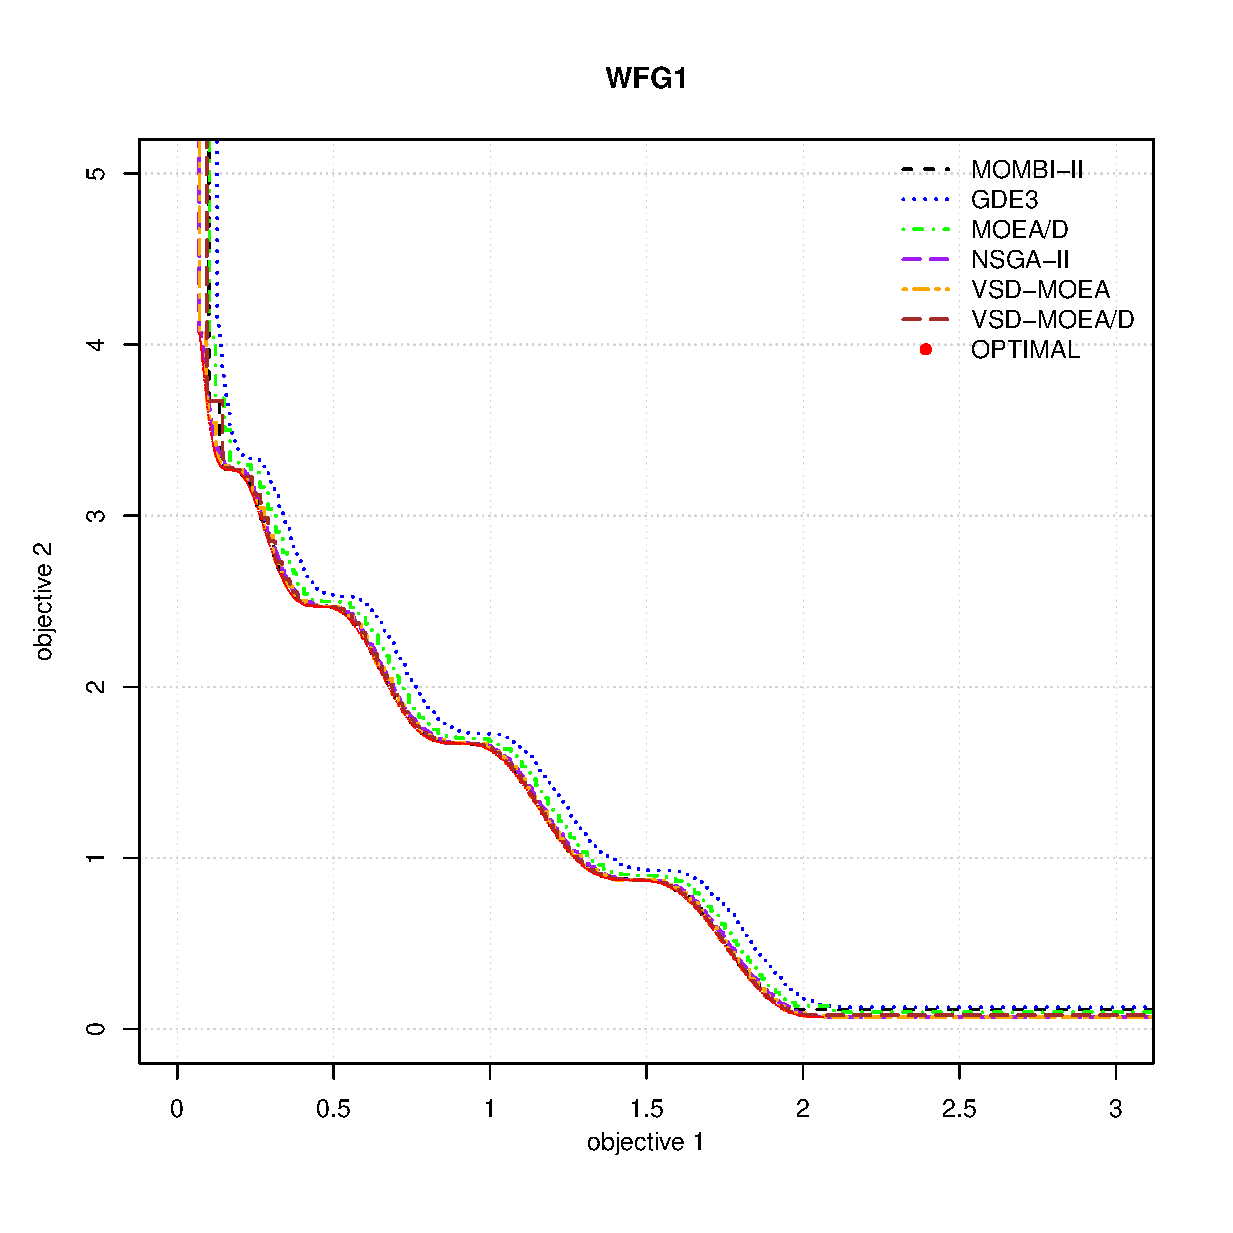
\includegraphics[width=0.33\textwidth]{Figures_Chapter7/Results_Chapter4/Surface_Representative/WFG1.eps}  &
  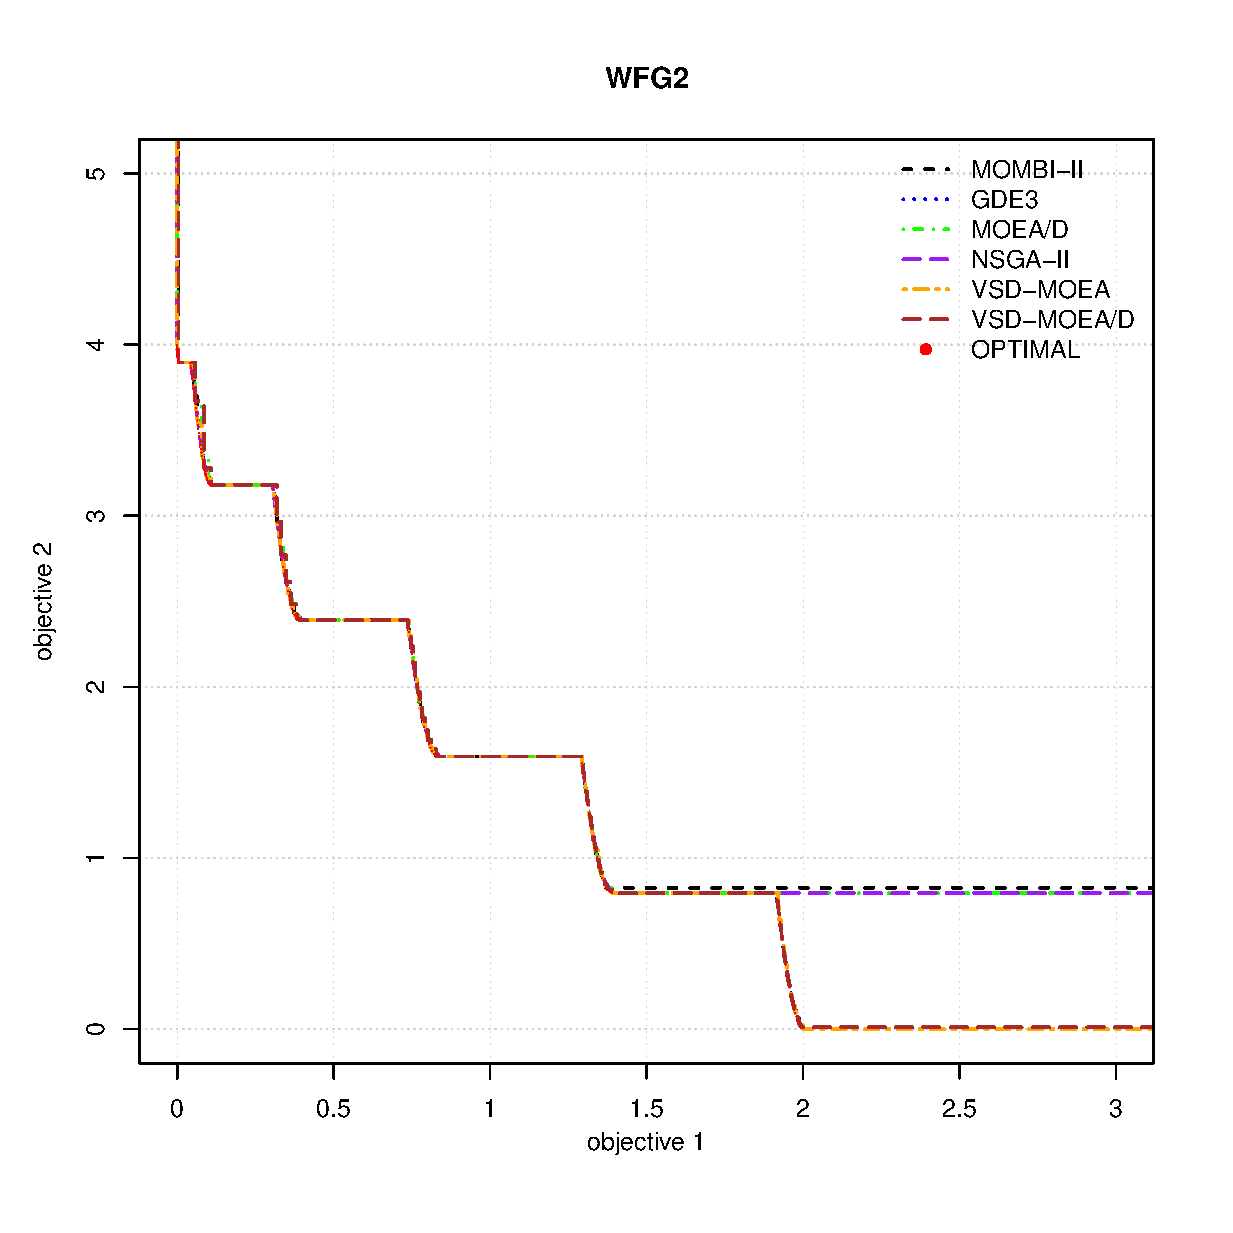
\includegraphics[width=0.33\textwidth]{Figures_Chapter7/Results_Chapter4/Surface_Representative/WFG2.eps} &
  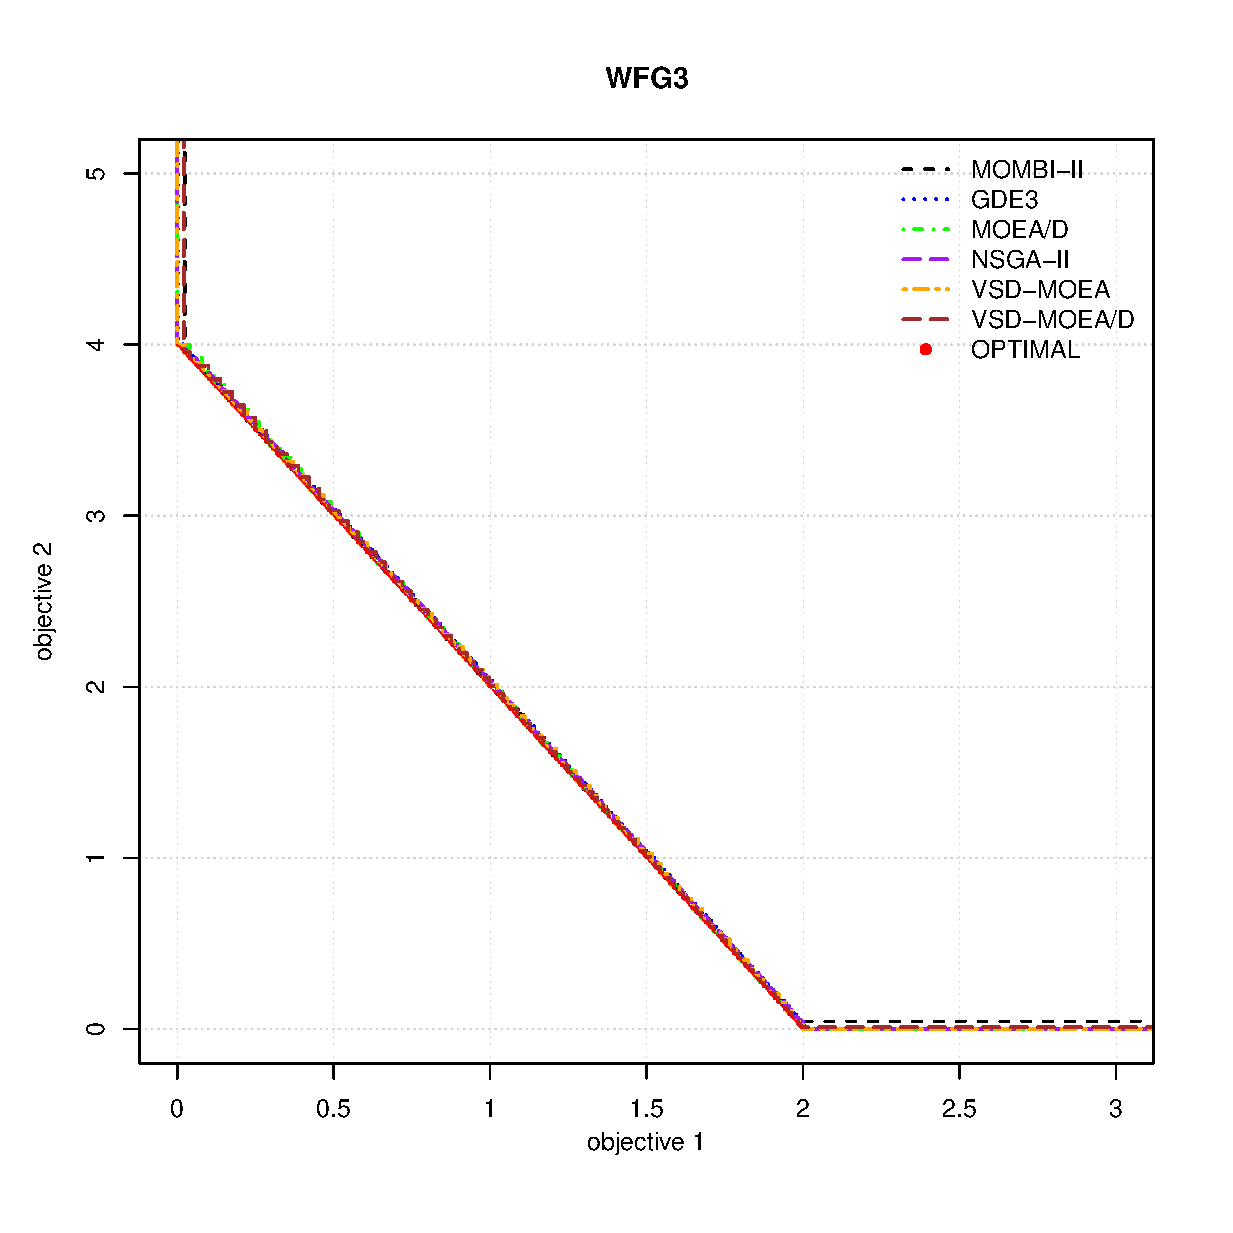
\includegraphics[width=0.33\textwidth]{Figures_Chapter7/Results_Chapter4/Surface_Representative/WFG3.eps} \\
  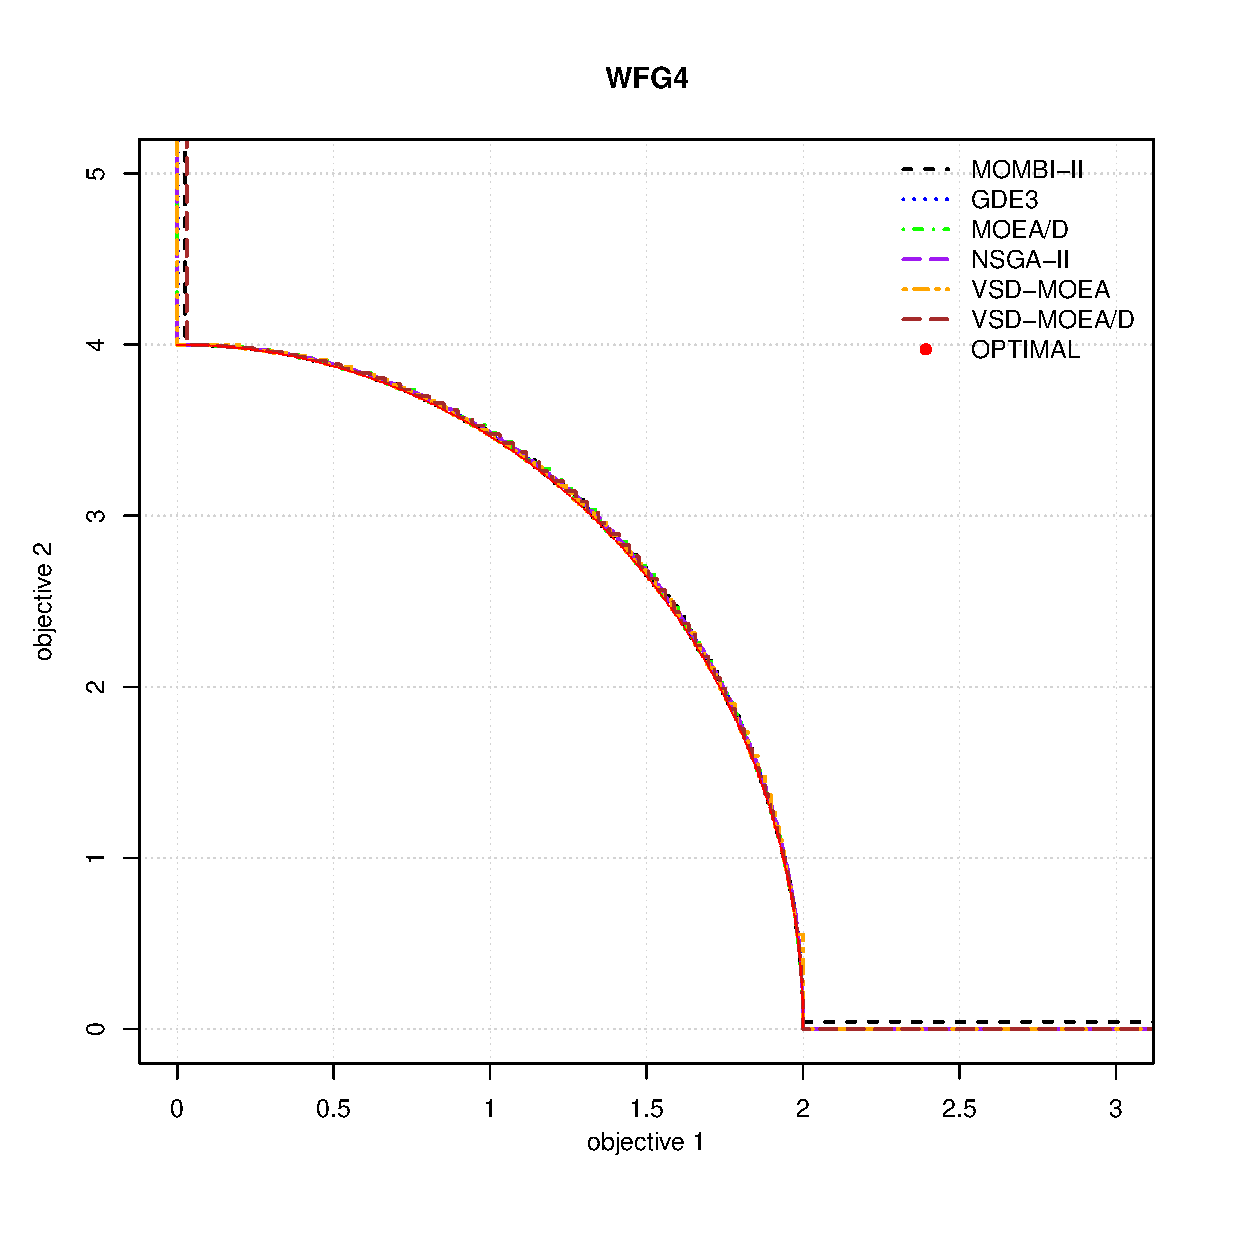
\includegraphics[width=0.33\textwidth]{Figures_Chapter7/Results_Chapter4/Surface_Representative/WFG4.eps} &
  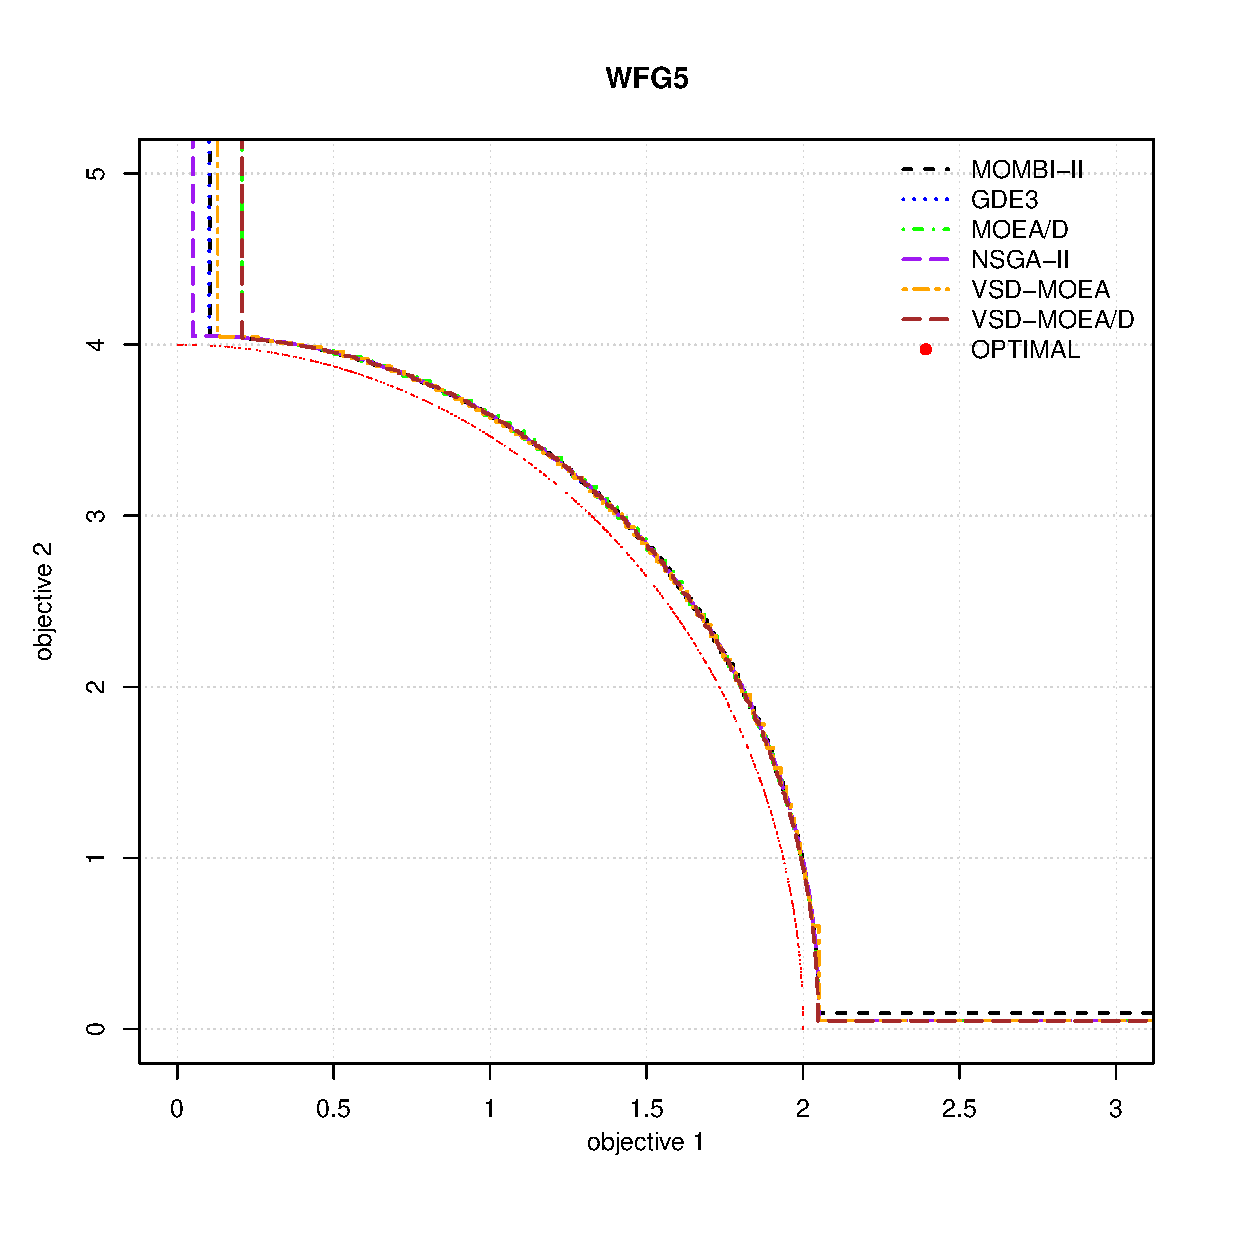
\includegraphics[width=0.33\textwidth]{Figures_Chapter7/Results_Chapter4/Surface_Representative/WFG5.eps} &
  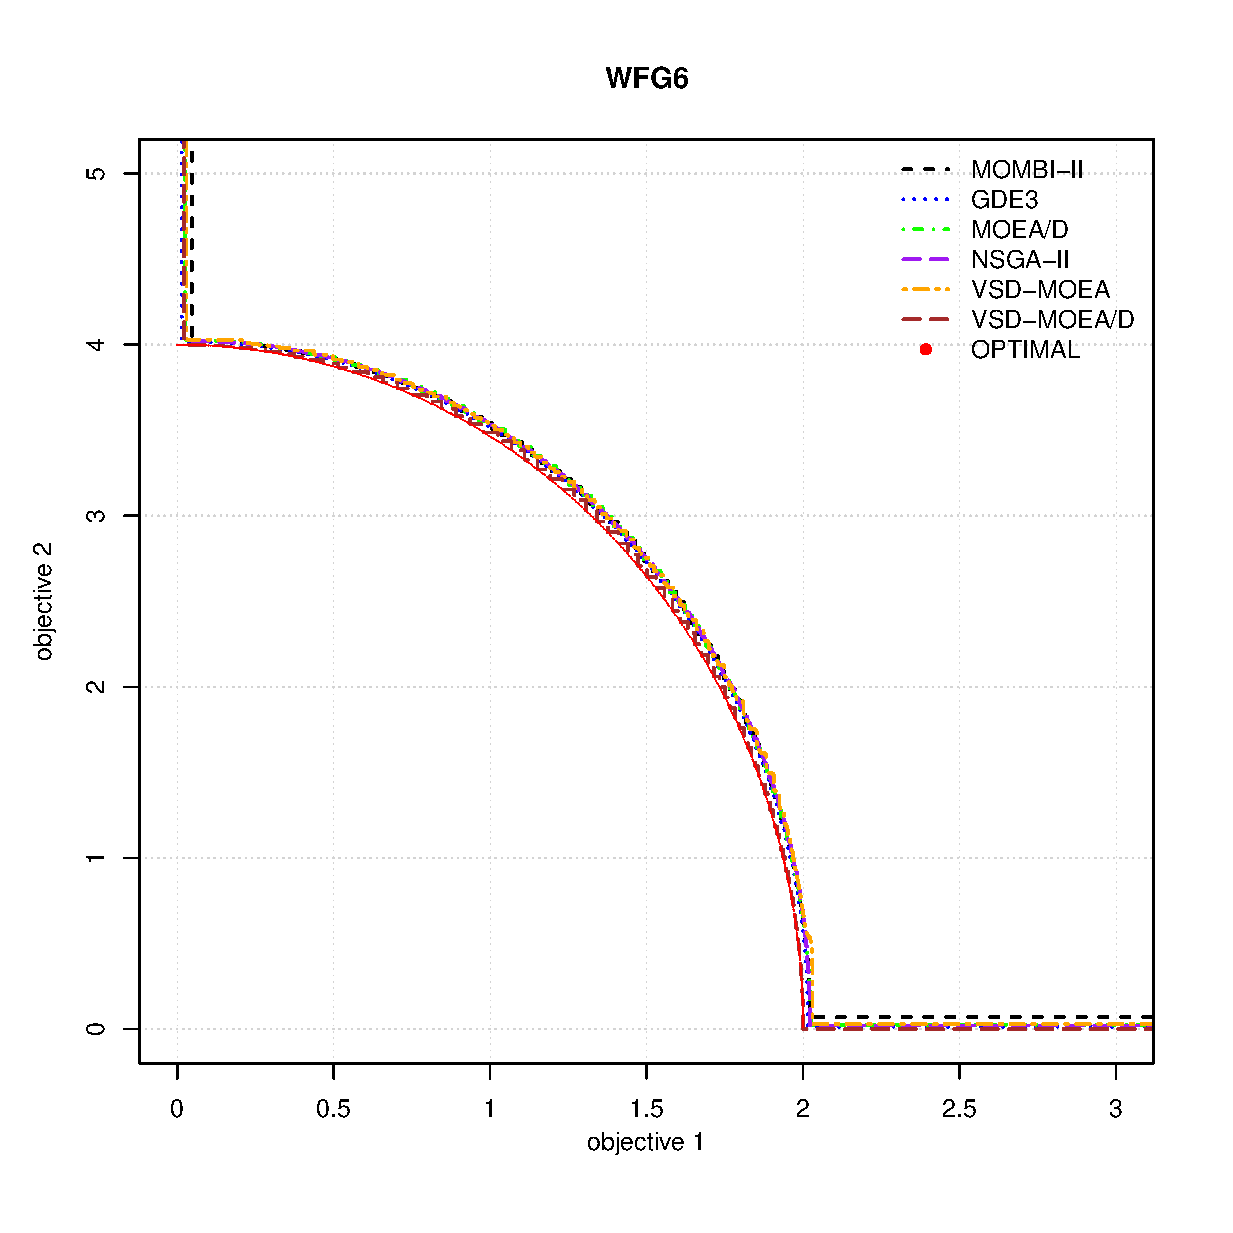
\includegraphics[width=0.33\textwidth]{Figures_Chapter7/Results_Chapter4/Surface_Representative/WFG6.eps} \\
  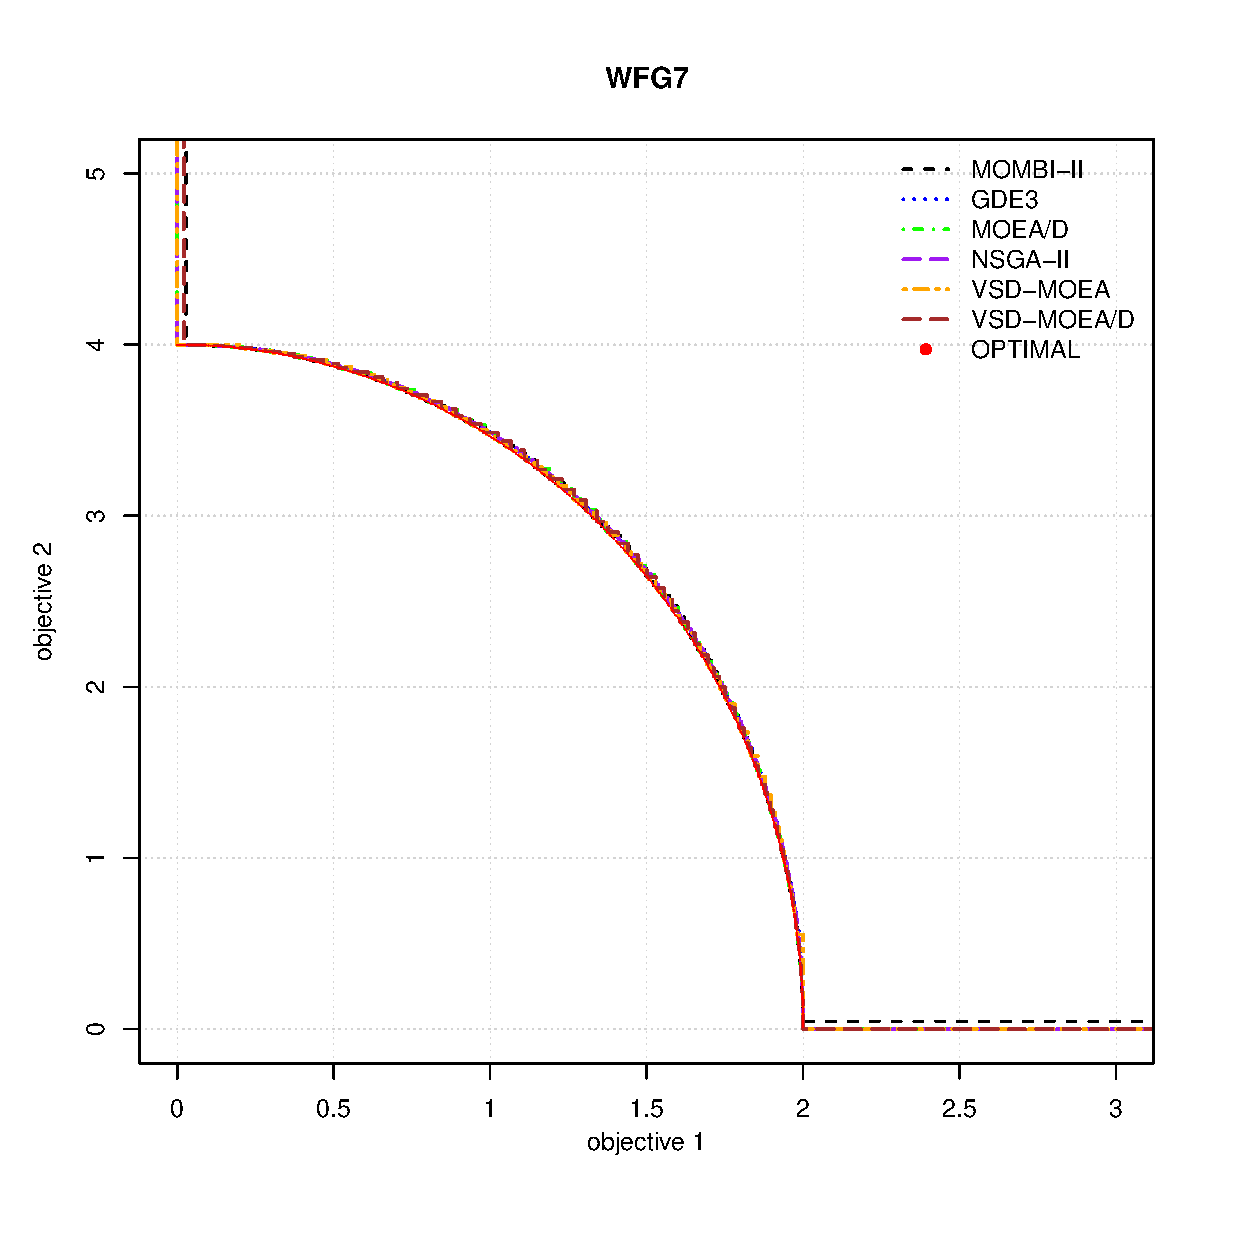
\includegraphics[width=0.33\textwidth]{Figures_Chapter7/Results_Chapter4/Surface_Representative/WFG7.eps} &
  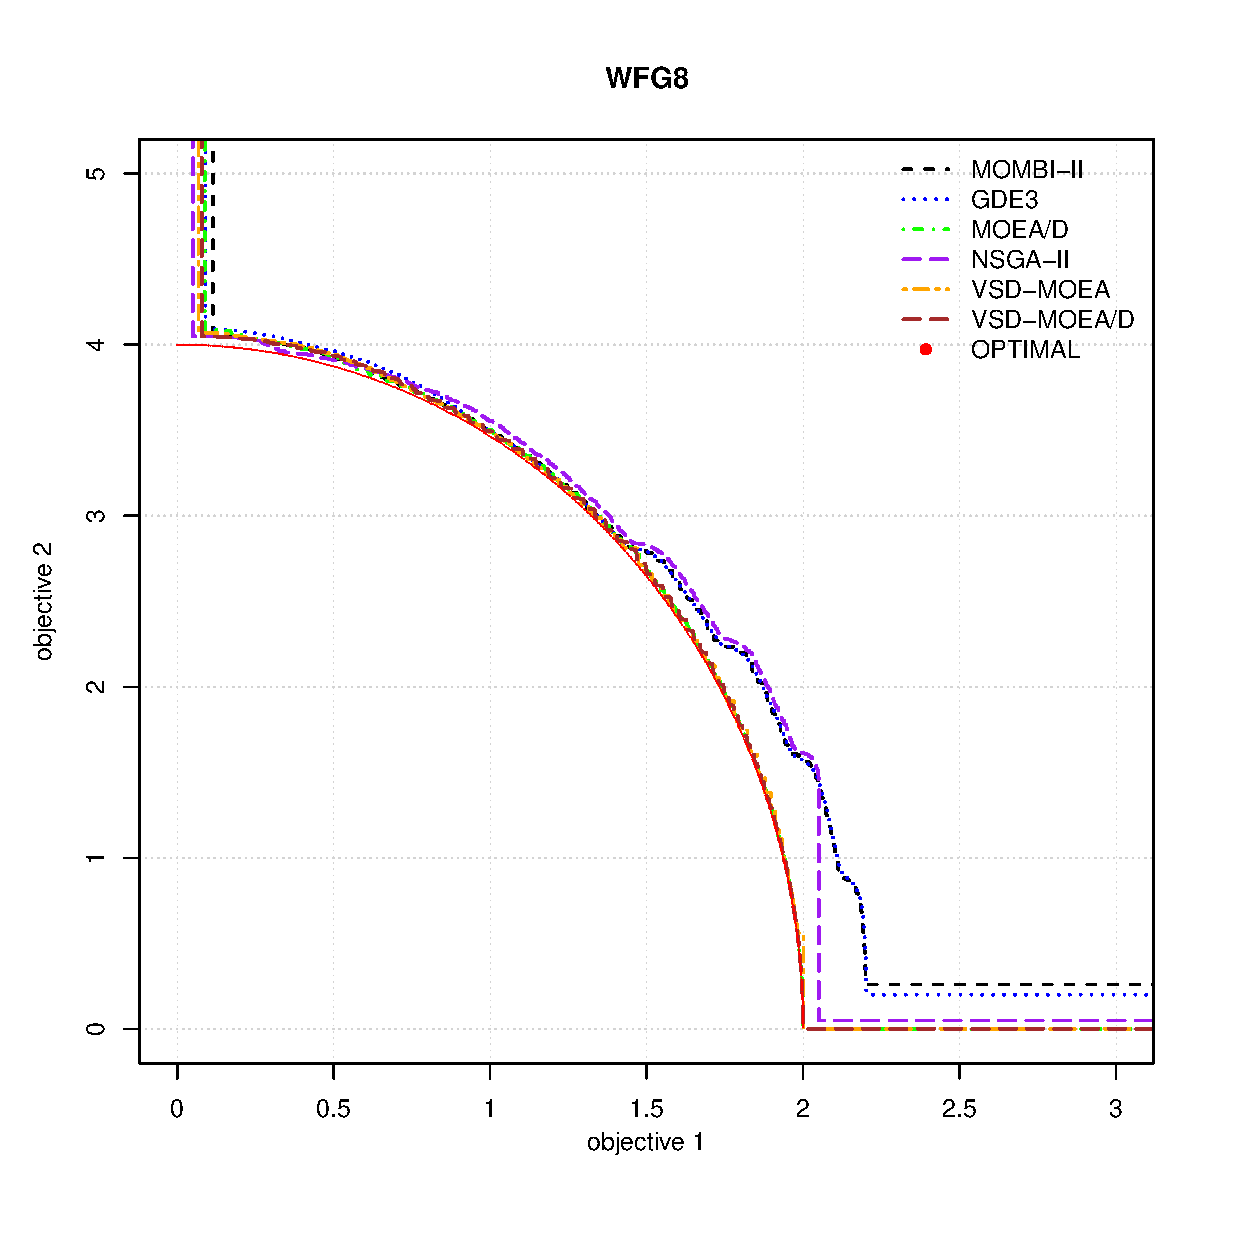
\includegraphics[width=0.33\textwidth]{Figures_Chapter7/Results_Chapter4/Surface_Representative/WFG8.eps} &
  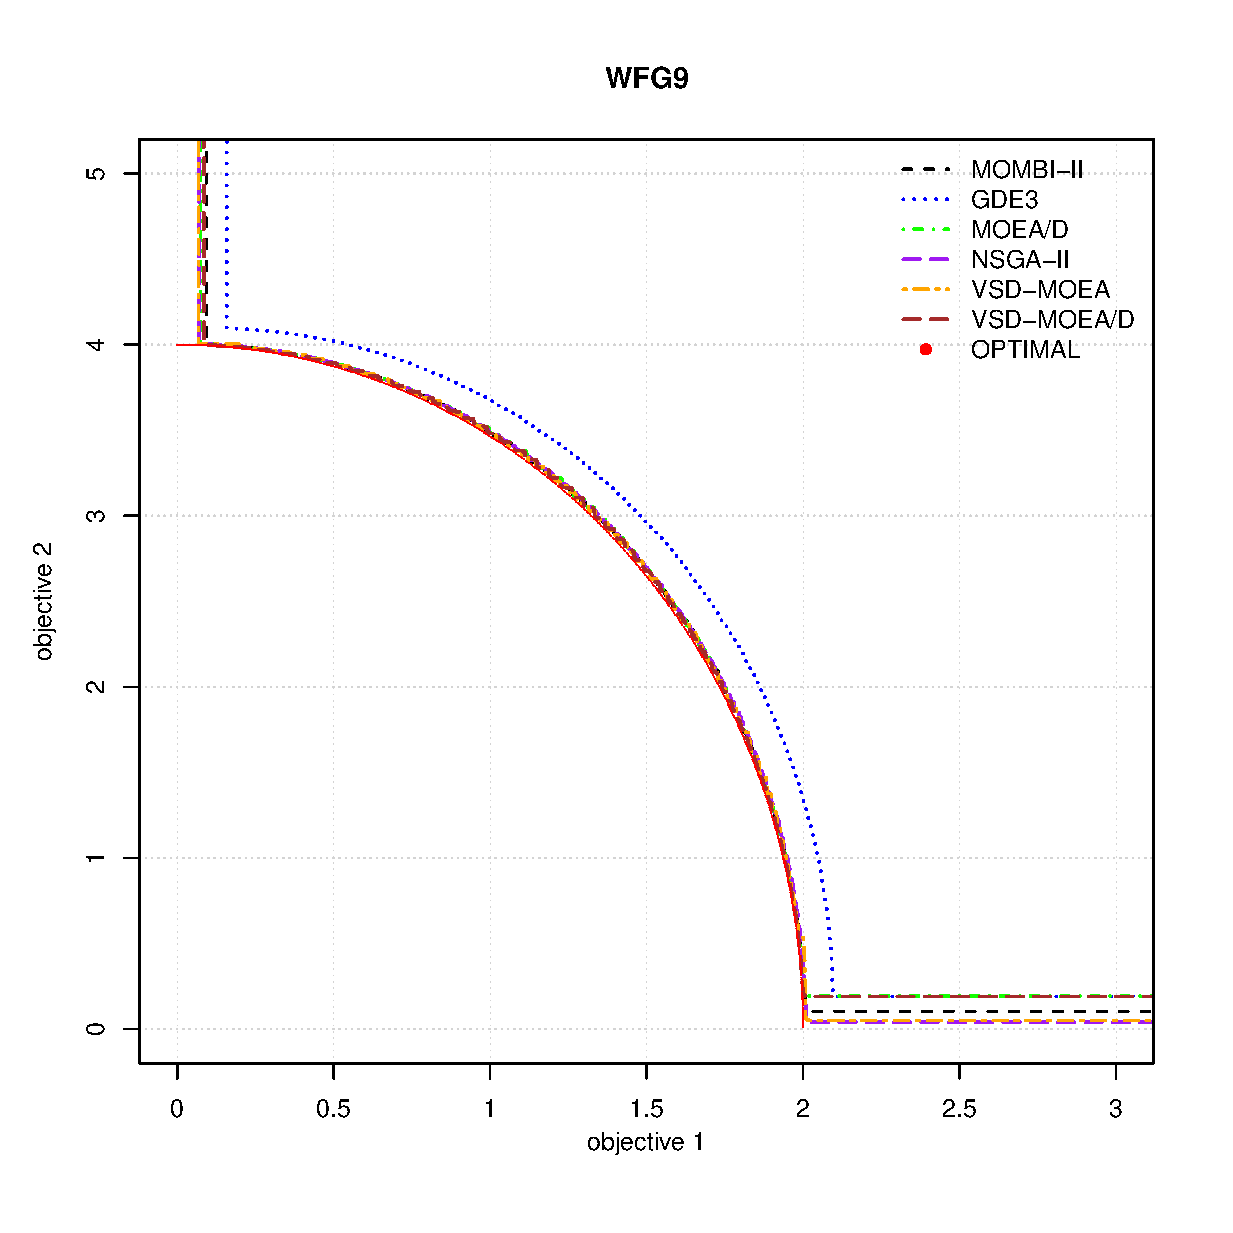
\includegraphics[width=0.33\textwidth]{Figures_Chapter7/Results_Chapter4/Surface_Representative/WFG9.eps}
\end{tabular}
\end{figure}
\begin{figure}[H]
%%\centering
\caption{superficies de cubrimiento logradas al 50\%}%Attainment Figures\_Chapter7 Achieved}
\begin{tabular}{ccc}
  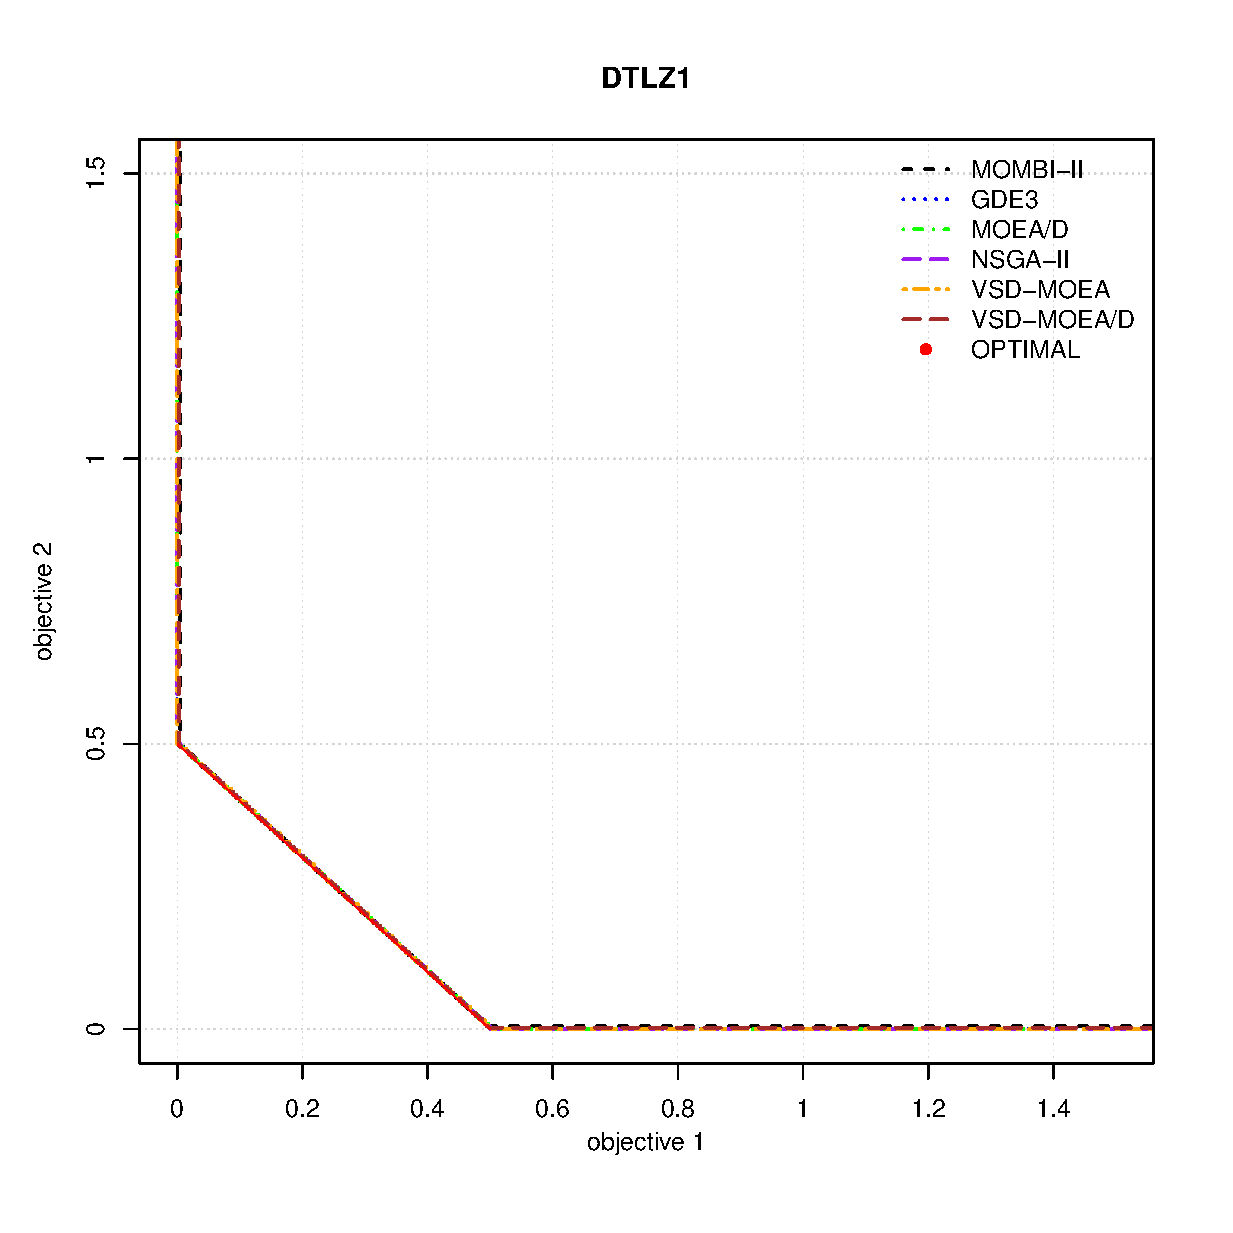
\includegraphics[width=0.33\textwidth]{Figures_Chapter7/Results_Chapter4/Surface_Representative/DTLZ1.eps}  &
  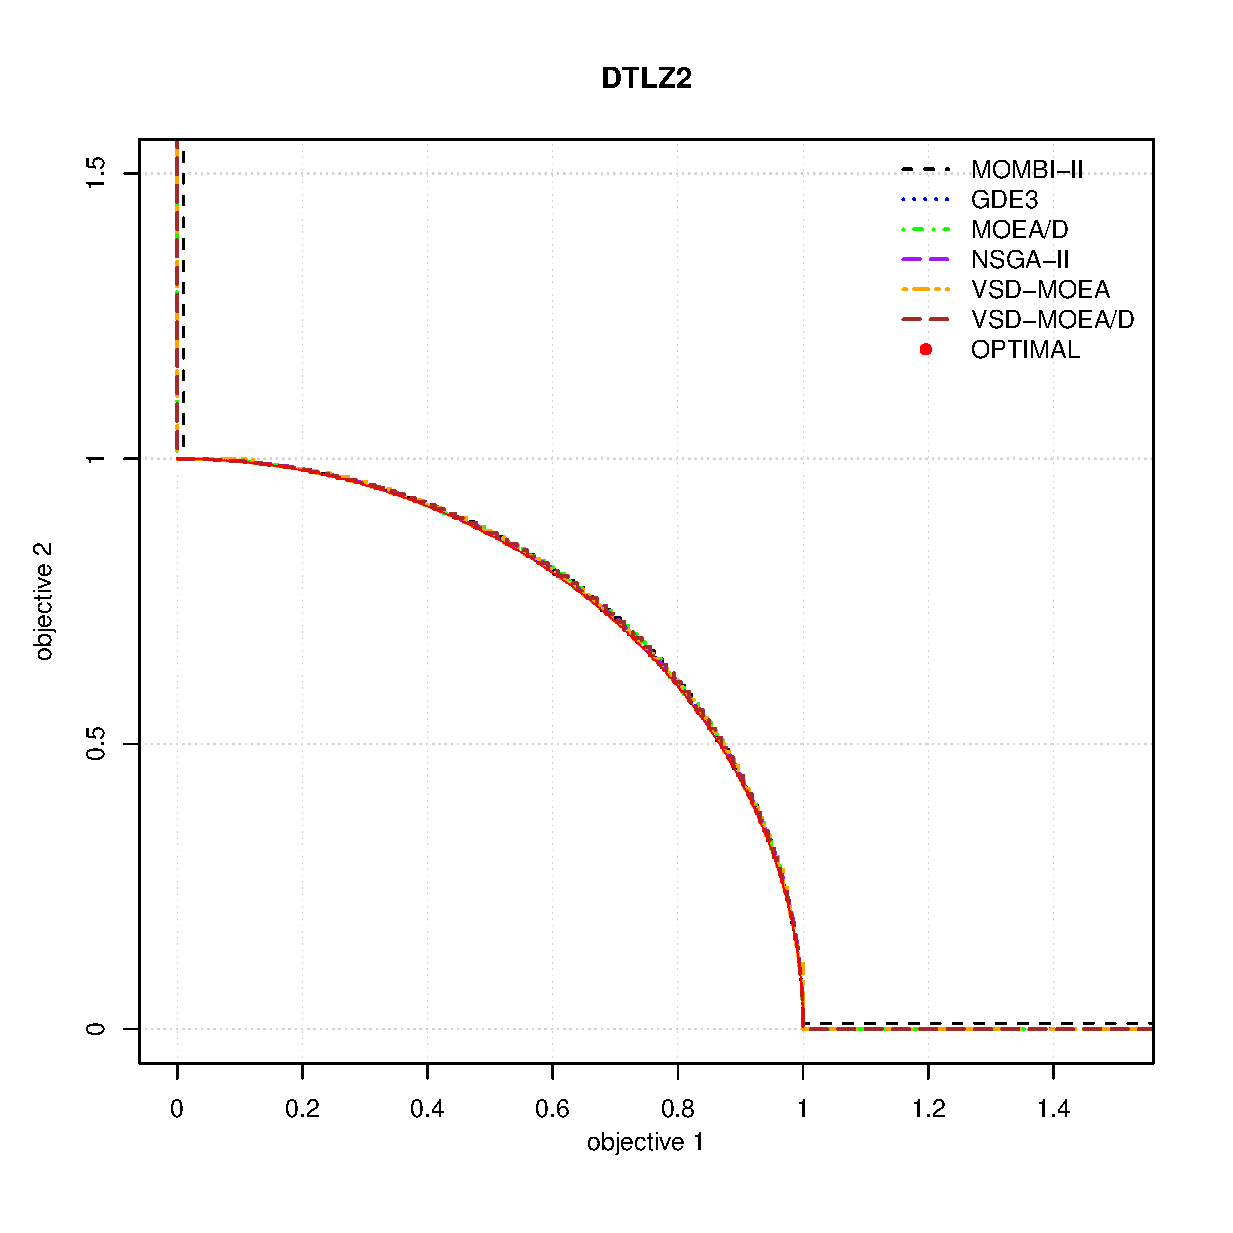
\includegraphics[width=0.33\textwidth]{Figures_Chapter7/Results_Chapter4/Surface_Representative/DTLZ2.eps} &
  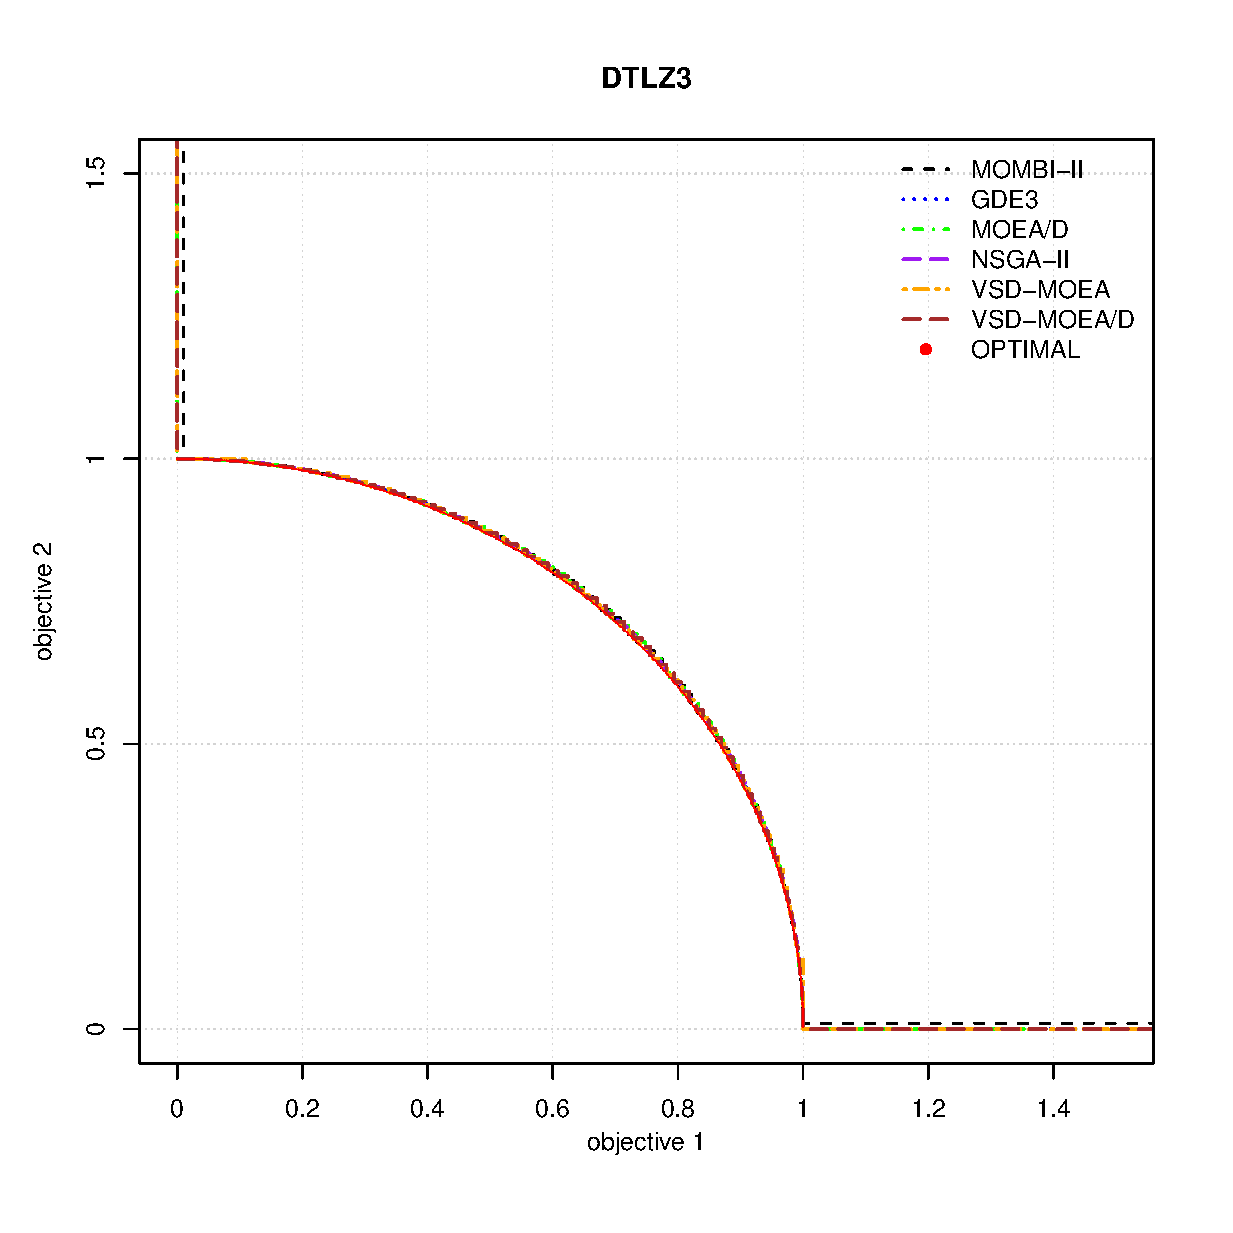
\includegraphics[width=0.33\textwidth]{Figures_Chapter7/Results_Chapter4/Surface_Representative/DTLZ3.eps} \\
  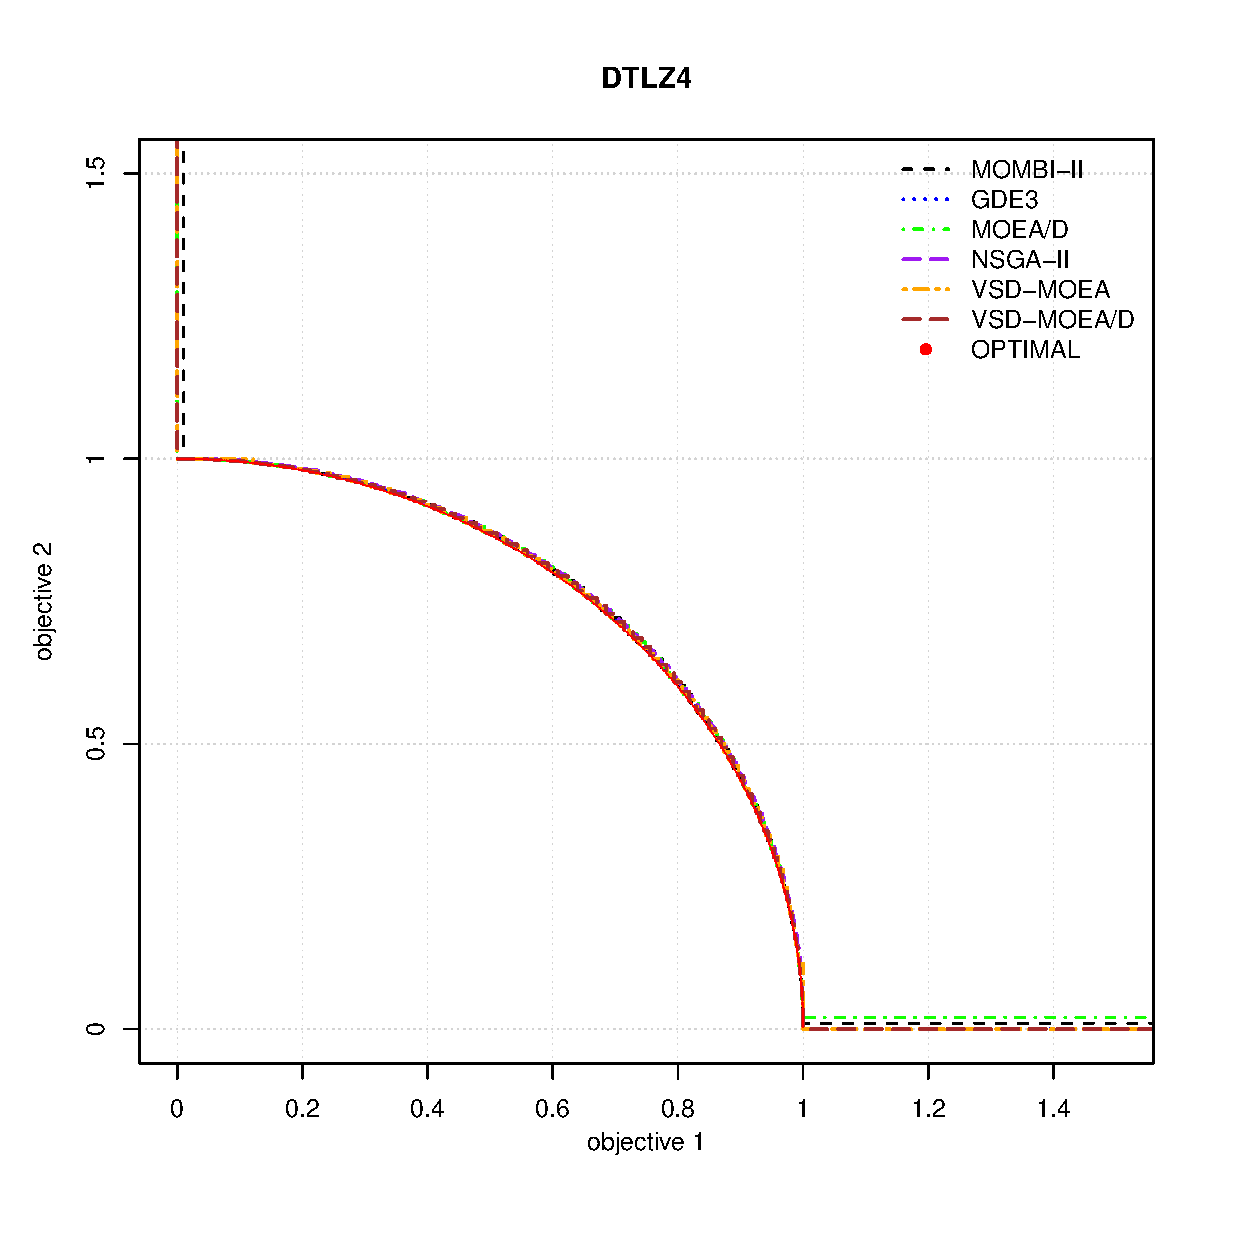
\includegraphics[width=0.33\textwidth]{Figures_Chapter7/Results_Chapter4/Surface_Representative/DTLZ4.eps} &
  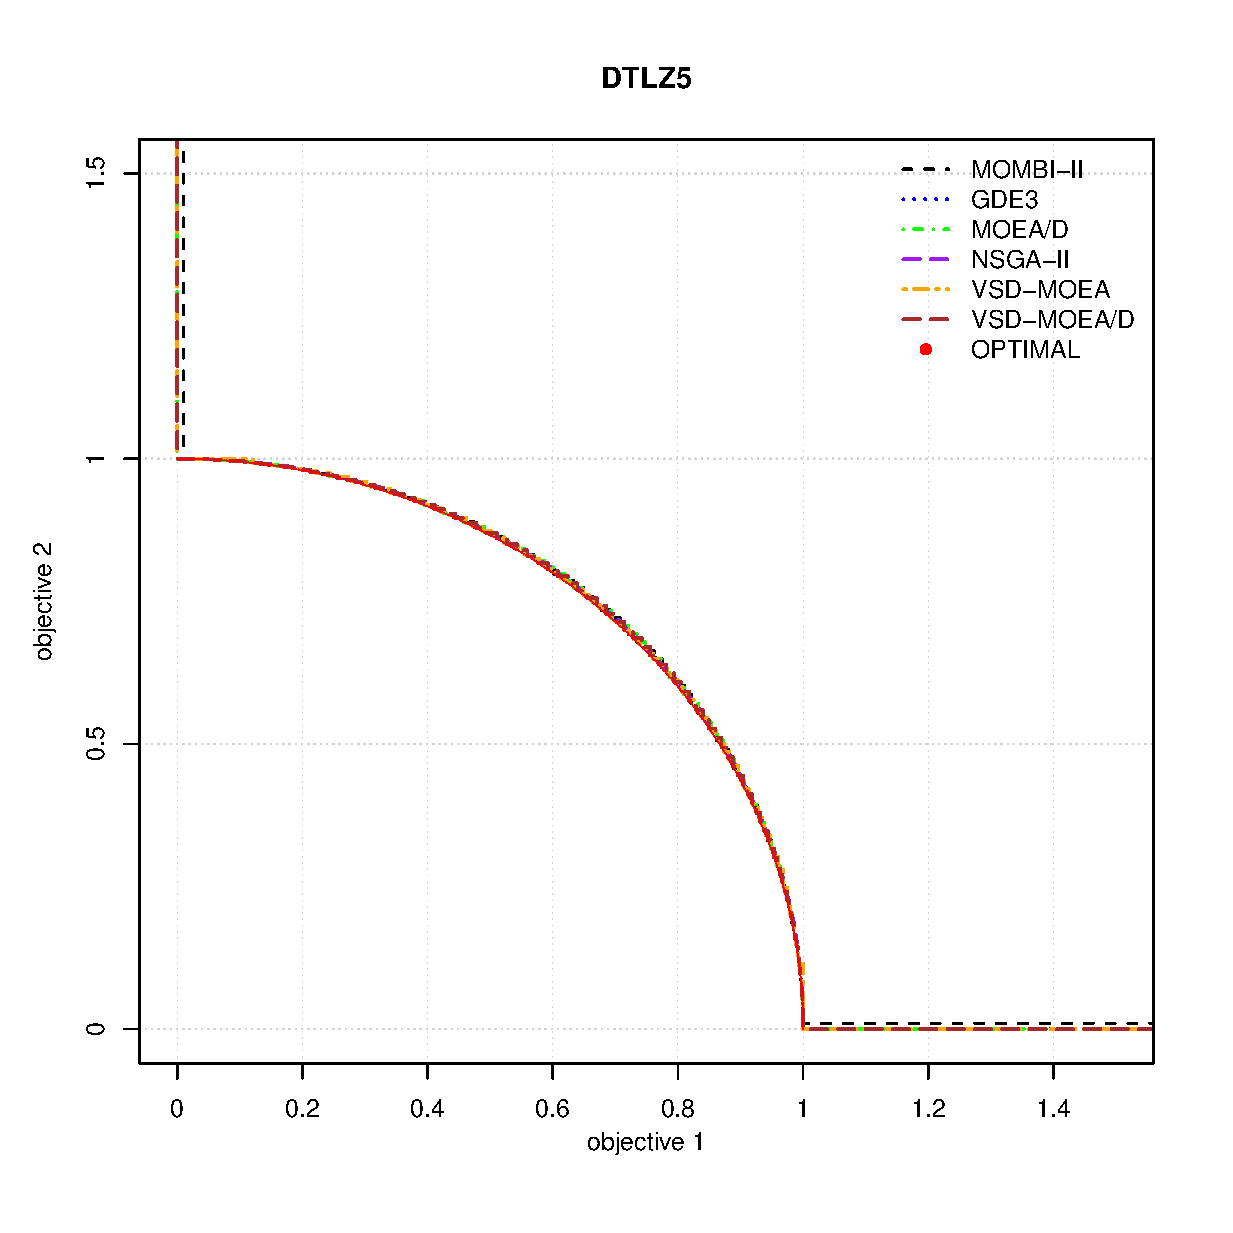
\includegraphics[width=0.33\textwidth]{Figures_Chapter7/Results_Chapter4/Surface_Representative/DTLZ5.eps} &
  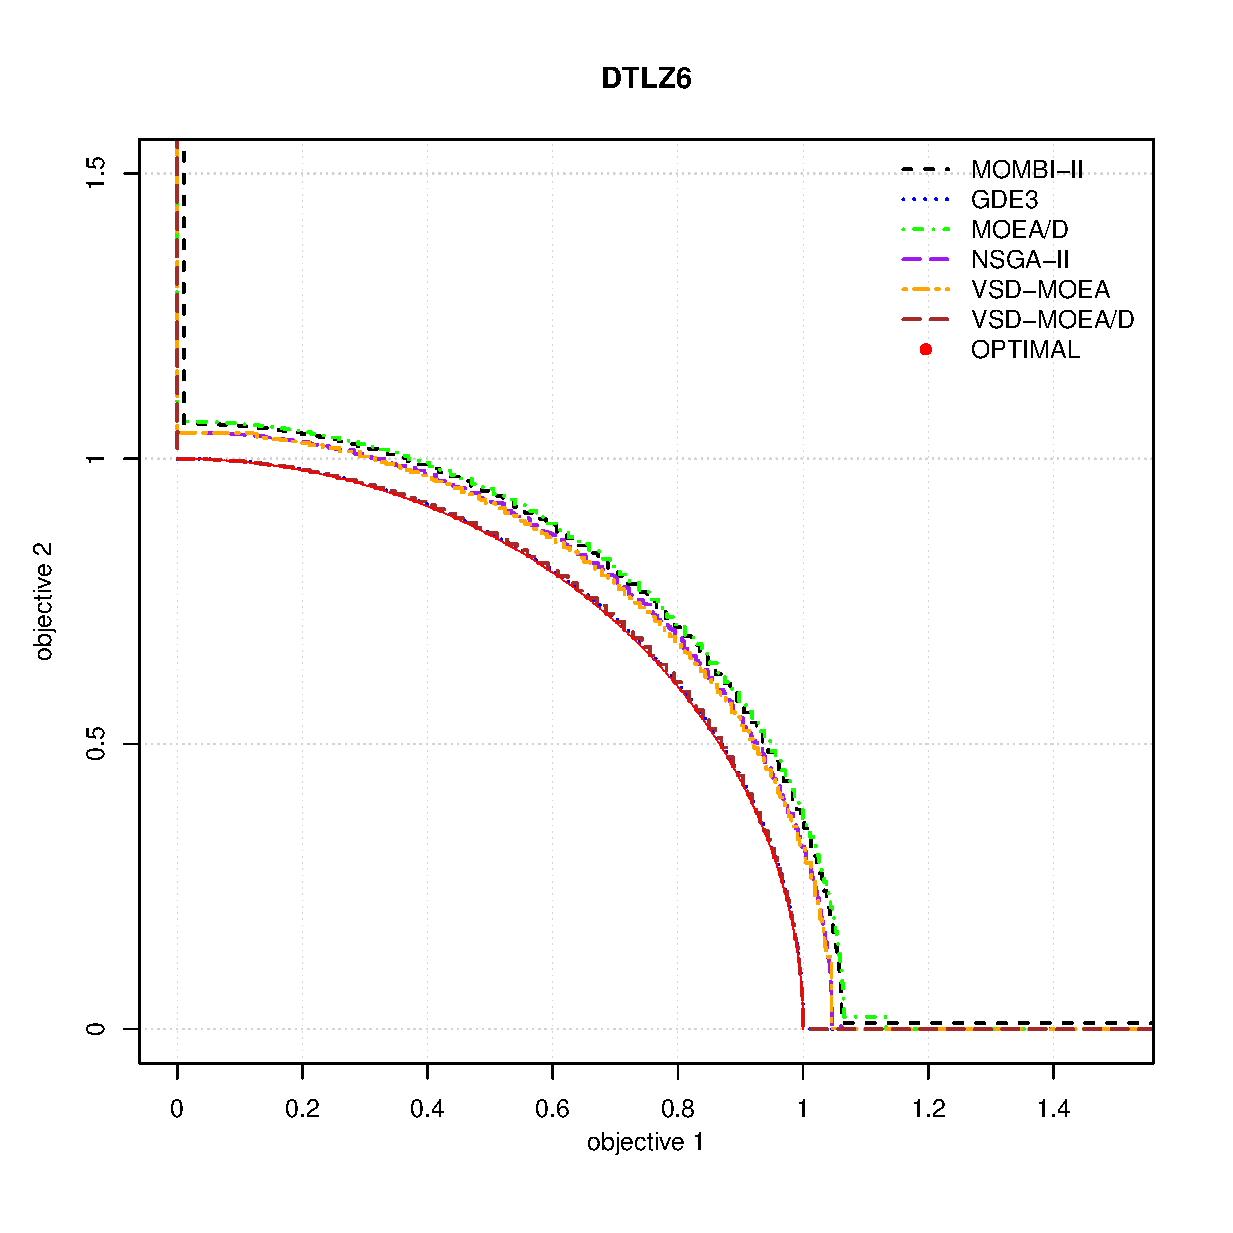
\includegraphics[width=0.33\textwidth]{Figures_Chapter7/Results_Chapter4/Surface_Representative/DTLZ6.eps} \\
  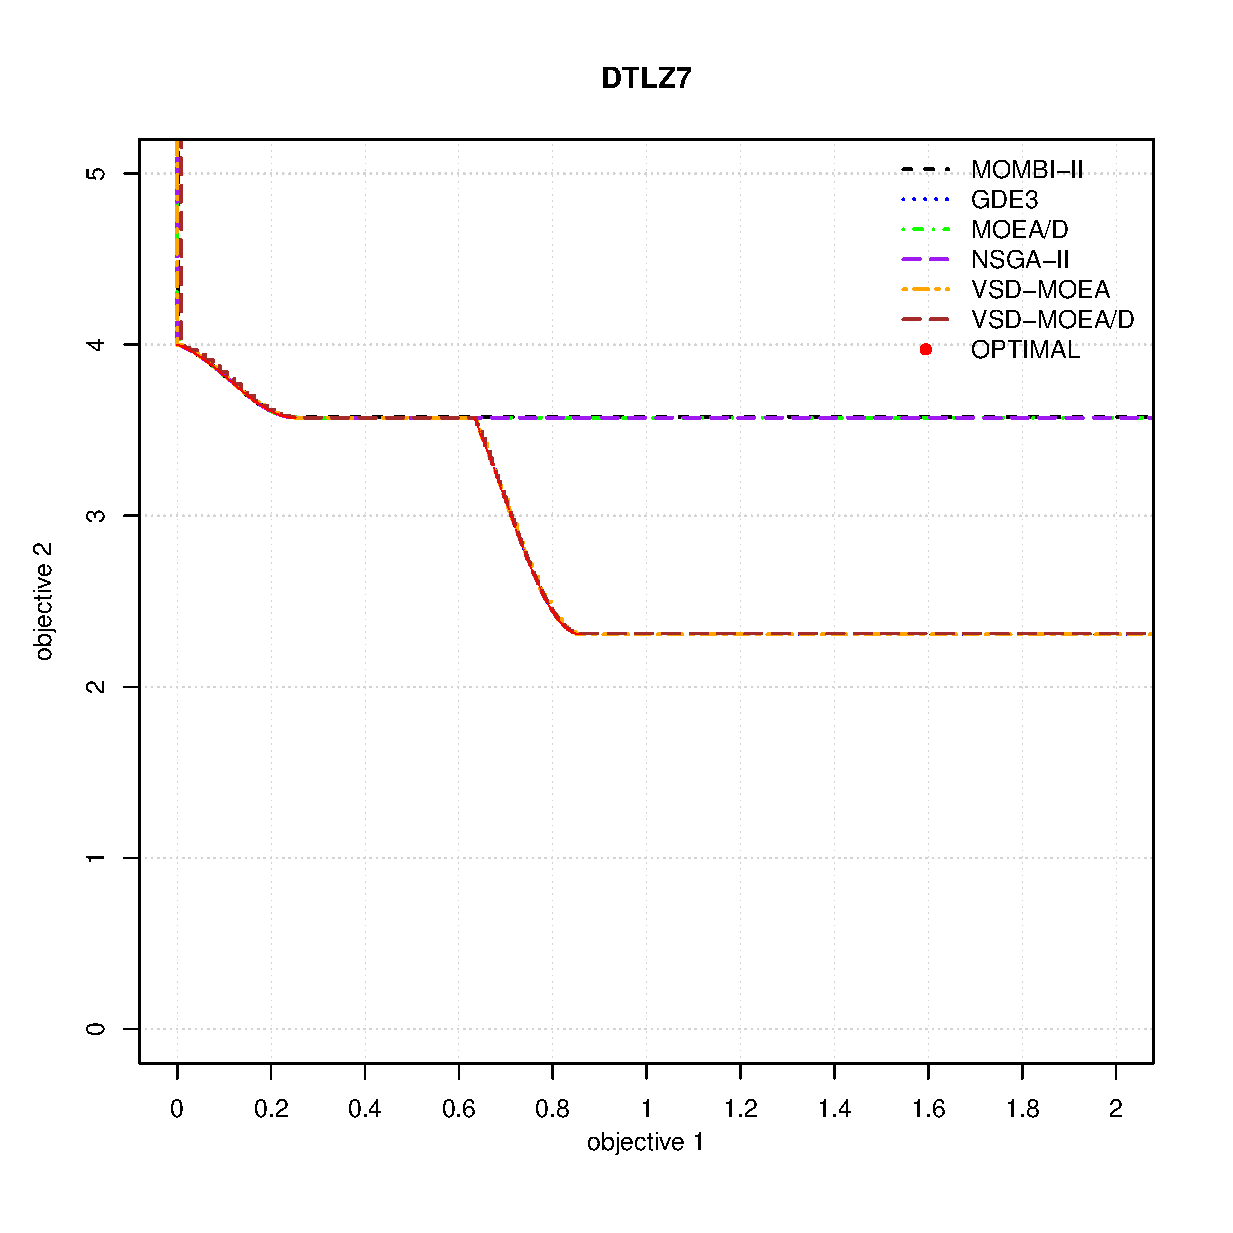
\includegraphics[width=0.33\textwidth]{Figures_Chapter7/Results_Chapter4/Surface_Representative/DTLZ7.eps} 
\end{tabular}
\end{figure}

\begin{figure}[H]
%%\centering
\caption{superficies de cubrimiento logradas al 50\%}%Attainment Figures\_Chapter7 Achieved}
\begin{tabular}{ccc}
  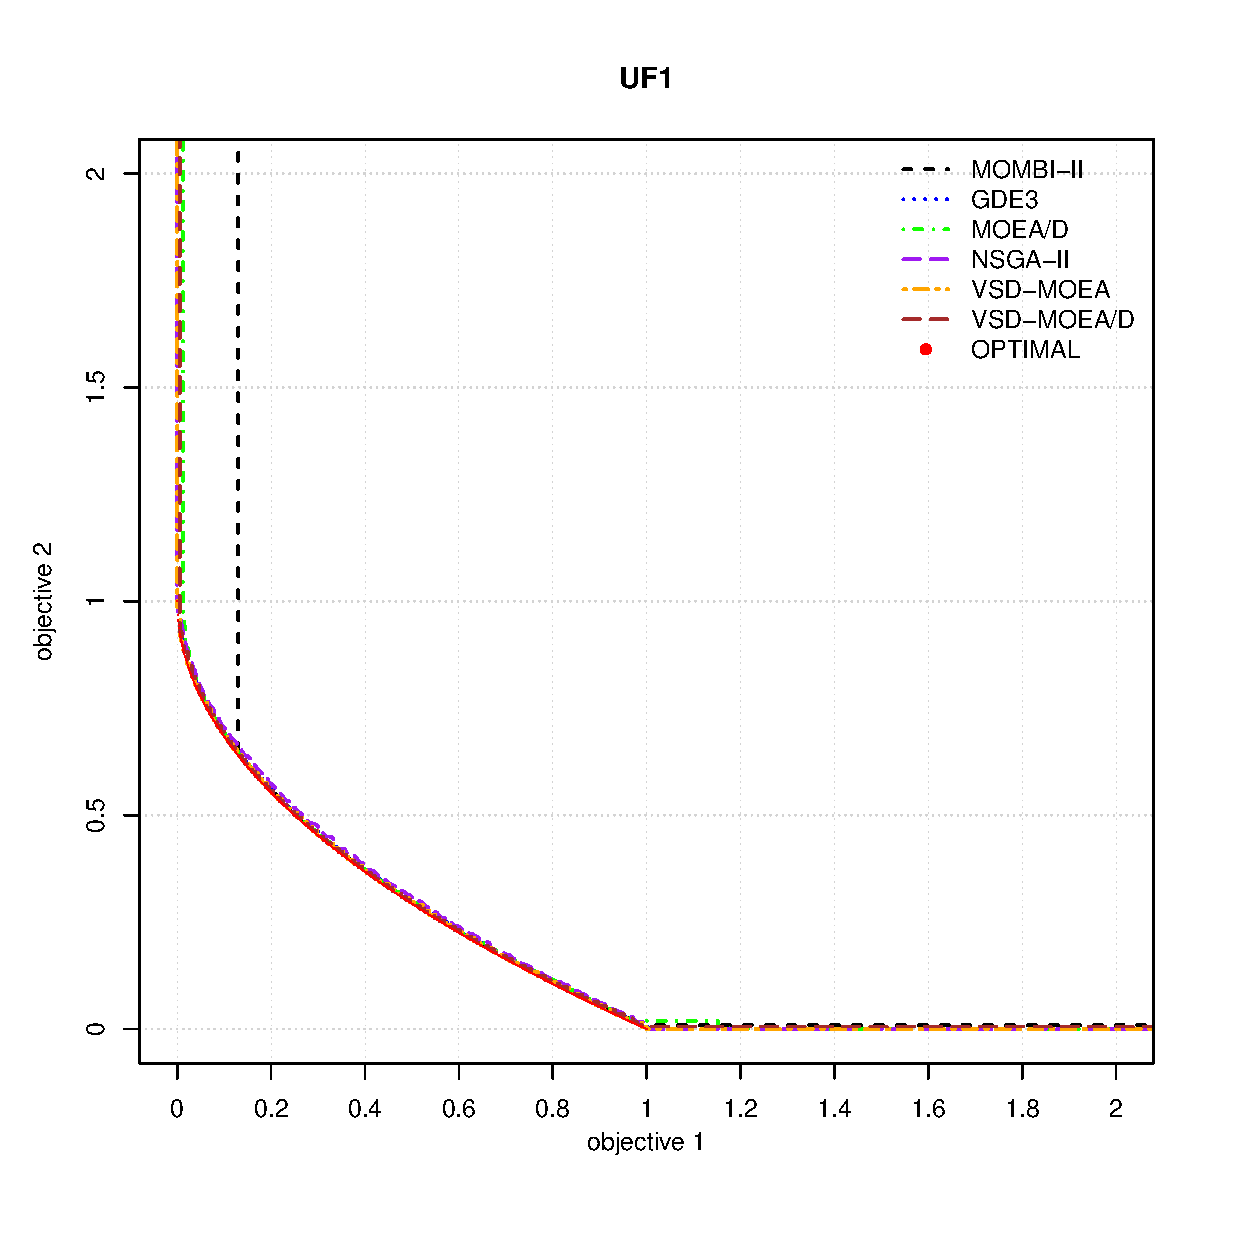
\includegraphics[width=0.33\textwidth]{Figures_Chapter7/Results_Chapter4/Surface_Representative/UF1.eps}  &
  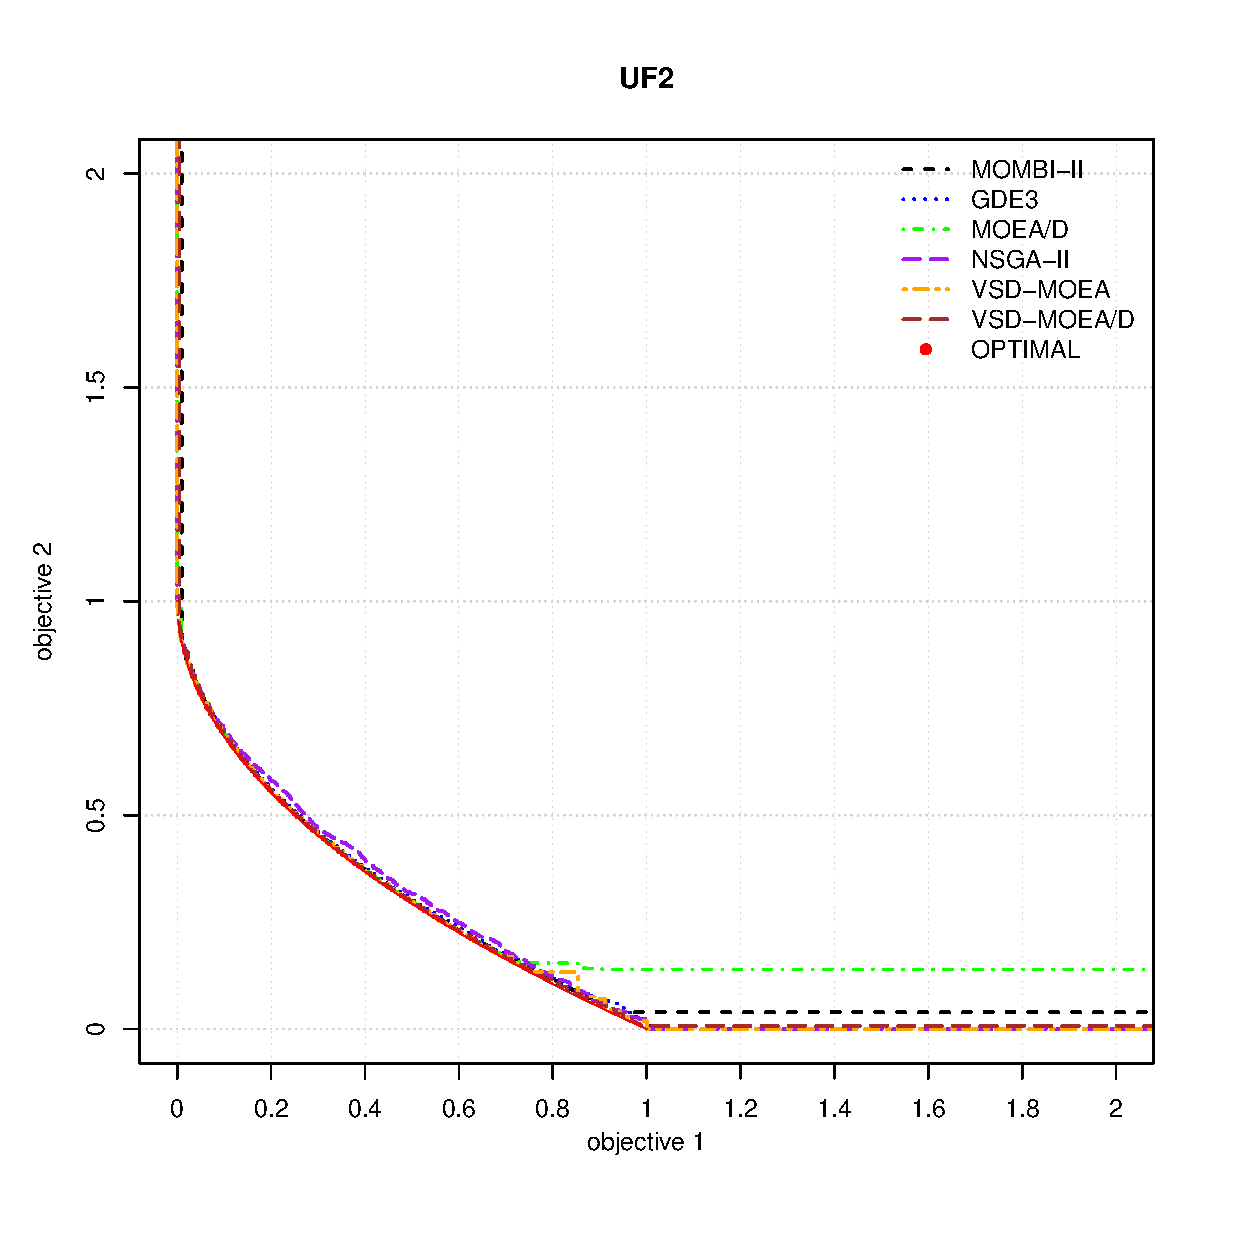
\includegraphics[width=0.33\textwidth]{Figures_Chapter7/Results_Chapter4/Surface_Representative/UF2.eps} &
  \includegraphics[width=0.33\textwidth]{Figures_Chapter7/Results_Chapter4/Surface_Representative/UF3.eps} \\
  \includegraphics[width=0.33\textwidth]{Figures_Chapter7/Results_Chapter4/Surface_Representative/UF4.eps} &
  \includegraphics[width=0.33\textwidth]{Figures_Chapter7/Results_Chapter4/Surface_Representative/UF5.eps} &
  \includegraphics[width=0.33\textwidth]{Figures_Chapter7/Results_Chapter4/Surface_Representative/UF6.eps} \\
  \includegraphics[width=0.33\textwidth]{Figures_Chapter7/Results_Chapter4/Surface_Representative/UF7.eps} 
\end{tabular}
\end{figure}


%///////////////
\begin{figure}[H]
\centering
\scriptsize
\caption{Frente no dominado de las 35 ejecuciones, en la columna izquierda el VSD-MOEA y la derecha el VSD-MOEA/D}%Attainment Figures\_Chapter7 Achieved}
\begin{tabular}{cc}
  \includegraphics[scale=0.3, angle=-90,origin=c]{Figures_Chapter7/Results_Chapter4/Summary_Representative/VSD-MOEA/WFG1.eps}  &
  \includegraphics[scale=0.3, angle=-90,origin=c]{Figures_Chapter7/Results_Chapter4/Summary_Representative/VSD-MOEA-D/WFG1.eps}  \\
  \includegraphics[scale=0.3, angle=-90,origin=c]{Figures_Chapter7/Results_Chapter4/Summary_Representative/VSD-MOEA/WFG2.eps} &
  \includegraphics[scale=0.3, angle=-90,origin=c]{Figures_Chapter7/Results_Chapter4/Summary_Representative/VSD-MOEA-D/WFG2.eps} \\
  \includegraphics[scale=0.3, angle=-90,origin=c]{Figures_Chapter7/Results_Chapter4/Summary_Representative/VSD-MOEA/WFG3.eps} &
  \includegraphics[scale=0.3, angle=-90,origin=c]{Figures_Chapter7/Results_Chapter4/Summary_Representative/VSD-MOEA-D/WFG3.eps} \\
  \includegraphics[scale=0.3, angle=-90,origin=c]{Figures_Chapter7/Results_Chapter4/Summary_Representative/VSD-MOEA/WFG4.eps} &
  \includegraphics[scale=0.3, angle=-90,origin=c]{Figures_Chapter7/Results_Chapter4/Summary_Representative/VSD-MOEA-D/WFG4.eps} 
%  \includegraphics[scale=0.3, angle=-90,origin=c]{Figures_Chapter7/Results_Chapter4/Summary_Representative/VSD-MOEA/WFG5.eps} &
%  \includegraphics[scale=0.3, angle=-90,origin=c]{Figures_Chapter7/Results_Chapter4/Summary_Representative/VSD-MOEA-D/WFG5.eps} \\
%  \includegraphics[scale=0.3, angle=-90,origin=c]{Figures_Chapter7/Results_Chapter4/Summary_Representative/VSD-MOEA/WFG6.eps} &
%  \includegraphics[scale=0.3, angle=-90,origin=c]{Figures_Chapter7/Results_Chapter4/Summary_Representative/VSD-MOEA-D/WFG6.eps} \\
%  \includegraphics[scale=0.3, angle=-90,origin=c]{Figures_Chapter7/Results_Chapter4/Summary_Representative/VSD-MOEA/WFG7.eps} &
%  \includegraphics[scale=0.3, angle=-90,origin=c]{Figures_Chapter7/Results_Chapter4/Summary_Representative/VSD-MOEA-D/WFG7.eps} \\
%  \includegraphics[scale=0.3, angle=-90,origin=c]{Figures_Chapter7/Results_Chapter4/Summary_Representative/VSD-MOEA/WFG8.eps} &
%  \includegraphics[scale=0.3, angle=-90,origin=c]{Figures_Chapter7/Results_Chapter4/Summary_Representative/VSD-MOEA-D/WFG8.eps} \\
%  \includegraphics[scale=0.3, angle=-90,origin=c]{Figures_Chapter7/Results_Chapter4/Summary_Representative/VSD-MOEA/WFG9.eps} &
%  \includegraphics[scale=0.3, angle=-90,origin=c]{Figures_Chapter7/Results_Chapter4/Summary_Representative/VSD-MOEA-D/WFG9.eps}
\end{tabular}
\end{figure}

\begin{figure}[H]
\centering
\scriptsize
\caption{Frente no dominado de las 35 ejecuciones, en la columna izquierda el VSD-MOEA y la derecha el VSD-MOEA/D}%Attainment Figures\_Chapter7 Achieved}
\begin{tabular}{cc}
%  \includegraphics[scale=0.3, angle=-90,origin=c]{Figures_Chapter7/Results_Chapter4/Summary_Representative/VSD-MOEA/WFG1.eps}  &
%  \includegraphics[scale=0.3, angle=-90,origin=c]{Figures_Chapter7/Results_Chapter4/Summary_Representative/VSD-MOEA-D/WFG1.eps}  \\
%  \includegraphics[scale=0.3, angle=-90,origin=c]{Figures_Chapter7/Results_Chapter4/Summary_Representative/VSD-MOEA/WFG2.eps} &
%  \includegraphics[scale=0.3, angle=-90,origin=c]{Figures_Chapter7/Results_Chapter4/Summary_Representative/VSD-MOEA-D/WFG2.eps} \\
%  \includegraphics[scale=0.3, angle=-90,origin=c]{Figures_Chapter7/Results_Chapter4/Summary_Representative/VSD-MOEA/WFG3.eps} &
%  \includegraphics[scale=0.3, angle=-90,origin=c]{Figures_Chapter7/Results_Chapter4/Summary_Representative/VSD-MOEA-D/WFG3.eps} \\
%  \includegraphics[scale=0.3, angle=-90,origin=c]{Figures_Chapter7/Results_Chapter4/Summary_Representative/VSD-MOEA/WFG4.eps} &
%  \includegraphics[scale=0.3, angle=-90,origin=c]{Figures_Chapter7/Results_Chapter4/Summary_Representative/VSD-MOEA-D/WFG4.eps} \\
  \includegraphics[scale=0.3, angle=-90,origin=c]{Figures_Chapter7/Results_Chapter4/Summary_Representative/VSD-MOEA/WFG5.eps} &
  \includegraphics[scale=0.3, angle=-90,origin=c]{Figures_Chapter7/Results_Chapter4/Summary_Representative/VSD-MOEA-D/WFG5.eps} \\
  \includegraphics[scale=0.3, angle=-90,origin=c]{Figures_Chapter7/Results_Chapter4/Summary_Representative/VSD-MOEA/WFG6.eps} &
  \includegraphics[scale=0.3, angle=-90,origin=c]{Figures_Chapter7/Results_Chapter4/Summary_Representative/VSD-MOEA-D/WFG6.eps} \\
  \includegraphics[scale=0.3, angle=-90,origin=c]{Figures_Chapter7/Results_Chapter4/Summary_Representative/VSD-MOEA/WFG7.eps} &
  \includegraphics[scale=0.3, angle=-90,origin=c]{Figures_Chapter7/Results_Chapter4/Summary_Representative/VSD-MOEA-D/WFG7.eps} \\
  \includegraphics[scale=0.3, angle=-90,origin=c]{Figures_Chapter7/Results_Chapter4/Summary_Representative/VSD-MOEA/WFG8.eps} &
  \includegraphics[scale=0.3, angle=-90,origin=c]{Figures_Chapter7/Results_Chapter4/Summary_Representative/VSD-MOEA-D/WFG8.eps} 
%  \includegraphics[scale=0.3, angle=-90,origin=c]{Figures_Chapter7/Results_Chapter4/Summary_Representative/VSD-MOEA/WFG9.eps} &
%  \includegraphics[scale=0.3, angle=-90,origin=c]{Figures_Chapter7/Results_Chapter4/Summary_Representative/VSD-MOEA-D/WFG9.eps}
\end{tabular}
\end{figure}

\begin{figure}[H]
\centering
\scriptsize
\caption{Frente no dominado de las 35 ejecuciones, en la columna izquierda el VSD-MOEA y la derecha el VSD-MOEA/D}%Attainment Figures\_Chapter7 Achieved}
\begin{tabular}{cc}
  \includegraphics[scale=0.3, angle=-90,origin=c]{Figures_Chapter7/Results_Chapter4/Summary_Representative/VSD-MOEA/WFG9.eps} &
  \includegraphics[scale=0.3, angle=-90,origin=c]{Figures_Chapter7/Results_Chapter4/Summary_Representative/VSD-MOEA-D/WFG9.eps} \\
  \includegraphics[scale=0.3, angle=-90,origin=c]{Figures_Chapter7/Results_Chapter4/Summary_Representative/VSD-MOEA/DTLZ1.eps}  &
  \includegraphics[scale=0.3, angle=-90,origin=c]{Figures_Chapter7/Results_Chapter4/Summary_Representative/VSD-MOEA-D/DTLZ1.eps}  \\
  \includegraphics[scale=0.3, angle=-90,origin=c]{Figures_Chapter7/Results_Chapter4/Summary_Representative/VSD-MOEA/DTLZ2.eps} &
  \includegraphics[scale=0.3, angle=-90,origin=c]{Figures_Chapter7/Results_Chapter4/Summary_Representative/VSD-MOEA-D/DTLZ2.eps} \\
  \includegraphics[scale=0.3, angle=-90,origin=c]{Figures_Chapter7/Results_Chapter4/Summary_Representative/VSD-MOEA/DTLZ3.eps} &
  \includegraphics[scale=0.3, angle=-90,origin=c]{Figures_Chapter7/Results_Chapter4/Summary_Representative/VSD-MOEA-D/DTLZ3.eps} 
\end{tabular}
\end{figure}

\begin{figure}[H]
\centering
\scriptsize
\caption{Frente no dominado de las 35 ejecuciones, en la columna izquierda el VSD-MOEA y la derecha el VSD-MOEA/D}%Attainment Figures\_Chapter7 Achieved}
\begin{tabular}{cc}
 \includegraphics[scale=0.3, angle=-90,origin=c]{Figures_Chapter7/Results_Chapter4/Summary_Representative/VSD-MOEA/DTLZ4.eps} &
 \includegraphics[scale=0.3, angle=-90,origin=c]{Figures_Chapter7/Results_Chapter4/Summary_Representative/VSD-MOEA-D/DTLZ4.eps} \\
 \includegraphics[scale=0.3, angle=-90,origin=c]{Figures_Chapter7/Results_Chapter4/Summary_Representative/VSD-MOEA/DTLZ5.eps} &
 \includegraphics[scale=0.3, angle=-90,origin=c]{Figures_Chapter7/Results_Chapter4/Summary_Representative/VSD-MOEA-D/DTLZ5.eps} \\
 \includegraphics[scale=0.3, angle=-90,origin=c]{Figures_Chapter7/Results_Chapter4/Summary_Representative/VSD-MOEA/DTLZ6.eps} &
 \includegraphics[scale=0.3, angle=-90,origin=c]{Figures_Chapter7/Results_Chapter4/Summary_Representative/VSD-MOEA-D/DTLZ6.eps} \\
 \includegraphics[scale=0.3, angle=-90,origin=c]{Figures_Chapter7/Results_Chapter4/Summary_Representative/VSD-MOEA/DTLZ7.eps} &
 \includegraphics[scale=0.3, angle=-90,origin=c]{Figures_Chapter7/Results_Chapter4/Summary_Representative/VSD-MOEA-D/DTLZ7.eps} 
\end{tabular}
\end{figure}
\begin{figure}[H]
\centering
\scriptsize
\caption{Frente no dominado de las 35 ejecuciones, en la columna izquierda el VSD-MOEA y la derecha el VSD-MOEA/D}%Attainment Figures\_Chapter7 Achieved}
\begin{tabular}{cc}
 \includegraphics[scale=0.3, angle=-90,origin=c]{Figures_Chapter7/Results_Chapter4/Summary_Representative/VSD-MOEA/UF8.eps} &
 \includegraphics[scale=0.3, angle=-90,origin=c]{Figures_Chapter7/Results_Chapter4/Summary_Representative/VSD-MOEA-D/UF8.eps} \\
 \includegraphics[scale=0.3, angle=-90,origin=c]{Figures_Chapter7/Results_Chapter4/Summary_Representative/VSD-MOEA/UF9.eps} &
 \includegraphics[scale=0.3, angle=-90,origin=c]{Figures_Chapter7/Results_Chapter4/Summary_Representative/VSD-MOEA-D/UF9.eps} \\
 \includegraphics[scale=0.3, angle=-90,origin=c]{Figures_Chapter7/Results_Chapter4/Summary_Representative/VSD-MOEA/UF10.eps} &
 \includegraphics[scale=0.3, angle=-90,origin=c]{Figures_Chapter7/Results_Chapter4/Summary_Representative/VSD-MOEA-D/UF10.eps} 
\end{tabular}
\end{figure}

%\begin{figure}[H]
%%%\centering
%\caption{superficies de cubrimiento logradas al 50\%}%Attainment Figures\_Chapter7 Achieved}
%\begin{tabular}{ccc}
%  \includegraphics[width=0.33\textwidth]{Figures_Chapter7/Results_Chapter4/Summary_Representative/DTLZ1.eps}  &
%  \includegraphics[width=0.33\textwidth]{Figures_Chapter7/Results_Chapter4/Summary_Representative/DTLZ2.eps} &
%  \includegraphics[width=0.33\textwidth]{Figures_Chapter7/Results_Chapter4/Summary_Representative/DTLZ3.eps} \\
%  \includegraphics[width=0.33\textwidth]{Figures_Chapter7/Results_Chapter4/Summary_Representative/DTLZ4.eps} &
%  \includegraphics[width=0.33\textwidth]{Figures_Chapter7/Results_Chapter4/Summary_Representative/DTLZ5.eps} &
%  \includegraphics[width=0.33\textwidth]{Figures_Chapter7/Results_Chapter4/Summary_Representative/DTLZ6.eps} \\
%  \includegraphics[width=0.33\textwidth]{Figures_Chapter7/Results_Chapter4/Summary_Representative/DTLZ7.eps} 
%\end{tabular}
%\end{figure}
%
%\begin{figure}[H]
%%%\centering
%\caption{superficies de cubrimiento logradas al 50\%}%Attainment Figures\_Chapter7 Achieved}
%\begin{tabular}{ccc}
%  \includegraphics[width=0.33\textwidth]{Figures_Chapter7/Results_Chapter4/Summary_Representative/UF1.eps}  &
%  \includegraphics[width=0.33\textwidth]{Figures_Chapter7/Results_Chapter4/Summary_Representative/UF2.eps} &
%  \includegraphics[width=0.33\textwidth]{Figures_Chapter7/Results_Chapter4/Summary_Representative/UF3.eps} \\
%  \includegraphics[width=0.33\textwidth]{Figures_Chapter7/Results_Chapter4/Summary_Representative/UF4.eps} &
%  \includegraphics[width=0.33\textwidth]{Figures_Chapter7/Results_Chapter4/Summary_Representative/UF5.eps} &
%  \includegraphics[width=0.33\textwidth]{Figures_Chapter7/Results_Chapter4/Summary_Representative/UF6.eps} \\
%  \includegraphics[width=0.33\textwidth]{Figures_Chapter7/Results_Chapter4/Summary_Representative/UF7.eps} 
%\end{tabular}
%\end{figure}
%


